\documentclass[11pt, a4paper]{article}

\usepackage{mlt-thesis-2015}

% With Xetex/Luatex this shouldn't be used
%\usepackage[utf8]{inputenc}

\usepackage[english]{babel}
\usepackage{graphicx}
\usepackage{caption}
% \usepackage{subcaption}

\usepackage{setspace}
\usepackage{subfiles} 
\usepackage{hyperref}
\usepackage{booktabs}
% TODO remove
\setlength {\marginparwidth }{2cm}
\usepackage{comments}
\usepackage{makecell}
\usepackage{amsmath}
\usepackage{subfigure}
%\graphicspath{ {figures/} }

\hypersetup{
colorlinks,
allcolors={blue}
}


\title{Emergence of referring expressions through language games}
% \subtitle{This is the subtitle}
\author{Dominik Künkele}

\begin{document}

%% ============================================================================
%% Title page
%% ============================================================================
\begin{titlepage}

    \maketitle

    \vfill

    \begingroup
    \renewcommand*{\arraystretch}{1.2}
    \begin{tabular}{l@{\hskip 20mm}l}
        \hline
        Master's Thesis:   & 30 credits                                                    \\
        Programme:         & Master’s Programme in Language Technology                     \\
        Level:             & Advanced level                                                \\
        Semester and year: & Spring, 2023                                                  \\
        Supervisor:        & Simon Dobnik                                                  \\
        Examiner:          & Asad Sayeed                                                   \\
        Keywords:          & referring expressions, language games, artificial 3-d dataset
    \end{tabular}
    \endgroup

    \thispagestyle{empty}
\end{titlepage}

%% ============================================================================
%% Abstract
%% ============================================================================
\newpage
\singlespacing
\section*{Abstract}


\thispagestyle{empty}

%% ============================================================================
%% Preface
%% ============================================================================
% \newpage
% \section*{Preface}



\thispagestyle{empty}

%% ============================================================================
%% Contents
%% ============================================================================
\newpage

\begingroup
\hypersetup{linkcolor=black} % This ensures that ONLY the ToC has black links
\begin{spacing}{0.0}
    \tableofcontents
\end{spacing}
\endgroup

\thispagestyle{empty}

%% ============================================================================
%% Introduction
%% ============================================================================
\newpage
\setcounter{page}{1}

\section{Introduction}
\label{sec:introduction}
Language is a complex system that enables humans to communicate and convey meaning. However, the mere existence of words and grammatical structures is not enough to guarantee effective communication. Without grounding, language remains detached from the physical world, making it difficult for individuals to comprehend and interpret linguistic expressions accurately.
Grounding bridges the gap between abstract linguistic representations and concrete experiences, providing a shared context and reference point for language users \citep{Roy2002,Bisk2020,Bender2020}. By linking language to sensory perceptions, physical experiences, and the situational context, grounding enhances comprehension, facilitates communication.
However, one challenge lies in how arbitrary symbols in language can be connected to real-world objects and concepts and acquire meaning, described as the symbol grounding problem by \citet{Harnad1990}.
Artificial agents can be taught grounding in different ways.
One approach is to show the agent an image of the scene as visual input together with a textual description of what is to be grounded in this scene.
This can be for example a description of the whole scene, certain visible objects or also actions that are happening \citep{Ahrens2022,Ilinykh2022,Lu2017,Mitchell2013}.
By doing this, the agents can learn to identify the same descriptions and symbols for similar visual input.
In other approaches, the agents can learn to ground language in visual input through interaction and dialogue, either with humans or other agents.
Thus, agents might develop certain strategies to ground language efficiently \citep{Dobnik2018a,Dobnik2021,Zarriess2019}.

A central part in many of the ways to learn to ground are referring expressions.
Referring expressions are used to point out a particular subset of entities from a set of similar entities or the surrounding context.
By that, they can take many forms as noun phrases (e.g. 'the large table', 'the second chair from the right'), proper nouns (e.g. 'Francesca', 'the Big Ben') or complete descriptions (e.g. 'the men that are wearing glasses').
When referring to objects, they often include inherent attributes of these objects as their color or shape.
Furthermore, spatial terms play a vital role to refer to and disambiguate objects \citep{Regier1996,  Dobnik2013, Dobnik2021,Ghanimifard2017, Ramisa2015}.

One problem that arises is the question of ambiguity in language and referring expressions.
Natural language is often used in an underspecified way.
Interlocutors rely on pragmatic and semantic context to communicate.
Given for example the following situation:
Two people are in a room with two chairs.
If one person asks for 'a chair', the second person would give him the chair that is closer to him.
In other situations the second person would give him his preferred chair even if it's further away.
The referring expression is the same in both contexts, but refers to two different entities.
The difference lies in the pragmatic context that both interlocutors are aware of.
In case this context is not shared, referring expressions might be misunderstood, because of the underspecification.

Furthermore, the real world is characterized by its continuous nature.
On the other side, natural language is a set of discrete symbols.
In the process of mapping this continuum to the discrete symbols, information is lost, since the whole context of the real world can't be captured by the natural language.
By this, symbols get ambiguous and refer to multiple concepts in the world.
One example are the shades of color \citep{Zaslavsky2018}.
Discrete English terms like 'red', 'green' or 'blue' might refer to an infinite number of colors in the real world.

To deal with this, humans rely on communicative protocols to disambiguate referring expressions.
\citet{Dale1995}, for instance, describe an incremental algorithm how referring expressions are generated.
The goal of the algorithm is to construct referring expressions incrementally, taking into account the salience of different properties and abstracting away from differences in lexical choice.
It works by gradually building up a referring expression based on the properties of the object being referred to.
Hereby, it considers the most salient or distinguishing properties first and then adds additional properties as needed.
This helps to create concise, effective and disambiguous referring expressions.
\cmtDK[inline]{co-reference}

Meaning of symbols and referring expression emerge through dialogue between interlocutors \citep{Wittgenstein1953,Clark1986}.
Moreover, \citet{Wittgenstein1953} introduces the concept of \emph{language games}: small parts of conversation between interlocutors.
In these language games, their context defines which meaning emerges for the referring expressions.
This reasoning was taken up in training artificial agents to learn to refer to entities.
Hereby, agents need to communicate arbitrary symbols to each other in multiple turns to solve a given task.
By solving the task, they assign meaning to these symbols and an artificial language emerges.
This setup allows to control the architecture of the agents, the information the agents receive, how and what they are able to communicate and which goals they are trained on.
By this, their behavior and the emergence of referring expressions can be studied precisely and consistently.
In early research, agents and their communication were studied in the context of robotics and rule-based systems \citep{Steels2009,Roy2002,Kirby2002,Kirby2008}, while in current research, agents are based on deep neural networks \citep{Lazaridou2017,Baroni2020,Baroni2022,Kottur2017}
Furthermore, a focus lies on the nature of the emerged language.
Agents can for instance learn a compositional language that allows them to combine already learned symbols to create new meaning, when presented with a changed environment and unseen situations \citep{Kharitonov2020,Lazaridou2018,Gupta2020}.
Additionally, emergent languages can be learned to encode meaning in efficient ways \citep{Chaabouni2019,Zaslavsky2018}.

% SD: I would turn the order of this around, it would make the motivation clearer. The introduction should also be much longer with linguistic examples and citations of related work (but I see that you want to keep it for later.)
% SD: Our goal is to study referring, how we refer to entities and have we interpret the entities referred to. 
% SD: There is a lot of ambiguity involved as language only maps to the world in an under specified way.  The first problem is that a word may map to several pixels. There is a loss of information/abstraction. The second problem is that referring expressions are under-specified, chair can be any of the 5 chairs. This is to compress information in communication, we say less than we mean. Illustrate both points with examples.
% SD: Instead, humans rely on communicative protocols to disambiguate referring expressions. The Dale and Reiter algorithm and the literature on GRE. Communicative protocols are established through language games, some parts seen to be universal, some parts are negotiated on the fly.
% SD: Artificial language games - describe in more detail what they are and how they are implemented - allow us to study language with8n this communicative setting. 
% SD: In this thesis we look at referring within the context of communicative games to explore both theoretical and practical (computational) limits of grounded referring expressions in interactive setting.
% SD: The novelty of this thesis is that we study referring to entities through language games involving sequences of descriptions.
% SD: Here we need to cite: (1) literature on grounding, connecting language and vision, Harnad, Roy, us, etc. (2) referring expression generation, Dale and Reiter, (4) reference and co- reference (Poesio, us), (5) language games (Wittgenstein) and referring as a collaborative process (Clark, David Lewis), (6) language games (work by Kazakov and Kirby), within robotics (Steels), language games within neural models (Baroni).
% SD: Mathias’ work is also relevant https://era.ed.ac.uk/handle/1842/38727
% DK: TODO

\subsection{Research Questions}
In this thesis, a deeper look is taken into how agents can ground their emerged language in visual input.
The focus hereby lies on referring expressions and how agents are able to generate and understand them.
Multiple experiments are designed in a way that agents need to use referring expressions in their messages that are communicated.
These messages are analyzed with respect to the visual input to answer the two following questions:
\begin{enumerate}
      % \item Are cooperative agents in language games able to generate and understand artificial referring expressions based on visual input?
      \item What are the limits of the agents' architectures and input representations on learning successfully grounding referring expressions through language games?
            % SD: What are the limits of the agent architecture and and input representation on learning successful grounding referring expressions through language games?
            % DK: (done)
            % \item If a language emerges, how similar are the referring expressions to referring expressions that are used in English?
      \item To what degree do emergent referring expressions align with referring expressions in a natural language such as English and what constraints can be imposed on the environment and the agents themselves that languages align?
            % SD: To what degree does the emergent referring expressions align with referring expressions in a natural language such as English what constraints can be imposed on the environment and the agents themselves that languages align?
            % DK: (done)
\end{enumerate}


\subsection{Contribution}
This thesis aims to add three contributions to the field of research.
First, new artificial visual datasets are created, consisting of images, depicting objects and their attribute and spatial relations.
Many existing datasets that are used to study referring expressions that use real images are based on photos taking by humans.
This adds a lot of inherent bias to the dataset, since these photos often focus on similar objects and actions.
Additionally, they require external knowledge about the world and the functions of objects which is not present in the image.
Furthermore, information about the objects and their relations in the image are not present in a structured way.
The datasets that are created in this thesis aim to reduce this bias and provide all information about the scene and objects in the image.
In fact, the artificial creation of the dataset allows controlling precisely bias in each scene.
% SD: We also know the ground truth about the scenes as we know the function that generated them.
% DK: (done)

Secondly, the thesis evaluates these datasets, by training separate models to generate and understand referring expressions, describing objects in the images.
By doing this, it is tested if first the models are able to extract useful visual information that doesn't rely on bias and latent patterns in the textual information in the dataset and secondly shows the impact of different levels of ambiguity in the datasets on the performance of generating and understanding of referring expressions.
% SD: We can control the properties of these datasets and we can introduce as much bias and ambiguity as we see firm in each experiment to compare with the natural datasets.
% DK: (done)

Lastly, the thesis brings the separate tasks of generating and understanding of referring expressions together into one single task.
This process resembles the learning of referring expressions in natural language \citep{Clark1986}.
% SD: Which is how this is done in practice, cf. referring as a collaborative process, the paper by Clark.
% DK: (done)
In language games, one agent needs to extract visual information from an image and generate a referring expression that is sent to the second agent.
The second agent on the other hand needs to understand this referring expressions and combine it with its visual input.
Only if both of these subtasks succeed, a new artificial language can emerge and the overall task can be solved.
The emerging language is then analyzed to understand, how the artificial referring expressions are built up and compare to natural language.

\subsection{Scope}
The focus of this thesis is the study of referring expressions.
Referring expressions can hereby be based on inherent attributes of objects, as well as their spatial relations towards other objects.
In the present study, only the relations of the inherent attributes are studied.
% SD: What are those?
% DK: (done)
Spatial relations add another level of complexity and may be studied in future work.
% SD: What kind of complexity?
% DK: (done)
Furthermore, the emerged language will be interpreted by comparing it to referring expressions in natural language.
This analysis focuses on the emerged meaning of symbols and if they align with natural language.
A deeper study of its compositionality or complexity is out of scope.
% SD: Leave for the last chapter, limitations and future work.
% DK: (done)


%% TODO:
% write motivation
% proofread subsection 3
% etc

%% ALREADY DONE:
% write xyz
% fixed bibtex
% etc

%% You can add and edit these comments as you see fit for the other sections, or use some other tool

\newpage

\section{Background and Related Work}
\label{sec:background}
% subsections are \subsection{title}
%% subssubsections are \subsubsection{title}
%% numbering will work automatically 

\subsection{Distributional Hypothesis}

The Distributional Hypothesis is the theory that drives the current... 

In \autoref{subsec:lsc}, we discuss how it is applied to the subfield of ...

\subsection{Lexical Semantic Change (LSC)}
\label{subsec:lsc}

LSC detection through computational methods still...
\newpage

\section{Methodology and Frameworks}
\label{sec:methodology}

\subsection{CLEVR framework}
The basis for my datasets is the Visual Question Answering (VQA) framework CLEVR \citep{Johnson2017a}.
This framework provides code to generate configurable VQA datasets that are split in two parts: a collection of images, and a set of questions and answers that refer and describe each image.
Many of the existing VQA datasets come with two problems.
First, they include many biases, such as biases in the base images and biases in the linguistic properties of the questions and answers.
A relatively high number of images of dogs in a dataset, might for instance bias a classifier model towards classifying dogs most of the time.
On the other hand, repeating patterns in the questions and answers might also be exploited by a model, without extracting the needed information from the image.
For these reasons the CLEVR framework aims to reduce the biases as much as possible in both images and questions and answers as well as precisely control the remaining biases to explore their limits.
% SD: Rather, being an artificial dataset, it allows us to precisely control the bias and therefore explore its limits.
% DK: (added; done)
Secondly, datasets may come with only a limited amount of annotations and information about the state in an image.
The CLEVR dataset uses artificially rendered 3D-scenes.
By doing so, all information about for instance the location of objects or their relations to each other can be later used in training models or analyzing their results.
Furthermore, it allows making predictions about different effects of varying contexts.
% SD: We know the ground truth function that generated the scenes and hence we can also make predictions about different effects of contexts.
% DK: (added; done)

For this thesis, the CLEVR framework will be extended to have more control over the generation of the images.
With this extension, several datasets are created.
The extensions are described in Chapter \ref{sec:creation-dataset}.
Hereby, only the images and their ground truth properties are interesting for the present study of referring expressions.
% SD: We will use the code to generate a new dataset of scenes and descriptions with the properties we want to study.
% SD: You are not just taking their dataset but you are taking the framework and you are applying it on a new task, to generate a new dataset(s) with carefully controlled properties. The CLEVR framework is suitable for this because…
% DK: made clearer, what is done in the thesis, and what described in which chapter (done)
The questions and answers won't be used.
In the following section the image generation of the original CLEVR framework is described.
The visual part contains images of 3D-generated scenes depicting different kinds of simple objects.
Each of these objects is made up of a different combination of attributes, such as \emph{shape}, \emph{color}, \emph{size} and \emph{material}.
The possible values of these attributes are listed in Table \ref{tab:clevr-attributes}.
% SD: Reference to GitHub, also perhaps in the following text when you describe your own code, it would be good to include a reference to the code as you go along.
% DK: this only describes the original framework, my extension is in the next chapter with reference (done)
Three to ten objects are placed in random locations into the scene and assigned with random attributes.
To enhance realism and reduce ambiguity, objects are placed in a way that they do not intersect and have a certain distance from each other
Furthermore, it is made sure that every object is almost completely visible.
The position of the light and the camera are slightly jittered for each image to add noise reduce recurring patterns.
Since the objects are part of 3-d scenes, they may appear differently for each image, because of different lighting and shadows, distances to the camera and rotations.
This noise approximates the real world and natural environment, and makes it harder to learn for models compared to relatively noise-free projections on a 2-d plane.
Figure \ref{fig:clevr-example} shows an example of a generated image in the CLEVR dataset.

\begin{table}[ht]
    \centering
    \begin{tabular}{cccc}
        \toprule
        \textbf{ shape } & \textbf{ color } & \textbf{ size } & \textbf{ material } \\
        cube             & gray             & small           & rubber              \\
        sphere           & red              & large           & metal               \\
        cylinder         & blue                                                     \\
                         & green                                                    \\
                         & brown                                                    \\
                         & purple                                                   \\
                         & cyan                                                     \\
                         & yellow                                                   \\
        \bottomrule
    \end{tabular}
    \caption{Attributes of objects in the CLEVR dataset}
    \label{tab:clevr-attributes}
\end{table}

\begin{figure}[ht]
    \centering
    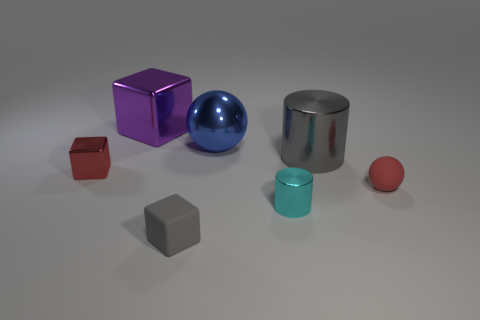
\includegraphics[width=.8\linewidth]{figures/CLEVR_example.png}
    \caption{Example of a generated image in the CLEVR dataset}
    \label{fig:clevr-example}
    % SD: Give also example of ground truth features that were used to generate this, i.e. objects and attributes.
    % DK: TODO
\end{figure}

Furthermore, the dataset contains information about each scene.
This includes all selected attributes for each object as well as the exact position of the centers of all the objects, both 3D-coordinates in the 3D scene and 2D-coordinates in the final rendered image.
In addition, simple spatial relations (in front of, behind, left, right) between the objects are calculated and stored.
% SD: For this, functions from the existing code are used, right?
% DK: exactly. Here, it is only described, what is part of the original CLEVR dataset (done)
These are simply based on the 3D-coordinates of the objects in relation to the position of the camera.

\subsection{Feature extractors}
\cmtDK[inline]{preprocessing}
In computer vision tasks, machines need to analyze images and extract information from them.
To do this, machines often rely on feature extractors.
Features are important parts or patterns in an image, which can have different levels of abstractions.
They can for example be low-level features, as geometric information about lines and edges in an image, or also very abstract information about whole objects.
Traditional approaches involve extracting key points and descriptors from an image and using them to represent the image \citep{Harris1988,Lowe1999,Bay2006}.
More recently, convolutional neural networks (CNN) became popular due to their ability to learn complex features automatically from raw image data.
These are also used in this thesis as a first layer to extract important information from the image. Hereby, two different architectures are tested.
\cmtDK[inline]{explain advantage of CNN}

First, we use the VGG19 \citep{Simonyan2015} which is an architecture based on many convolutional layers.
Using 16-19 convolutional layers with small convolution filters helps the model to solve localization and classification tasks on the training dataset, but also enables is to generalize onto other datasets.
After the convolutional layers, the data is passed first through an average pooling layer which outputs 512x7x7 dimensions.
Next follow three linear layers with \emph{ReLU} non-linearities in between.
After flattening the input, these classification layers output 4069, 4069 and 1000 dimensions respectively.

Secondly, we include the ResNet-101 \citep{He2016}.
This architecture tries to overcome the degradation of very deep networks, where the accuracy rapidly drops after it gets saturated.
This is done using residual blocks.
A residual block consists of two or three convolutional layers and a residual connection, also known as a shortcut connection.
The residual connection allows the input to be added directly to the output of the block, allowing the network to learn the residual function with respect to the input.
This approach enables the network to better preserve information from earlier layers and avoid the problem of information loss that can occur in very deep networks.
There are four blocks that output 256x56x56, 512x28x28, 1024x14x14 and 2048x1x1 dimensions.
A following average pooling layer outputs 2048x1x1 dimensions as well.
The final linear layer reduces the flattened data to 1000 dimensions, corresponding to the ImageNet classes.

Both architectures are available pretrained on an image classification task on the ImageNet dataset \citep{Deng2009}.
In this thesis, the implementations and weights available for PyTorch are used.\footnote{\href{https://pytorch.org/hub/pytorch\_vision\_resnet/}{https://pytorch.org/hub/pytorch\_vision\_resnet/}}\textsuperscript{,}\footnote{\href{https://pytorch.org/hub/pytorch\_vision\_vgg/}{https://pytorch.org/hub/pytorch\_vision\_vgg/}}
Since the task in this research is very different from a classification, it likely learned representations that are not directly transferrable to other tasks.
The pretrained knowledge in both models might not be directly transferrable to new tasks as studied by \citet{Yosinski2014}.
In this thesis, the task differs for multiple reasons.
First, the used images for the pretraining and the present study are part of a different domain.
Even though images of the CLEVR framework are generated to resemble the real world, they still only include abstract geometric objects while ImageNet contains real photos of persons, animals and objects.
Furthermore, the original task for the pretraining is a classification task, whilst this thesis is interested in generating and understanding referring expressions.
% SD: What are the differences? Mainly in the domain of objects and scenes. What data are VGG19 and ResNet trained on?
% DK: (added; done)
For this reason, multiple different adaptions of these architectures are compared.
Table \ref{tab:feature-extractor-archs} lists the different adaptions for both VGG19 and ResNet-101 that will be used in this research.
In the later chapters, it will be referred to these adaptions using the name in the table.

\begin{table}[ht]
    \centering
    \begin{tabular}{rlc}
        \toprule
                            & \textbf{description}                                            & \textbf{ output dimensions } \\\midrule
        \textbf{VGG-0}      & contains only the convolutional layers                          & 512 \times\ 7 \times\ 7      \\
        \textbf{VGG-avg}    & contains an additional average pooling layer                    & 512 \times\ 7 \times\ 7      \\
        \textbf{VGG-cls1}   & \makecell[cl]{contains an additional one classification layer,                                 \\ including its non-linearity} & 4069                         \\
        \textbf{VGG-cls2}   & \makecell[cl]{contains another additional classification layer,                                \\ including its non-linearity} & 4069                         \\
        \textbf{VGG-cls3}   & the original VGG19 architecture                                 & 1000                         \\\midrule
        \textbf{ResNet-1}   & contains one residual block                                     & 256 \times\ 56 \times\ 56    \\
        \textbf{ResNet-2}   & contains two residual blocks                                    & 512 \times\ 28 \times\ 28    \\
        \textbf{ResNet-3}   & contains three residual blocks                                  & 1024 \times\ 14 \times\ 14   \\
        \textbf{ResNet-4}   & contains four residual blocks                                   & 2048 \times\ 1 \times\ 1     \\
        \textbf{ResNet-avg} & contains an additional average pooling layer                    & 2048 \times\ 1 \times\ 1     \\
        \textbf{ResNet-cls} & the original ResNet-101 architecture                            & 1000                         \\
        \bottomrule
    \end{tabular}
    \caption{Different adaptions of VGG19 and ResNet-101 used in this research}
    \label{tab:feature-extractor-archs}
\end{table}

% Furthermore, we experimented with both the pretrained models as well as with the architectures trained from scratch with a random initialization for the weights.
% This reason for this was to test if the success of an experiment was actually making use of the pretrained knowledge incorporated in the models.
% SD: Link to the discussion on what datasets the systems are trained on.
% If that was not the case, the agents were likely not using image features, but instead relying on some other underlying patterns to solve the task.
% Basically, this approach works as an indicator to determine the actual success of the agents aside from measures as the accuracy or precision.
% SD: This is interestingly more complex and deserves much longer discussion. Pre-trained knowledge may be unhelpful if it is very different from the new domain. Hence, at some point training from scratch may be more successful. 
% SD: What is success? Learning may take longer but then after some time the performance is better than with pre-training. 
% SD: Since agents are free to invent new language it is not clear whether this will be align with the human language that influenced pre-training the visual models, hence there is both effect of domain and language here. 
% SD: We should make these questions part of a discussion, particularly if we are comparing the effects of pre-training vs training from scratch in the experiments.
% DK: learning from scratch not part of the thesis anymore, since not the focus and much more complex (done)

\subsection{Image processing}
\cmtDK[inline]{masking and how are they processed (convolutions to bring it to the same shape)}

The above described feature extractors are not enough to be solely used to encode the images used in this thesis.
Even though final layers that contain very task and domain specific knowledge can be removed, the previous layers still don't contain any information about the new domain and task.
For this reason they need to be extened with further layers that are not frozen and can learn and store information about the new domain by connecting the pretrained general knowledge with the specific task.
In this thesis, we use one architecture to encode images for all the conducted experiment.
The additional layers on top of the feature extractors however are always trained from scratch for each of the experiments and tasks.
By doing this, the models are made up of multiple smaller modules, as for example the image processing module or other modules that encode different inputs.
These modules can be added and combined step by step, whilst the architecture of each module always stays the same.
Following, the experiments stay comparable, since differences are only added or removed modules.

\citet{Johnson2017} describe an architecture that was used for training baseline models on the CLEVR dataset.
This architecture will be used for all experiments.
Hereby, the image is first passed through a frozen feature extractor.
Two convolutional networks with subsequent \emph{ReLU} non-linearities condense the important information from the output of the feature extractor.
The convolutional layers reduce the channels to 128 channels, using a kernel size of 3 and a stride and padding of 1.
Afterwards, a 2-dimensional max pooling is applied with a kernel size and stride of 2.
Finally, the resulting matrix is flattened and passed through a linear layer to reduce it to an encoding size.
This vector represents the encoded image with its extracted features.
Table \ref{tab:image_encoder} shows the layers and their output dimensions when using ResNet-3 as the feature extractor and an encoding size of 2048 dimensions.

\begin{table}[ht]
    \centering
    \begin{tabular}{cc}
        \toprule
        \textbf{layer}                      & \textbf{output dimensions} \\\midrule
        Input image                         & 3 \times\ 224 \times\ 224  \\
        ResNet-3                            & 1024 \times\ 14 \times\ 14 \\
        Conv(3 \times\ 3, \rightarrow\ 128) & 128 \times\ 14 \times\ 14  \\
        ReLU                                & 128 \times\ 14 \times\ 14  \\
        Conv(3 \times\ 3, \rightarrow\ 128) & 128 \times\ 14 \times\ 14  \\
        ReLU                                & 128 \times\ 14 \times\ 14  \\
        MaxPool(2 \times\ 2, stride 2)      & 128 \times\ 7 \times\ 7    \\
        Flatten                             & 6272                       \\
        Linear Layer(\rightarrow\ 2048)     & 2048                       \\
        \bottomrule
    \end{tabular}
    \caption{Image encoder with ResNet-3 and an encoding size of 2048}
    \label{tab:image_encoder}
\end{table}

\subsection{EGG framework}
The goal of this thesis is to run and compare different setups of language games systematically.
To do this, all experiments rely on the \emph{\textbf{E}mergence of lan\textbf{G}uage in \textbf{G}ames} (EGG) framework \citep{Kharitonov2019} which is implemented in PyTorch.
% SD: What is the framework? We saw that language games can be implemented very differently, with robots, as code, etc. it is a neural model.
% DK: (added; done)
This framework allows the implementation of language games in code, where agents are neural models that communicate with each other.
It consists of a heavily configurable core that controls the generating and parsing of the message, the calculation of the loss and the rules, for how the weights of all neural models are trained.
% SD: You frequently start discussion by referring to quite specific concepts straight away in a very concise way, e.g. Gumbel Softmax, Reinforce, without defining them but then an explanation comes later in the text. The problem with this a reader would wonder what they are and would look for explanation. It is best to have a very general introduction, e.g. we will test two optimisation functions and then introduce them and explain them in one go later.
% DK: (rephrased; done)
The configuration includes for example a choice between single symbol and sequence messages with varying RNNs, an easy switch between different loss functions or a choice between two optimization functions (Gumbel-Softmax relaxation and REINFORCE algorithms) to learn neural models containing discrete symbols.
% SD: More detailed description of all these. Readers will not be familiar with Gumbel-Softmax for example.
% DK: (rephrased; done)
Furthermore, runs of games can be saved to analyze the used messages of the agents and how they vary over the duration of the learning.

The EGG framework is set up in three levels.
Part of the lowest level are the \emph{agents} themselves.
The agents are neural models that need to be implemented from scratch and define how the agents process their input and in case of the receiver combine it with the message as well as what is their output.
The second level are \emph{wrappers} that take care of generating and parsing the message.
The sender wrapper uses the output of the sender agent, to produce a message.
The receiver on the other hand parses the message received by the sender and passes the result as an additional input to the receiver agent.
The third level, the \emph{game} links all described parts together.
It provides the agents with the input and passes the message from the sender to the receiver.
Furthermore, it uses the output of the receiver and calculates the loss, which is then the basis for the adaption of the weights for both wrappers and agents.
% SD: Include a diagram?
% DK: TODO

For the language games which are run in this thesis, the sender will always produce a sequence of symbols as a message, which the receiver will parse.
Gumbel-Softmax relaxation is applied to produce discrete symbols.
This is done in the default method of the EGG framework using two LSTMs, an encoder LSTM in the sender wrapper and a decoder LSTM in the receiver wrapper.
The output of the sender agent is used as the initial hidden state for the encoder LSTM.
% SD: This sounds like details of your implementation and should come later. Here, we would only need a general description of the EGG framework. Also for this text later, it would be good to have a diagram of all these steps and examples what these games actually are.
% DK: this is actually the default implementation in EGG in therefore described here (TODO, diagram)
This LSTM is then producing symbols until it generates an end-of-sequence symbol.
This sequence is then passed to the receiver wrapper with its decoder LSTM.
Its hidden state is initialized randomly.
The received message sequence is processed symbol by symbol.
After each time, a symbol is processed by the LSTM, the resulting new hidden state is passed to the receiver agent as the parsed message.
The receiver agent is combining it with its representation of the image input and is predicting an output.
In other words the receiver agent produces as many outputs as symbols are present in the message.
The \emph{game} is then calculating a loss for each of these outputs separately.
These losses are summed up to a total loss that is used to adapt the weights in both agents as well as in both LSTMs.

\subsection{Optimization in language games}
The traditional approach to solve problems with a discrete channel relies on the REINFORCE algorithm \citep{Williams1992}.
It uses the concept of Monte Carlo sampling to estimate the gradient of the expected cumulative reward with respect to the policy parameters.
The basic idea is to collect trajectories by following the policy, compute the cumulative rewards for each trajectory, and then update the policy parameters to increase the probabilities of actions that led to higher rewards.
% REINFORCE is easy to implement and understand, but it
REINFORCE suffers from high variance in gradient estimation due to the inherent randomness in the environment and the policy.
% SD: :-)
% DK: (done)

Gumbel-Softmax is a relaxation of the discrete categorical distribution to a continuous distribution that can be differentiated \citep{Jang2017}.
It allows for the application of gradient-based optimization methods to discrete optimization problems.
In the Gumbel-Softmax approach, randomness is introduced using the continuous Gumbel distribution.
Following, the \emph{softmax} operation creates a distribution over discrete actions that can be differentiated.
Gumbel-Softmax offers stable gradient estimates and can be more efficient than the traditional REINFORCE algorithm, especially when dealing with large action spaces.
This also applies to language games, where \citet{Havrylov2017} demonstrated that Gumbel-Softmax relaxation is more effective.
% SD: This is what a technical manual would say - but what does it do really? What is the difference between reinforce and Gumbel softmax in practice? In our case? Reinforce is still superior but here you make it less.
% DK: I don't think, REINFORCE is superior also in our case, since GS offers more stability in learning (see citing) (TODO, explain GS)

\subsection{Probing?}
\cmtDK[inline]{reason for usage and techniques fits more into theoretical background}

\subsection{Ethical considerations}
In the field of natural language processing (NLP) ethical issues often play major roles.
These can be part of the used datasets, the created models and their training as well as the application of the models.
For datasets, the role data privacy is increasing with the necessity of larger amounts of data \citep{Klymenko2022}.
Furthermore, datasets often contain biases, based for instance on the authors of the collected natural language texts. Often they also contain biases such as overrepresentations and underrepresentations.
Even though some of these biases are inherent to the data and not necessarily negative, much research is indicating that undetected and unaddressed biases in datasets might lead to negative consequences \citep{Shah2020,Field2021,Bender2021}.
Training neural models can also lead to environmental issues, as large models need to process huge amounts of data and require a lot of energy \citep{Bender2021}.
Finally, the application of trained models can create harm.
This applies for example to easy accessible large language model (LLMs) that can be used to create information hazard \citep{Weidinger2022}.

The research in this thesis tries to reduce these risks.
Looking at the datasets that are used in this thesis, all data is created artificially and contains therefore no personal information.
Even further, the aim of the creation of these datasets is to reduce and study the remaining biases.
% SD: to study biases
% DK: (rephrased; done)
It doesn't include any social information, but on the other hand consists only of abstract scenes.
The choice of which attributes the objects are made up is inherently biased towards human cognition, but doesn't have a social impact.
The models and agents are therefore trained, by including as few human biases as possible.

Looking at the environmental issues, the models used in this thesis consist of only few trained layers and the training is therefore short and doesn't require much energy.
Larger models as the feature extractors are already pretrained and add no additional consumption.

Finally, the purpose of this thesis is to analyze the results and the emerged language and draw conclusions, how emerged languages can be grounded better in the environment.
For that reason, the final models can't be uses in any real world applications and produce potential harm.
On the other hand, this work can on the long run mitigate harm as it provides a study of models, how they would behave on real data.
This therefore contributes towards interpretability of AI.
% SD: The work can on the long run mitigate harm as it is provides a study of models, how they would behave on real data and therefore contributes towards interpretability of AI.
% DK: (added; done)

\newpage

\section{Creation of the datasets}
\label{sec:creation-dataset}
This research investigates how agents use referring expressions to discriminate objects seen in images based on their relations.
For that reason, the original CLEVR framework offers too little control over how a new dataset is created.
Especially, which objects and in which attributes they share with each other in each image can't be controlled.
Following, we extended the framework for generating new datasets.\footnote{\href{https://github.com/DominikKuenkele/MLT\_Master-Thesis\_clevr-dataset-gen}{https://github.com/DominikKuenkele/MLT\_Master-Thesis\_clevr-dataset-gen}}
By this, the objects in the generated images are controlled to have different human-recognizable attributes, namely the \emph{shape}, \emph{size} and \emph{color}.
These attributes also correspond to referring expressions in natural language such as English.
% To simplify the generation and the succeeding training of the models, we only focused on the attributes with a high impact on the appearance of the object, namely the \emph{shape}, \emph{size} and \emph{color}.
The \emph{material} is always the same for all objects in a generated image.
There were three main extensions to the framework:
% SD: Too informal
% SD: We create a new dataset based on the CLEVR framework where we control the appearance of scenes in a referring expression task.
% SD: The scenes are controlled by human-recognisable attributes of object such as object shape, colour and type. These attributes also correspond to referring expressions in natural language such as English.
% SD: We create two contexts of scenes, one with two objects and one with five. 
% SD: We also control for the number of attributes shared between the target and the distractor.
% DK: creation of dataset later (here only the general rules), (added; done)

First, objects in the scene were separated into three categories: one \emph{target object}, objects in a \emph{target group} and \emph{distractor} objects.
The target object is the main object in the scene and the models are trained to identify and communicate between each other.
All other objects and their relations are based on this target object.
The target group contains similar objects to the target object.
These are objects that the agents need to discriminate the target object from.
Finally, the distractors are objects that add noise to the scene and should make it more complex. They are expected to teach the agents more precise descriptions of the target object.
The number of the objects in both groups can be controlled.

In a second step, when generating the images it is possible to define the relations between \emph{target object}/\emph{target group} and \emph{target object}/\emph{distractors}.
The relation is defined as \textbf{how many} attributes of the target object are identical with the attributes of a single object in the target group and distractors respectively.
For example the target object is a \emph{small red cube}.
If two attributes are shared between target object and target group, objects in the target group could include \emph{small blue cube}, \emph{big red cube} or \emph{small red sphere}, but couldn't include another \emph{small red cube} or a \emph{small blue cylinder}.
The number of shared attributes can also be set to a range to control how challenging the referring task is.
% SD: To control how challenging the referring task is
% DK: (done)

Lastly, it is also possible to define exactly \textbf{which} attributes should be shared between the target object and the groups.
For example, it can be defined to have the same size for objects in the target group, but have different, randomly selected shapes and colors.
This allows for a very controlled generation of relations between the objects in the scene.
% SD: Introduce other images earlier?
% DK: I think 'Dale-5' is the most interesting image to make the point here. The others are introduced later, in the order of the pictures. So I don't think I also can change the order the pictures. (done)
Figure \ref{fig:clevr-dale-5} shows one generated image with this extended source code.
Here, the target object is the large purple cylinder.
The target group contains four objects that share zero to a maximum of two attributes.
It is not controlled, which attributes are shared (they are selected randomly). The large purple cylinder shares the same color and size with the large purple sphere, the same size with both cubes and no attribute with the small turquoise sphere.
There are no distractor objects.
% SD: It depends what you mean by distractor objects. I’d say they are all distractor objects by the virtue they share attributes. The system has to learn understanding of an intersection of these attributes.
% DK: I refer to the definitions in the paragraphs above, namley target object, target groub and distrctors. (done)

For all generated datasets in the following sections, the general constraints and settings are as close as possible to the original CLEVR dataset.
The size of the generated images is 480x320 pixels.
10.000 images are created for each of the datasets.
Each image contains a maximum of 10 objects, that are not intersecting, have the same minimum distance between objects and are at least partially visible from the camera.
% SD: Note that since objects are generated as a part of 3-d scenes, they may appear differently on images: size, occlusion, shading, rotation. We also expect the model to learn from this noise and which therefore makes the task much harder and a task that approximates natural environment compared to the task where we would use abstract geometric shapes projected on a 2-d plane.
% DK: added in the general description of CLEVR since it is not my extention (done)
% TODO: we create the follwoing dataset ....

\begin{figure}[ht]
    \centering
    \subfigure['CLEVR single', \emph{large yellow sphere}]{
        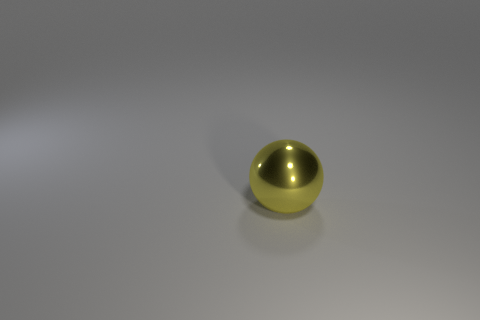
\includegraphics[width=0.43\linewidth]{figures/CLEVR_single.png}
        \label{fig:clevr-single}
    }
    \subfigure['CLEVR color', \emph{small brown cylinder}]{
        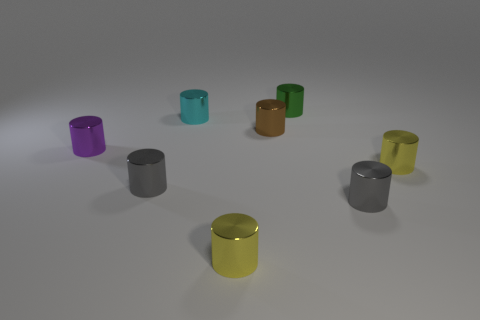
\includegraphics[width=0.43\linewidth]{figures/CLEVR_color.png}
        \label{fig:clevr-color}
    }
    \subfigure['Dale-2', \emph{small green cylinder}]{
        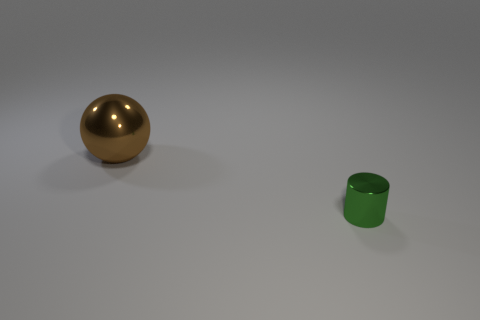
\includegraphics[width=0.43\linewidth]{figures/CLEVR_dale-2.png}
        \label{fig:clevr-dale-2}
    }
    \subfigure['Dale-5', \emph{large purple cylinder}]{
        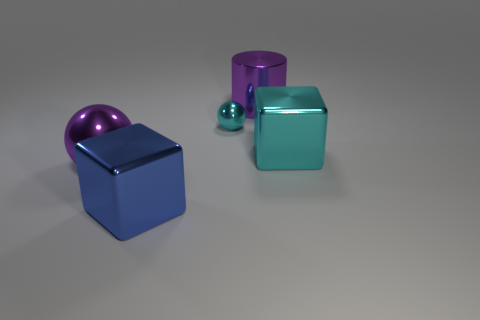
\includegraphics[width=0.43\linewidth]{figures/CLEVR_dale-5.png}
        \label{fig:clevr-dale-5}
    }
    \caption{Example images of each dataset, with the target object specified}
    \label{fig:clevr-examples}
\end{figure}

\subsection{CLEVR single}
The simplest new dataset is called 'CLEVR single'.
This is a very simple dataset and has the purpose to simplify the problem the model needs to learn as much as possible.
Each scene in the dataset contains only one single object, the target object.
There are neither objects in the target nor in the distractor group.
All attributes are assigned randomly to the target object.
The differences across the whole dataset are the locations and rotations of the objects.
With this dataset, neural models can focus on only the features, as well as the locations of this single object.
There are no objects that distract the model from extracting features from the target object.
This helps to understand if the models are actually able to assign features or learn locations of these features in an image.
Figure \ref{fig:clevr-single} shows an example with the only object being the \emph{large yellow sphere}.

\subsection{CLEVR color}
The second dataset that is created is called 'CLEVR color'.
The purpose of this dataset is to create scenes, where the target object is completely unique and as easily identifiable as possible.
For this reason, there exist only two groups in the scene, the target object and distractors.
The distractor group can contain in between 6 and 9 objects.
To make the discrimination as simple as possible the target object and the objects in the target group share exactly two attributes.
% SD: Wouldn’t it make sense to introduce the discussion of how scenes can be generated with attributes somewhere here? Again, I felt we were projecting forward earlier without understanding the task.
% DK: before, I only wanted to outlie the rules for the creation, i.e. what is possible with it. Since the code to create the datasets is also a contribution, I wanted to let it stand on its own. Here I only describe how these rules are applied for each new dataset. (QUESTION)
Furthermore, to simplify the relation between target object and distractors over the whole dataset, it is also controlled which attributes are shared.
The distractors have always the same size and shape as the target object, but the color is different.
The reason for choosing the color as the only discriminating attribute is that it is assumed that the color is easier to learn for neural models as opposed to for instance abstract shapes.
% SD: But why not test the limits and the harder examples?
% DK: In the experiments, the models often hda problems to learn anything (with the complex dataset), which is why I reduced the complexity with the 'color' dataset. (done)


As seen in Figure \ref{fig:clevr-color}, the \emph{small brown cylinder} is unique.
By this, it is possible to refer to the target object using the attributes with four different combinations: the \emph{brown} object, the \emph{brown cylinder}, the \emph{small brown} object and the \emph{small brown cylinder}.
All attributes, apart from the color are not discriminating the target object from the distractors.
Notice as well that this restriction doesn't apply to the distractors, where multiple objects with the same color are allowed.
In other words, the choice of attributes is random for the distractors, and they may overlap.
% SD: In order words, the choice of attributes is random for distractor and there may be an overlap between the same distractor objects. This is because we do not control overlap attributes over distractor, I.e. random.
% DK: (added; done)

\subsection{CLEVR Dale datasets}
% SD: In the previous dataset the target and distractor are discriminated by ONE attribute exactly.
% DK: TODO
The above described dataset is very restrictive in the relation between the objects, where only \emph{one} attribute is used to disambiguate them.
The number and the type of shared attributes are controlled exactly.
In the real world, objects have overlapping attributes and hence objects can only be identified by an intersection of multiple attributes.
In real situations, there is no restriction at all how objects or things relate to each other.
Natural language emerged that can refer to distinct attributes of these objects to discriminate them from each other.
This emergence of referring attributes and their combination is studied deeper in this work.
% SD: In real world, objects have over-lapping attributes and hence a single object can only be identified by an intersection of attributes.
% DK: (rephrased; done)

% SD: However, we do not do this randomly but ge5 inspiration from the Dale and Reiter generation algorithm who observe that attributes in descriptions occur in certain order and are added incrementally in a certain hierarchy. This way we approximate the information in the scenes to human cognition and we hope that the system will be able to exploit that (we would really need to study and compare it with another dataset where attributes are add3d randomly to confirm that there is an effect of h7man. Ignition).
% DK: see below (done)
For this, we created a dataset that allows almost any relation between a target object and the distractors.
However, the creation is inspired by incremental algorithm for the Generation of Referring Expressions (GRE) described in \citep{Dale1995} who observe that attributes in descriptions occur in certain order and are added incrementally in a certain hierarchy.
This algorithm ensures that every scene contains a unique object in respect to its and the distractors' attributes.
Using the algorithm, one can refer to an object using its attributes to discriminate it from all other objects as efficiently as possible.
In other words, the object is described unambiguously using the lowest number of words.
For the dataset that means that zero, one or two attributes can be shared between the target object and distractor objects.
This ensures the uniqueness of the target object.
On the other side, it is not controlled which attributes are shared.
% SD: The sharing of attributes should be according to the Dale and Reiter hierarchy, shouldn’t it? Two attributes, big blue (cube|sphere)
% DK: During the creation of the dataset, only the number of shared attributes is shared that we get different numbers of overlaps. Only the captions (that are created later and used as input or output for some models/agents) rely directly on the algorithm. At this point, I only wanted to bring up the reason for this, which is the usage of the algorithm in human referring expressions and how it compares to machine referring expressions. (done)
These are assigned randomly.
There is again no control over the relations between distractors, which means that distractors can appear multiple times.

Two datasets following these rules are created.
The Dale-2 dataset contains one target object and one distractor (see Figure \ref{fig:clevr-dale-2}), while the Dale-5 dataset contains one target object and exactly four distractors.
Consider Figure \ref{fig:clevr-dale-5}, with the target object being the \emph{large purple cylinder}. The large purple sphere shares the size and color, the two cubes only share the size, and the small turquoise sphere doesn't share any attribute.
% SD: It’s actually the reverse in which descriptions are generated, we start left to right: large purple (are shared), the last attribute must thus be unique. Generation proceeds in the opposite order, one would just say sphere. We should clarify this. Now it is very hard to understand.
% DK: That's true for the generation of the descriptions. This is explained in chapter 4.2.1 where the captions are needed for the training as input. As said before, the algorithm was not directly used and is just the reason. (done)

These two datasets allow a more realistic look in how models can acquire knowledge about attributes of objects.
More specifically it helps to understand how models learn to discriminate objects from each other, since the model may only need to learn discriminative features of objects and not all features of the whole object.

\cmtDK{probabilities of shared attributes for both Dale-2 and Dale-5}
\newpage

\section{Grounding referring expressions}
\label{sec:preexperiments}

This chapter serves two purposes.
First, the generated dataset from the precious section is validated.
For this, models are trained to both generate referring expressions of the target object and understand existing referring expressions.
A success of these experiments indicates that the target objects in the datasets are possible to refer to and the datasets can be used in more complex setups in language games.

Secondly, the experiments in this chapter provide the basis for the setup of the agents in the language games.
Language games are very complex setups for machine learning models.
The models need to solve multiple tasks at the same time in order to solve the overall problem.
For instance, in a simple setup of a game two agents are involved.
The first agent, the sender, is shown a scene with objects and needs to communicate one target object to the other agent, the receiver.
The receiver is shown the same scene and needs to identify the target object with respect to the message of the sender.
In this case, the sender first needs to learn to encode the scene, all objects and their attributes, as well as the information about the target object into its own game specific space.
In a next step it needs to learn how to translate this encoding into a message that is sent to the receiver.
The receiver then needs to learn to decode this message, after which it needs to learn how to combine the decoded message with its own encoding of the scene and objects.
And finally it needs to learn how to identify the target object with this information.
There are many points of possible failure to train the agents.
% SD: This should go at the beginning where language games with neural agents are introduced.
% DK: TODO

For this reason, we decided to divide the main problem and let the models learn simpler subtasks and increase the complexity step by step.\footnote{\href{https://github.com/DominikKuenkele/MLT\_Master-Thesis}{https://github.com/DominikKuenkele/MLT\_Master-Thesis}}
This will give a very detailed overview where the models struggle to learn and in which ways they can be improved.
Mainly, the tasks are separated into language games with two agents and classical machine learning tasks without any communication, namely only one 'agent' that solves the task alone.
With this division, we can analyze the learning of the encodings of the scenes separately from the learning of producing and decoding messages.

% TODO maybe move to front...
The final objective of this thesis is to find out, how agents can communicate about relations of objects based on their attributes, namely how to generate and understand referring expressions.
Because of that, the first experiments focus on extracting information from images and combining them with structured knowledge about the objects.
Here, we structured the experiments into three levels.
In the first level, the models are trained to learn the position of objects in the image and attend to specific regions of the image, by understanding a referring expression of the target object.
% SD: This is a natural language understanding or reference resolution task.
% DK: TODO maybe put into methods...
In the second level, the models are trained to differentiate objects in the scene from each other, again by understanding referring expressions.
% SD: Object identification task
% DK: TODO
In the last level, the models are trained to generate referring expressions, more specifically the models learn to caption and describe objects in the image.
% SD: Referring expression generation task
% DK: TODO
These combined experiments should lay the basis for how to build up the agents in the language games.
% SD: We are validating the dataset on 3 tasks
% DK: TODO

\subsection{Object identification}
\label{sec:object-identification}
\subsubsection*{Setup}

In a first task a neural model is trained to discriminate multiple objects from each other.
Hereby, the model is shown bounding boxes of all objects in the scene as well as a description of the target object.
The model needs to combine all information and then point to the correct bounding box.
This task forces the model to extract visual features from the objects in the shown inputs and connect them to a representation of human given attributes.
Since the model is shown only bounding boxes around each object rather than the whole scene, geometric information about the objects' locations doesn't play a role for the success in this task.

In a first step, bounding boxes are extracted from each scene.
Each bounding box is a square with a side length of 96 pixels around the center coordinates of each object.
By doing this large objects in the front of the scene fill the bounding box completely, while smaller objects in the back of the scene contain some space around them.
They also might contain noise in the form of parts of adjacent objects.
Preliminary experiments indicated however that a more complex method for extracting the bounding boxes, depending on spatial position in the scene to reduce the noise didn't improve the results.
Therefore, bounding boxes in this thesis rely on the former simpler approach.
Since, each bounding box will be passed through on of the feature extractors, described in section \ref{sec:feature-extractors} they need to be normalized first.
As described in \citep{He2016,Simonyan2015}, the bounding boxes are resized to 256 pixels for the shorter side, then cropped around the center to a square of 224 \times\ 224 pixels.
Finally, the RGB channels are normalized, by subtracting the means (0,485; 0,456; 0,406) and dividing the result by the standard deviation (0,229; 0,224; 0,225) for each channel respectively.
The array of bounding boxes is padded with matrix of zeros to the maximum possible number of objects present in a scene across the dataset.
For the 'Dale-2' dataset, this corresponds to a maximum of two bounding boxes, 5 bounding boxes for the 'Dale-5' dataset and 10 for the 'CLEVR color' dataset.
For each sample in the dataset the bounding boxes are shuffled.

The attributes of the target object are encoded as one-hot encodings.
There is a three-dimensional vector encoding the \emph{shape}, an eight-dimensional vector encoding the \emph{color} and a two-dimensional vector encoding the two different \emph{sizes}.
The values of each dimension of these vectors can either be zero or one, depending on the attributes of the target object.
These three encodings of the attributes are then concatenated to a vector with 13 dimensions.

\begin{figure}[ht]
    \centering
    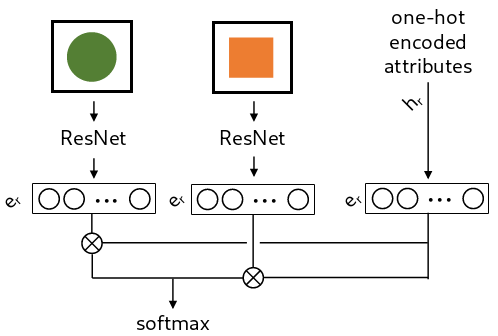
\includegraphics[width=.5\linewidth]{figures/arch_bounding_box_classifier.png}
    \caption{Simplified architecture of the object identification task}
    \label{fig:bounding_box_classifier_architecture}
    % SD: I haven't commented on this before, but let us be very careful in naming all meta-paramaters of the models in the text or in caption: how many layers, how many dimensions, etc. The reader should be able to replicate the code and the experiment from this. You can do this in the caption which is a longer explanation or in the text itself.
    % DK: TODO
\end{figure}

The model, the \emph{object identifier} is split into two parts.
First, each normalized bounding box of the sample is passed through \emph{ResNet-avg}.
The preceding layers \emph{ResNet-1} to \emph{ResNet-4} couldn't be compared due to memory restrictions on the GPU.
A deeper analysis of the effects of different feature extractors will be done in the following chapters.
The resulting vector is flattened and projected to the embedding dimension $e$ via a linear layer.
% SD: This is quite low? Why only 10?
% DK: different embedding sizes are tested (done)
Correspondingly, the one-hot vector of the attributes is projected to the same embedding dimension with another linear layer.
In the second part, each bounding box is combined with the representation of the attributes.
By bringing both vectors to the same embedding size, the dot product between each embedded bounding box and the embedded attributes can be calculated.
A high correlation between the attributes and the object should result in a high dot product, while a low correlation results in a lower dot product.
The model can so learn to connect the object representation with the attributes.
The dot products are concatenated and form a vector with as many dimensions as objects present.
The \emph{softmax} function is applied over the resulting vector, which returns a probability distribution over all objects; the model points to the object with the highest probability.
% The model then points to an object, using the \emph{softmax} function over this resulting vector.

The experiments are conducted with the following hyperparameters: a learning rate of $2\times10^{-4}$, a batch size of 32 samples and 30 epochs, \emph{Adam} \citep{Kingma2015} as optimizer.
The number of epochs was chosen manually after identifying when the loss as well as the test accuracies didn't improve significantly.
8000 randomly selected samples are used for training, the remaining 2000 samples for testing.
The loss is calculated using cross entropy.
The following embedding dimension $e$ are compared: 2, 10, 50, 100, 500, 1000.
% SD: So, the output of this model is a vector of 0 and 1s, with the 1 identifying the corrct object (or the other way around?).
% DK: the output is a probability distriution over all objects (inserted above; done)

The object identification task is trained on all datasets that include more than one object in each sample, namely the 'CLEVR color', 'Dale-2' and 'Dale-5' dataset.
Random baselines for each dataset would yield accuracies of 10\%, 50\% and 20\% respectively.
% excluding the 'CLEVR single'.
% SD: Why not?
% DK: because there is only one object in the input, and therefore only one possible guess. The model can't point to a distractor (adressed; done)
The 'Dale' datasets are directly comparable to each other for the similar setup of their creation.
Especially interesting is the effect of the increasing the number of distractors and the growing number of attributes that are needed to discriminate the objects.

\subsubsection*{Results}
As expected, all baselines achieve a random accuracy for each of the datasets.
The accuracy lies at 50\% for the 'Dale-2' dataset, 22\% for the 'Dale-5' dataset and 12\% for the 'CLEVR color' dataset.
This changes however, when information about the target object is included.
Table \ref{tab:results_bounding_box_classifier} lists the accuracies of the models' predictions after 10 epochs.

\begin{table}[ht]
    \centering
    \begin{tabular}{c|c|c|c}
        \toprule
               & \textbf{Dale-2}   & \textbf{Dale-5}   & \textbf{CLEVR Color} \\\cmidrule(lr){2-2}\cmidrule(lr){3-3}\cmidrule(lr){4-4}
        $e$    & \textbf{Accuracy} & \textbf{Accuracy} & \textbf{Accuracy}    \\\midrule
        {2}    & {92\%}            & {72\%}            & {40\%}               \\
        {10}   & \textbf{100\%}    & {94\%}            & {92\%}               \\
        {50}   & {99\%}            & \textbf{95\%}     & \textbf{94\%}        \\
        {100}  & \textbf{100\%}    & \textbf{95\%}     & {93\%}               \\
        {500}  & \textbf{100\%}    & \textbf{95\%}     & {93\%}               \\
        {1000} & \textbf{100\%}    & {94\%}            & \textbf{94\%}        \\
        \bottomrule
    \end{tabular}
    \caption{Accuracy scores of the object identifier: $e$ are different embedding sizes}
    \label{tab:results_bounding_box_classifier}
\end{table}

\begin{table}[ht]
    \centering
    \begin{tabular}{cc|ccc|ccc|ccc}
        \toprule
                                        &                           & \multicolumn{3}{c}{\textbf{dale-5}} & \multicolumn{3}{c}{\textbf{dale-2}} & \multicolumn{3}{c}{\textbf{colour}}                                                                                                                                                             \\  \cmidrule(lr){3-5}\cmidrule(lr){6-8}\cmidrule(lr){9-11}
        coordinate-classifier-dimension & image-embedding-dimension & \textbf{accuracy}                   & \textbf{word-by-word-f1}            & \textbf{non-target-accuracy}        & \textbf{accuracy} & \textbf{word-by-word-f1} & \textbf{non-target-accuracy} & \textbf{accuracy} & \textbf{word-by-word-f1} & \textbf{non-target-accuracy} \\\midrule
        {10}                            & {1500}                    & {33\%}                              & {67,47\%}                           & {14\%}                              & {84\%}            & {81,42\%}                & {4\%}                        & {12\%}            & {33,43\%}                & {34\%}                       \\
        {10}                            & {2000}                    & {36\%}                              & {69\%}                              & {13\%}                              & {83\%}            & {82,89\%}                & {4\%}                        & {13\%}            & {36\%}                   & {34\%}                       \\
        {10}                            & {3000}                    & {34\%}                              & {68\%}                              & {12\%}                              & {82\%}            & {79,89\%}                & {4\%}                        & {12\%}            & {32,31\%}                & {34\%}                       \\
        {15}                            & {1500}                    & {35\%}                              & {68,99\%}                           & {12\%}                              & {85\%}            & {84,43\%}                & {4\%}                        & {17\%}            & {38,49\%}                & {31\%}                       \\
        {15}                            & {2000}                    & {34\%}                              & {67\%}                              & {14\%}                              & {84\%}            & {81,89\%}                & {4\%}                        & {14\%}            & {33,31\%}                & {33\%}                       \\
        {15}                            & {3000}                    & {32\%}                              & {65,5\%}                            & {15\%}                              & {85\%}            & {81,89\%}                & {4\%}                        & {13\%}            & {32,73\%}                & {35\%}                       \\
        {30}                            & {1500}                    & {36\%}                              & {68,99\%}                           & {15\%}                              & {84\%}            & {80,95\%}                & {4\%}                        & {14\%}            & {36,97\%}                & {33\%}                       \\
        {30}                            & {2000}                    & {32\%}                              & {65,5\%}                            & {16\%}                              & {85\%}            & {82,95\%}                & {4\%}                        & {18\%}            & {39\%}                   & {32\%}                       \\
        {30}                            & {3000}                    & {3\%}                               & {63,5\%}                            & {16\%}                              & {83\%}            & {80,89\%}                & {3\%}                        & {12\%}            & {32,73\%}                & {34\%}                       \\
        {100}                           & {10}                      & {21\%}                              & {57\%}                              & {23\%}                              & {16\%}            & {37\%}                   & {31\%}                                                                                                     \\
        {100}                           & {15}                      & {17\%}                              & {52,98\%}                           & {25\%}                              & {78\%}            & {71,99\%}                & {11\%}                       & {26\%}            & {43,49\%}                & {3\%}                        \\
        {100}                           & {30}                      & {19\%}                              & {54,46\%}                           & {24\%}                              & {68\%}            & {42,79\%}                & {4\%}                        & {29\%}            & {45,49\%}                & {26\%}                       \\
        {500}                           & {10}                      & {27\%}                              & {61,98\%}                           & {16\%}                              & {83\%}            & {79,95\%}                & {6\%}                        & {17\%}            & {38,49\%}                & {32\%}                       \\
        {500}                           & {15}                      & {28\%}                              & {63,5\%}                            & {16\%}                              & {83\%}            & {79,5\%}                 & {7\%}                        & {21\%}            & {4\%}                    & {31\%}                       \\
        {500}                           & {30}                      & {3\%}                               & {63,98\%}                           & {17\%}                              & {84\%}            & {83,43\%}                & {5\%}                        & {21\%}            & {4\%}                    & {31\%}                       \\
        {1000}                          & {10}                      & {31\%}                              & {65,5\%}                            & {13\%}                              & {84\%}            & {82,42\%}                & {5\%}                        & {12\%}            & {32,12\%}                & {34\%}                       \\
        {1000}                          & {15}                      & {31\%}                              & {64,5\%}                            & {16\%}                              & {85\%}            & {82,42\%}                & {5\%}                        & {16\%}            & {37\%}                   & {32\%}                       \\
        {1000}                          & {30}                      & {31\%}                              & {63,98\%}                           & {17\%}                              & {85\%}            & {82,81\%}                & {4\%}                        & {13\%}            & {36\%}                   & {34\%}                       \\
        \bottomrule
    \end{tabular}
    \caption{test}
    \label{test}
\end{table}
The model achieves almost perfect accuracy on the 'Dale-2' dataset with 99\%.
For both other datasets, the accuracy is slightly lower with 94\% and 93\% respectively, but still close to perfect, especially compared to the random baseline.
First, this shows that the model is able to extract attribute features from the image and manages to combine them with the given information about the target object.
This worsens slightly, when more objects are introduced.
More objects lead to more needed attributes to discriminate the objects from each other.
The model is still able to extract and utilize these additional attributes and combine them with the given attribute encoding of the target object.
The model can generate these high results, even with its relatively simple architecture.
In this architecture, the model doesn't compare the objects directly to each other, but each object is only associated with the attribute encodings.
A more complex architecture, in which the model is additionally tasked to discriminate the objects directly from each other might even improve the results.
% SD: The model is able to leatn to discriminate objects based on visual appearance.
% DK: TODO

\subsection{Referring expression generation}
\label{sec:referring_expression_generation}
\subsubsection*{Setup}
\cmtDK[inline]{new metrics}

Opposed to the previous experiment, where the focus lied on extracting visual features, the model is now tasked to generate referring expressions.
This is done in two setups.
The first setup uses bounding boxes as in the previous section as input, where the model needs to describe the target object of one of the bounding boxes.
In the second setup, the model is presented with the complete image and therefore also needs to accommodate to geometric information of the scene.

The bounding boxes are extracted and normalized in the same way as for the object identification task.
Since for the second setup, the images will also be passed through the feature extractors, they are normalized as well in like manner.
The referring expressions for the target object are generated using the incremental GRE-algorithm, described in section \ref{GRE}.
By this, the model needs to describe the target object with respect to the distractor objects.
There are some minor additions concerning the padding of the referring expression.
As before, the referring expression is padded to a number of three tokens, corresponding to the maximum of three attributes.
However, there are three different ways how the padding is applied.
First, the referring expression are, as usual in captioning tasks padded at the end with a specified padding token.
A problem could arise when the referring expression is not viewed as a natural language sentence, but as slots filled with tokens.
More specifically, following the GRE-algorithm, the last token in the referring expression is always the shape.
The second last token if existing describes the color, while the third last token if existing describes the size.
As soon as this sequence is padded at the end, these slots disappear.
A referring expression that only describes the shape, such as \emph{cube} will be padded to \emph{cube <pad> <pad>}, where the third last slot is filled up with the shape instead of the size.
Since this task is not focussing on producing natural language with a correct grammar, but focuses instead on extracting attributes, having a slot structure could help the model to express the extracted attributes correctly.
For this reason, the second method of padding the referring expression is prepending the referring expression with padding tokens.
By this, the positions of the slots are preserved and if not specified just filled with a padding token.
Each slot has always the same semantic value, e.g. the last slot always contains the shape of an object.
This can be done since the referring expressions are not free text, but instead the structure and the possible content is given by the dataset.
This method might help the model to learn the correct referring expressions.
% SD: Slots have the same semantic value, i.e. the last slot is the object type. We can do this because we know the structure of the descriptions in this dataset and because we hope this will help the learning. Also, we are thinking of generation based on slots.
% DK: (addressed; done)
The last variation concerns the order of producing each token.
When the referring expressions are prepended, the model would need first produce two padding tokens, before it finally can produce a much more meaningful token for the shape.
This could be difficult to learn for a model, as the longer a sequence of tokens is, the more information about the beginning of the sequence gets lost.
Even though a sequence of just three tokens may not be long enough for this factor to be a problem, we experimented to reverse the referring expression.
% SD: We... I sounds more like you are writing a lab report with casual language but here you want to be more formal.
% DK: (done)
Instead of producing for instance \emph{<pad> green sphere} as correct in English, the model would now need to produce \emph{sphere green <pad>}.
Notice that the padding token is again at the end of the generation, but the order of slots as well as the amount of information in the referring expression are still preserved.

This task inherently involves learning human knowledge and natural language structure.
Nonetheless, this helps to understand more detailed if and how the model discriminates objects.
Can the model solve the task, or do specific attributes used by humans pose challenges to the model?
% Does it rely on the same attributes humans are using, or does it find other important differences, or is it not able to solve the task at all?
% SD: In this case it should be using the same attributes as humans as we are training it on human labels.
% DK: (rephrased; done)

% TODO include figure

In the first setup, the \emph{bounding box RE generator}, the model receives the bounding boxes as input.
The first bounding box is always the target object, while the remaining bounding boxes are shuffled.
As in the previous experiment, each bounding box is passed through \emph{ResNet-avg} and projected afterwards to an image embedding dimension $e$ with a linear layer.
All thus encoded bounding boxes are concatenated and again compressed to the decoder output dimension $LSTM_o$ using another linear layer.
This representation of all objects serves as the initial hidden state of an LSTM, which generates the referring expression.
Tokens used in the LSTM are embedded with embedding dimension $LSTM_e$.
During training, teacher forcing is applied by using embeddings of the ground truth tokens as the input sequence for the LSTM, instead of the output of the LSTM.
The output of the LSTM is passed through a linear layer at each step to determine logits over the symbols of the vocabulary.
During testing, the LSTM is always forced to generate three tokens, with an embedded start-of-sequence token as first input to the LSTM.
Each token in the sequence is determined greedily, by selecting the highest logit in the output of each step in the LSTM.

\begin{figure}[ht]
    \centering
    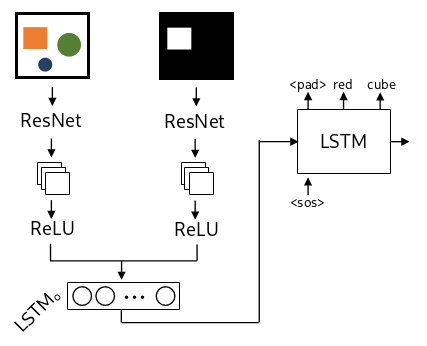
\includegraphics[width=.5\linewidth]{figures/arch_caption_generator.png}
    \caption{Simplified architecture of the masked caption generator}
    \label{fig:caption_generator_architecture}
\end{figure}

In the second setup two different models are compared against each other.
The first model, the \emph{basic RE generator} acts as the baseline and only receives the complete image as the input.
The image is passed through \emph{ResNet-3} and subsequently processed by additional convolution layers, described in section \ref{sec:image-processing}.
The resulting vector is then reduced to decoder output dimension $LSTM_o$ by a linear layer and as for the bounding boxes acts as the initial hidden state for the LSTM.
The LSTM is trained in the same way as above.

Using this approach, the model doesn't have any information about the target object and is therefore expected to produce referring expressions for a randomly selected object on the scene.
Therefore, it is extended in a second step with attention to the target object, the \emph{masked RE generator}.
% SD: You add attention to the target object.
% DK: (added; done)
A masked version of the image is created and passed to the model.
For this, a fixed size squared area of 96 \times\ 96 pixels around the center of the target object is filled in white, while the rest of the image is filled in black.
Both original and masked image are processed together with convolutional layers as described in section \ref{sec:image-processing}.
% SD: This is normally implemented as a filter of 1 and 0 corresponding to pixels. As such it then corresponds to attention, cf. paper with Mehdi.
% DK: (QUESTION)
The result is then again projected to the decoder output dimension $d$ by a linear layer and then used as the initial hidden state for the LSTM.
This should point the model towards which object to describe and discriminate from the distractors.

For both setups, the same hyperparameters as in the previous experiments are used: a learning rate of $2\times10^{-4}$, a batch size of 32 samples and 30 epochs, \emph{Adam} \citep{Kingma2015} as optimizer.
8000 randomly selected samples are used for training, the remaining 2000 samples for testing.
The loss is calculated using cross entropy.
The following values for the variables are compared:
\begin{itemize}
    \item $e$ (only for bounding boxes): 100, 500, 1000
    \item $LSMT_o$: 100, 500, 1000
    \item $LSTM_e$: 10, 15, 30
\end{itemize}

As already discussed before, this task can be interpreted as a classification task rather than a natural language generation task.
The main reason for this is that the model is tasked to assign specific attributes to the target object instead of producing free text with a large vocabulary.
Following, we are interested in the classification mistakes the model makes.
For this, the model's success is validated on accuracy, recall and precision scores.
These are calculated in the following ways.
The first measure is the \textbf{overall accuracy} if the model predicted every word in the caption correctly.
% SD: This is too strict. if this is a generation task then we can use generation metrics. Those compare if the generated string as a whole is kind of similar to the target string, see ROUGE, METEOR, BERTscore.
% If this is a classification task, and it is, given that we know what type of word we expect in each slot, we could calculate accuracy per class, precision, recall, F-score. We could also calculate mean ranks for predicting words per classes, or acucracy at k- if the target word is in the k-top predictions.
% We could also take it a multi-class classification problem and how to calculate accuracy in this case, would need to check.
% DK: I agree that classification metrics refelct success better here (therefore I also used accuracy). These metrics would give a better overview, but I don't think there is time to implement it (QUESTION)
This gives a hint, how the model fares in general and if it is able to predict any of the attributes.
However, a 'false' prediction doesn't give much insight into why the model predicted a wrong caption.

It could be the case that the model predicted the correct shape, but wrong color.
Even worse, the model could have predicted more attributes than necessary to uniquely identify the target object and didn't follow the rules of the GRE-algorithm.
For instance, consider the scene in Figure \ref{fig:clevr-dale-5}.
% SD: Too far away, might be worth repeating here, you say still stay Fiigure 2d, repeated asFigure 6 here
% DK: TODO
The correct caption is \emph{cylinder}.
If the model would predict \emph{purple cylinder}, the accuracy determines it as false as captioning \emph{large purple cylinder} as well \emph{small green cube}.
The first two descriptions identify the target object perfectly, but the model only didn't learn to exclude unnecessary attributes.
To mitigate this, the accuracies for each class are included, as well as the macro average.
% SD: Is this figure for a particular class, i.e. object type, or do you then do something to individual accuracy, i.e. average them?
% DK: the metric is averaged over all samples (not by class). Might be definitly worth to do it class by class. Time? (QUESTION)
This can give a better understanding of the errors the model makes.
The same is done for \textbf{precision} and \textbf{recall}.

% SD: Very good If I understand this right this would be a case where the generated description describes another object better than the target and a human would identify that. So it is like false negatives in describing. Perhaps use another term for this: referring to a distractor? (since you are not measuring hwo individually the description fitts a distractor but only if the entire description could perfectly fit a distractor)
% DK: exactly. I added false negatives. But I would like to keep accuracy in the name, since that is what it is. maybe better distractor accuracy? (QUESTION)
With the \textbf{non-target accuracy}, we identify if the model described another object, which is not the target image.
This is basically an inverted accuracy score; the lower the score, the better the model fares.
By this it measures the false negative generated captions.
For this we generated captions for all the non-target objects and distractors in the images using the GRE-algorithm.
If the generated description of the model describes an object that is not the target object, it gets assigned 100\%.
If not, independently of describing the target object, no object, or one of the objects insufficiently, it gets assigned 0\%.
Using this measure, we can get an overview if the model's problem lies in extracting and relating attributes or in understanding which of the presented objects is the target object.

The caption generator models are trained on both 'Dale' datasets.
Again, each of these datasets increases the complexity of the description.
While the referring expression for the 'Dale-2' datasets are generally shorter, expressions of the 'Dale-5' datasets need to be more specific and use more attributes.
Furthermore, the model needs to attend to many more locations in the image at the same time to find discriminating factors between those.

\subsubsection*{Results}
In the next paragraphs, the results of the caption generator are discussed.
Table \ref{tab:results_caption-generator} shows the different scores of the models when trained on 'Dale-2' and 'Dale-5'.
ResNet-3 produced the best results, when it was used as a feature extractor.
The results are shown after 50 epochs, but the scores already start to converge after 20 epochs and changed only very little in the following epochs.

\begin{table}[ht]
    \centering
    \begin{tabular}{ccc|ccc|ccc|ccc}
        \toprule
               &          &          & \multicolumn{3}{c}{\textbf{Dale-2}} & \multicolumn{3}{c}{\textbf{Dale-5}} & \multicolumn{3}{c}{\textbf{CLEVR color}}                                                                                                 \\\cmidrule(lr){4-6}\cmidrule(lr){7-9}\cmidrule(lr){10-12}
        $e$    & $LSTM_o$ & $LSTM_e$ & \textbf{Acc.}                       & \textbf{F1}                         & \textbf{NT}                              & \textbf{Acc.} & \textbf{F1}     & \textbf{NT}  & \textbf{Acc.} & \textbf{F1}   & \textbf{NT}  \\\midrule
        {100}  & {100}    & {10}     & {97\%}                              & {97,5\%}                            & {1\%}                                    & {65\%}        & {88\%}          & {2\%}        & {92\%}        & {81\%}        & {3\%}        \\
        {100}  & {100}    & {15}     & {97\%}                              & {98\%}                              & {0\%}                                    & {62\%}        & {86,47\%}       & {2\%}        & {92\%}        & {81\%}        & {4\%}        \\
        {100}  & {100}    & {30}     & {98\%}                              & {98\%}                              & {1\%}                                    & {65\%}        & {87,99\%}       & {2\%}        & {92\%}        & {81\%}        & {4\%}        \\
        {100}  & {500}    & {10}     & {98\%}                              & {98,5\%}                            & {0\%}                                    & {67\%}        & {88\%}          & {2\%}        & {93\%}        & {82\%}        & {4\%}        \\
        {100}  & {500}    & {30}     & \textbf{99\%}                       & \textbf{99\%}                       & \textbf{0\%}                             & \textbf{69\%} & \textbf{89,5\%} & \textbf{2\%} & \textbf{93\%} & \textbf{82\%} & \textbf{3\%} \\
        {100}  & {1000}   & {10}     & {98\%}                              & {98\%}                              & {0\%}                                    & {68\%}        & {88\%}          & {2\%}        & \textbf{93\%} & \textbf{82\%} & \textbf{3\%} \\
        {500}  & {500}    & {10}     & \textbf{99\%}                       & \textbf{99\%}                       & \textbf{0\%}                             & {67\%}        & {88,99\%}       & {2\%}        & \textbf{93\%} & \textbf{82\%} & \textbf{3\%} \\
        {500}  & {1000}   & {30}     & \textbf{99\%}                       & \textbf{99\%}                       & \textbf{0\%}                             & {69\%}        & {89\%}          & {2\%}        & {93\%}        & {81\%}        & {4\%}        \\
        {1000} & {100}    & {10}     & {97\%}                              & {97,99\%}                           & {0\%}                                    & {59\%}        & {85,5\%}        & {2\%}        & {93\%}        & {81\%}        & {4\%}        \\
        {1000} & {100}    & {30}     & {98\%}                              & {98,5\%}                            & {0\%}                                    & {61\%}        & {87\%}          & {2\%}        & {92\%}        & {81\%}        & {4\%}        \\
        {1000} & {1000}   & {10}     & \textbf{99\%}                       & \textbf{99\%}                       & \textbf{0\%}                             & \textbf{69\%} & \textbf{89,5\%} & \textbf{2\%} & {93\%}        & {82\%}        & {4\%}        \\
        {1000} & {1000}   & {15}     & {99\%}                              & {98,5\%}                            & {0\%}                                    & {69\%}        & {89\%}          & {2\%}        & {93\%}        & {81\%}        & {4\%}        \\
        \bottomrule
    \end{tabular}
    \caption{Overall accuracies (Acc.), F1-Score (F1) and non-target accuracies (NT) of the bounding box caption generator: $e$ are different embedding sizes, $LSTM_o$ are different LSTM output sizes and $LSTM_e$ are different embedding sizes for the tokens in the LSTM.}
    \label{tab:results_bounding-box-caption-generator}
\end{table}

\begin{table}[ht]
    \centering
    \begin{tabular}{cc|ccc|ccc|ccc}
        \toprule
                 &          & \multicolumn{3}{c}{\textbf{Dale-2}} & \multicolumn{3}{c}{\textbf{Dale-5}} & \multicolumn{3}{c}{\textbf{CLEVR color}}                                                                                         \\\cmidrule(lr){3-5}\cmidrule(lr){6-8}\cmidrule(lr){9-11}
        $LSTM_o$ & $LSTM_e$ & \textbf{Acc.}                       & \textbf{F1}                         & \textbf{NT}                              & \textbf{Acc.} & \textbf{F1} & \textbf{NT} & \textbf{Acc.} & \textbf{F1} & \textbf{NT} \\\midrule
        {100}    & {10}     & {\%}                                & {\%}                                & {\%}                                     & {65\%}        & {88\%}      & {2\%}       & {92\%}        & {81\%}      & {3\%}       \\
        {100}    & {15}     & {78\%}                              & {71,99\%}                           & {11\%}                                   & {62\%}        & {86,47\%}   & {2\%}       & {92\%}        & {81\%}      & {4\%}       \\
        {100}    & {30}     & {68\%}                              & {42,79\%}                           & {4\%}                                    & {65\%}        & {87,99\%}   & {2\%}       & {92\%}        & {81\%}      & {4\%}       \\
        {500}    & {10}     & {83\%}                              & {79,95\%}                           & {6\%}                                    & {67\%}        & {88\%}      & {2\%}       & {93\%}        & {82\%}      & {4\%}       \\
        {500}    & {15}     & {83\%}                              & {79,5\%}                            & {7\%}                                    & {69\%}        & {89,5\%}    & {2\%}       & {93\%}        & {82\%}      & {3\%}       \\
        {500}    & {30}     & {84\%}                              & {83,43\%}                           & {5\%}                                    & {68\%}        & {88\%}      & {2\%}       & {93\%}        & {82\%}      & {3\%}       \\
        {1000}   & {10}     & {84\%}                              & {82,42\%}                           & {5\%}                                    & {67\%}        & {88,99\%}   & {2\%}       & {93\%}        & {82\%}      & {3\%}       \\
        {1000}   & {15}     & {85\%}                              & {82,42\%}                           & {5\%}                                    & {69\%}        & {89\%}      & {2\%}       & {93\%}        & {81\%}      & {4\%}       \\
        {1000}   & {30}     & {85\%}                              & {82,81\%}                           & {4\%}                                    & {59\%}        & {85,5\%}    & {2\%}       & {93\%}        & {81\%}      & {4\%}       \\
        {1500}   & {10}     & {84\%}                              & {81,42\%}                           & {4\%}                                    & {61\%}        & {87\%}      & {2\%}       & {92\%}        & {81\%}      & {4\%}       \\
        {1500}   & {15}     & \textbf{85\%}                       & \textbf{84,43\%}                    & \textbf{4\%}                             & {69\%}        & {89,5\%}    & {2\%}       & {93\%}        & {82\%}      & {4\%}       \\
        {1500}   & {30}     & {84\%}                              & {80,95\%}                           & {4\%}                                    & {69\%}        & {89\%}      & {2\%}       & {93\%}        & {81\%}      & {4\%}       \\
        {2000}   & {10}     & {83\%}                              & {82,89\%}                           & {4\%}                                    & {61\%}        & {87\%}      & {2\%}       & {92\%}        & {81\%}      & {4\%}       \\
        {2000}   & {15}     & {84\%}                              & {81,89\%}                           & {4\%}                                    & {69\%}        & {89,5\%}    & {2\%}       & {93\%}        & {82\%}      & {4\%}       \\
        {2000}   & {30}     & {85\%}                              & {82,95\%}                           & {4\%}                                    & {69\%}        & {89\%}      & {2\%}       & {93\%}        & {81\%}      & {4\%}       \\
        {3000}   & {10}     & {82\%}                              & {79,89\%}                           & {4\%}                                    & {61\%}        & {87\%}      & {2\%}       & {92\%}        & {81\%}      & {4\%}       \\
        {3000}   & {15}     & {85\%}                              & {81,89\%}                           & {4\%}                                    & {69\%}        & {89,5\%}    & {2\%}       & {93\%}        & {82\%}      & {4\%}       \\
        {3000}   & {30}     & {83\%}                              & {80,89\%}                           & {3\%}                                    & {69\%}        & {89\%}      & {2\%}       & {93\%}        & {81\%}      & {4\%}       \\
        \bottomrule
    \end{tabular}
    \caption{Overall accuracies (Acc.), F1-Score (F1) and non-target accuracies (NT) of the bounding box caption generator: $e$ are different embedding sizes, $LSTM_o$ are different LSTM output sizes and $LSTM_e$ are different embedding sizes for the tokens in the LSTM.}
    \label{tab:results_masked-caption-generator}
    % SD: Masking does not work but perhaps this is because you applied convolutional pre-trained filters rather than 0-1. It is harder to detect meaningful patterns since the targets will be smaller and more integrated with other objects.
    % DK: might be the case. in the last language game i use only a linear layer instead of convolutions, but it doesn't help. This however might also be due to other problems. Time? (QUESTION, future work)
    % SD: I would present these for individual classes.
    % DK: I only have accuracy scores at. Time? (QUESTION)
\end{table}

The sum of the two columns for the \emph{accuracy} and the \emph{non-target-accuracy} adds to 97\%, when trained on the 'Dale-2' dataset.
% SD: Not shown in Table 5
% DK: sum of two columns (addressed; done)
This means that the models produce almost always correct descriptions of one of the objects in the image.
Moreover, these descriptions are also efficient in the sense that they follow the GRE-algorithm of \citet{Dale1995} and only use necessary discriminative attributes.
Features of both objects are therefore extracted perfectly and associated with the vocabulary.
% SD: But this is no-surprise since we have fixed the slots.
% DK: but this applies to all padding methods. (done)
As expected, the model has difficulties to decide, which of both objects is the target object, since no information is passed to the model.
With 48\% of the images describing the target object and 49\% of the images describing the distractor, the model uses a random guess.
This changes, when also the masked image is presented to the model.
Then, the accuracy for the target object rises with 72\% well above chance.
Still, the wrong descriptions describe almost every time the distractor object.
This indicates that the problem doesn't lie in extracting features of objects, but only in deciding which object in the image to describe.

When the model is trained on the 'Dale-5' dataset, the results are much worse.
Now, without masking only in 61\% of the images, the model describes any of the objects in the image, whether it is the target object or a distractor.
% SD: ?
% DK: added subclause (done)
With 21\% of these descriptions being a description of the target object, the model again uses a random guess.
Interestingly, passing the masked image to the model doesn't help it to identify the correct object.
The accuracy stays at the same value.
In contrast, the non-target accuracy is increased by 5\% points.
The model is more likely to identify a wrong object.
Furthermore, the word-by-word accuracy increases from 45\% to 54\%.
This increase is likely due to the fact that the description of the target object often shares some attributes with distractor objects.
For instance a sample with a target object being a \emph{small red cube} was identified as a \emph{<pad> <pad> cube} when the model didn't receive the masked image.
When also the masked image is passed to the model, it generates the description \emph{small blue cube}.
This was the correct description of a distractor and because of the overlap of the attributes, the word-by-word accuracy increased from 33\% to 66\%.
% SD: Not in the table?
% DK: no, because a result of one specific sample (done)

The approach, how the padding is produced and in which order the attributes are concatenated didn't have an effect on the described metrics.
When the order was reversed and the padding appended, the model was converging slightly faster and reached the limit around two to three epochs earlier.
The final peak stayed exactly the same and the effects were therefore not studied deeper.
% SD: Earlier you say that you will only try one method but now you have tried both. Change earlier text; also do you have full performance figures for this setup to include?
% DK: where? I can't find it. (QUESTION). Since they are the same (and are therefore not central in this study), i didn't inlcude them. (QUESTION)

There are two main possible explanations for the big difference between the two datasets.
First, as already seen in the experiments before, the bigger number of distractors confuses the model more, where to focus on.
In the 'Dale-2' dataset, there are only two possibilities, while the four distractors in the 'Dale-5' dataset give the model a bigger choice.
% SD: But before you argued, rather pesimistically, that having distractors with the same attributes actaully contributes to greater performance as it is moire likely that the correct word is generated. I would only pose this as a very vague hypothesis to be tested, as you conclude now it is also the case that images with simialr distractors are more difficult to describe correctly. Hence, it is by no way given.
% DK: TODO
The second explanation lies in the used GRE-algorithm.
When only two random objects are placed in a scene, a second (or third) attribute to discriminate the objects is only needed, when the shape is the same.
Otherwise, the shape is enough, and the caption is only one word long.
The probability for this lies at 66,6\%.
% SD: Why 66? We have 3 attributes, right, so 33%?
% DK: but that the other attributes are only needed if the shape is the same. The prob. for the shape being different for the second object is 66% (rephrased; done)
For shape and color being enough, the probability lies at 29,2\% and that all three attributes are necessary is 4,1\%.
Opposed to that the probabilities with four distractors are 19,8\%, 47\% and 33,2\% respectively.
With four distractors the algorithm is much more likely to produce longer captions.
These are harder to learn and generate for the model since it needs to take more extracted attributes into account to discriminate the target object from the distractors.
% SD: I think we need individual accuracies per class and also precision, recall and the f-score. If we include the joint accuracy figure when you also need to explain how you avergaed the infividual accuracies.
% DK: time? (QUESTION)
% SD: Not sure. Note that <pad> is a token. The model has to learn when to say <pad> just as any word, hence knowing when not to dewscribe is also trickly.
% DK: true, but <pad> token is probably the most used token in general and therefore a guess of <pad> just by frequency is likely right? (QUESTION)
\subsection{Reference resolution}
% SD: Reference resolution task
% DK: TODO
\label{sec:reference_resolution}
\subsubsection*{Setup}
\cmtDK[inline]{attribute encodings, coordinate predictor}

With the reference resolution task, the model is trained to understand referring expressions, by pointing towards the target object in the scene.
This level should help to analyze, how the final task of the language game should look like, in especially what the receiver is tasked to predict.
As described before, the sender should communicate an object in the image and the receiver needs to identify it.
The challenge lies in how the receiver refers to the identified object.
There are multiple possibilities, how it can be done.
One of them could be to describe the target object with human language, using the attributes.
The main goal however is to let the language of the agents emerge as natural as possible.
Including human referring expressions into the task would bias also the emerged language towards attributes and words, used in natural language.
For this reason, the final task of the receiver will be to 'point' to the target object.
The models are therefore tasked to predict the center coordinates of the target object.
% SD: Reference resolution with identification of location. The other task, object identification is also resolving reference but it is easier as you are only picking objects. The first task also involves spatial knowledge.
% DK: TODO
With this approach, the models receive few natural language information, but are still able to rely on all information present in the image to discriminate the objects.

To achieve this goal, multiple setups of models are trained.
In the simplest setup, the \emph{reference resolver}, the model receives only the image as an input and produces two numbers as an output, the predicted x- and y-coordinate of the target object.
% SD: What are the features?
% SD: Note that these are visual features and not spatial features. It is true that visual features also encode some spatial information, how visual features relate to each other, but such information is very different from the spatial information required to predict coordinates in a coordinate frames, and hence we expect the task will be very hard.
% DK: TODO
In a first step, the image is encoded.
This is done by first passing it through one of the \emph{feature extractors} and then further processing it with convolutional layers as described in section \ref{sec:image-processing}.
Finally, it is projected to the image embedding size $e_i$.
In the next step the encoded image is used to predict coordinates using the \emph{coordinate predictor}.
Hereby, the extracted feature vector is flattened and passed through two linear layers with a \emph{ReLU} non-linearity in between.
These reduce the dimensions first to the coordinate predictor dimension $c$ and finally to 2.

To determine the loss, the euclidean distance between the resulting predicted point on the image and the ground truth point are calculated.
This distance is learned to be minimized.
By doing that, the model learns to focus and attend on a specific part in the image, in a perfect model the center of the target objects.

With this simple setup, the model is theoretically able to focus on an object in the image.
% SD: Very precisely. This is higher resolution that attention in the visual models that operates on o 7x7 grid, normally.
% DK: TODO
The problem arises as soon as multiple objects are present in the image.
There is no information available for the model to understand which one of these objects is the actual target object, except for the final calculation of the loss.
Since there is not necessarily a pattern for which object in the image is the correct target object over the whole dataset, the models will likely fail to generalize.
Therefore, the models need to receive more information.
Here, four different ways to encode and refer to the target object are tested.

\begin{figure}[ht]
    \centering
    \subfigure[Model including one-hot encoded attributes and locations]{
        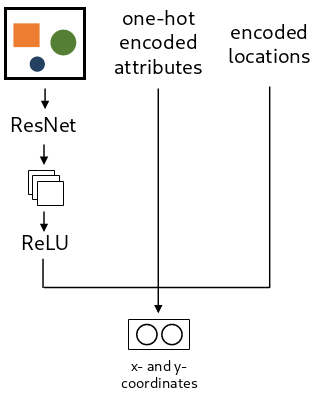
\includegraphics[width=0.35\linewidth]{figures/arch_coordinate_predictor.png}
        \label{fig:coordinate_predictor_architecture}
    }
    \subfigure[Model including GRE description]{
        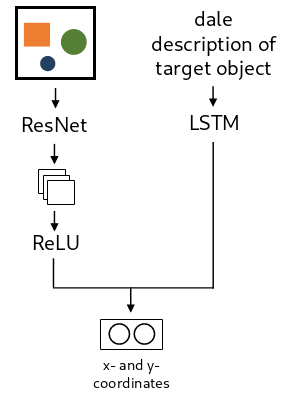
\includegraphics[width=0.315\linewidth]{figures/arch_coordinate_predictor_dale.png}
        \label{fig:coordinate_predictor_dale_architecture}
    }
    \caption{Simplified architecture of the coordinate predictors}
    % SD: How are these encoded?
    % DK: TODO
\end{figure}

In the first method, the target object is encoded as \textbf{one-hot encodings}, as described in section \ref{sec:object-identification}.
In an extension to this method, also the \textbf{center coordinates of all objects} in the image are included.
% SD: Encoded locations?
% DK: TODO
This should help the model to identify all possible options to chose from, when predicting the target object.
All the center coordinates are simply extracted and shuffled.
Since there are varying numbers of objects in the image, this vector of variable length is padded to the maximum number of objects in the dataset.
The padded locations consist of two zeros for both coordinates.
For both methods, the encodings of the target object are concatenated with the encoded image and then passed to the coordinate predictor.
% SD: Why shuffled? If we order them the way they appear in the image, the model will have more information that they are sequentially related.
% DK: TODO
% SD: Convolutions are only applied on visual features, not object attribute features and locations.
% DK: TODO

The third method encodes the attributes of the target object with human language using the \textbf{incremental GRE-algorithm}.
This opposes the idea described before, to share as few natural language information as possible with the model.
Still, this approach can help to understand and analyze if the model was able to extract information about the objects and more specifically their attributes from the image.
% SD: The question you are asking is whether it is possible to predict location from the visual appearance of the object. This is highly complex task as it requires quite two step reasoning, identification of features with that attribute, e.g. blue and then locating that feature in the image.
% DK: TODO
If the model is able to match parts of the image with human words it would show that the model learned this attribute.
If the model in a next step can learn this for the whole dataset, this would mean that it could generalize over these attributes and assign them to certain regions in an image.
This insight would help for succeeding models that make use of these learnings without human language.

% Using the algorithm, one can describe an object using its attributes to discriminate it from other objects as efficiently as possible.
% In other words, the object is described unambiguously using the lowest number of words.
% The algorithm assumes that there is an order of importance for attributes, such as shape, color and size.
% This order defines, which attributes can be left out, while still identifying the object uniquely.
% This research relies on the following order from most important to least important: shape, color, size
% Given for example the scene from \ref{fig:clevr-dale-5} with the target object being the \emph{big purple cylinder}.
% Using all three attributes, this description identifies the object perfectly and uniquely.
% Following the algorithm, we could make the description shorter by removing the least important attribute \emph{size} without loosing unambiguity, describing it as the \emph{purple cylinder}.
% This can be taken even one step further by removing also the \emph{color}.
% Describing it as the \emph{cylinder} still doesn't describe any distractor, since the target object is the only cylinder in the scene.
% % SD: See my point earlier about the reversed algorithm between the two tasks 
% % DK: TODO

For the experiments, each image is captioned with a description of the target object using the described algorithm.
To include it in the model, the captions need to be padded to an equal length.
In this case they are padded to a length of 3, which is the maximum number of attributes that can be used.
For this, as standard practice in captioning tasks, the captions are padded at the end with a specified padding token.

In the model, the referring expression is encoded, using an LSTM.
Here, the learned embeddings of each token are parsed by the LSTM and its final hidden state is then used as a summary of the complete caption.
Tokens are embedded with embedding dimensions $LSTM_e$ and the output of the LSTM has the size if $LSTM_o$.
The vocabulary that is used for the descriptions is based on 14 symbols, including the padding token.
Both the processed image and the final hidden state of the LSTM are flattened and concatenated, which is then passed through the coordinate predictor.
% SD: \citep and \citet Use Name (year) when you are referring to particular person and (Name, year) when you are referring to a paper. Hence, in this case it would be the latter.
% DK: done

The fourth method, to encode the target object utilizes \textbf{masking} of the image.
% SD: Oh, before we talked about 3 methods
% DK: done
The image is masked in the same way as in section \ref{sec:referring_expression_generation}.
While even the one-hot encodings contain human knowledge by explicitly encoding human chosen attributes, masking the image will only point the model towards the target object without giving more information.
It therefore can only rely on its own extracted visual features and the inherent human bias in the image when looking at masked images.
% SD: The information in the masked image is still not enough to identify the precise location, only the region. Hence, it corresponds on attention in the attention models. But those are generating labels and not predicting coordinated. The task is still challenging.
% DK: TODO
Both original and masked image are processed as described in \ref{sec:image-processing} and afterwards passed through the coordinate predictor.

For all setups, the same hyperparameters as in the previous experiments are used: a learning rate of $2\times10^{-4}$, a batch size of 32 samples and 30 epochs, \emph{Adam} \citep{Kingma2015} as optimizer.
8000 randomly selected samples are used for training, the remaining 2000 samples for testing.
The loss is calculated using cross entropy.
Table \ref{tab:variables-reference-resolution} shows the variables that are changed during the experiments for each of the models.

\begin{table}[ht]
    \centering
    \begin{tabular}{lcccc}
        \toprule
                               & $e_i$              & $c$               & $LSTM_e$  & $LSTM_o$               \\
                               & $[100, 500, 1000]$ & $[512,1024,2048]$ & $[15,30]$ & $[500,1000,1500,2000]$ \\\midrule
        reference resolver     & \times             & \times            & -         & -                      \\
        + one-hot              & \times             & \times            & -         & -                      \\
        + one-hot + locations  & \times             & \times            & -         & -                      \\
        + referring expression & \times             & \times            & \times    & \times                 \\
        + masking              & \times             & \times            & -         & -                      \\
        \bottomrule
    \end{tabular}
    \caption{Variables for each model where $e_i$ is the image embedding dimension, $c$ the dimensions of the coordinate predictor, $LSTM_e$ the embedding dimensions for tokens in the LSTM and $LSTM_o$ the output dimension of the LSTM}
    \label{tab:variables-reference-resolution}
\end{table}

The test dataset is again evaluated on the euclidean distance of the predicted coordinates to the ground truth coordinates.
This distance needs to be minimized.
The mean of all calculated distances is calculated across the whole epoch, which results in a mean distance score per epoch.
Since this score only takes the average of all predictions into account it doesn't show how every prediction fared individually.
If for instance the prediction of one object is getting more precise with growing number of epochs, but the precision of another object gets worse, the mean distance will stay the same.
% SD: Yes that’s correct but through several epochs we hope we will refine the distance and standard deviation of the error. It should level out. It is not a problem. What you do with a circle and accuracy is that you make the task easier as your pointer is now not pointing to a point but to a larger area.
% DK: TODO
It doesn't reflect this change.
For that reason, we also introduced an accuracy score.
For that we defined a fixed size circle with a radius of 20 pixels around the center of each object.
If the model's prediction lies in this circle, it will be counted as a correct prediction, if it lies outside, it is a false prediction.
These scores are averaged for the epoch and result in an accuracy score, where 100\% means that all predictions were very close to the center coordinates and 0\% means that no predictions were close to the center coordinates.
% SD: But here the score will face the same problem with steward deviation. Hence the only difference here is that pointing is less precise.
% DK: TODO
This of course doesn't give a perfect representation since the size of the objects varies, but it will still show, how precise each individual prediction is.
A high accuracy may indicate that the model could identify this specific object better.

The reference resolution models are trained on the 'CLEVR single' as well as on both 'Dale' datasets.
The 'CLEVR single' dataset should test the model if it can actually learn locations of an object.
Since the model relies on the extracted features of either VGG or ResNet, locational information about the image could have gone lost.
% SD: Explain. w3 had a paper with John Kelleher on what spatial information is encoded in CNNs
% DK: TODO
Training on this dataset should make sure that the model can converge towards the correct pixels, utilizing these features.
In a next step, the 'Dale' datasets provide the actual problem of discriminating objects from each other and afterwards pointing to the correct one.
Here, the models should make use of the additional given referring expressions about the scene, as one-hot encodings of the attributes, descriptions using the GRE-algorithm or the encoded locations.
'Dale-2' and 'Dale-5' provide two different difficulties for the model, where it needs to discriminate a target object from one or four distractors.
% SD: Point at not just discriminate
% DK: TODO
Latter task is assumed to be significantly harder.

\subsubsection*{Results}

\begin{figure}[ht]
    \centering
    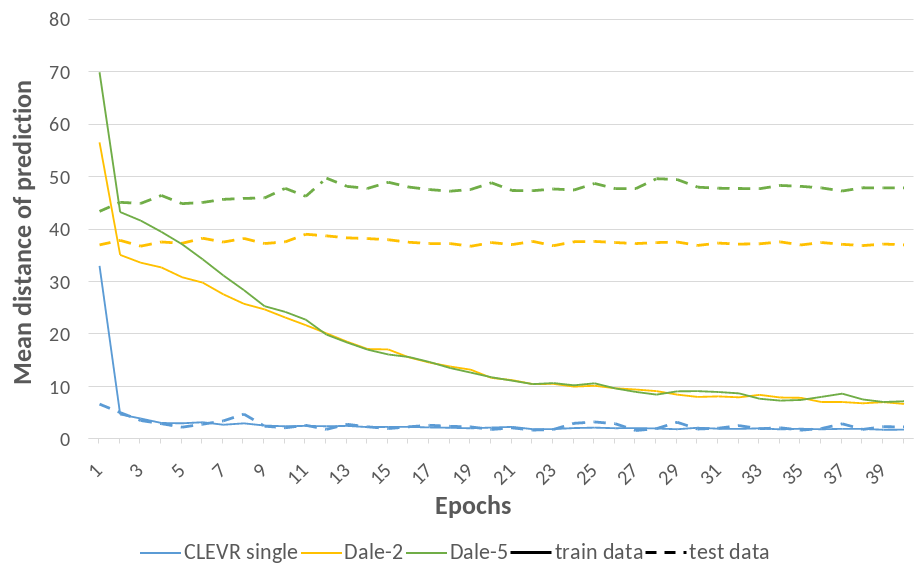
\includegraphics[width=0.8\linewidth]{figures/coordinate-predictor_loss.png}
    \caption{Mean distance between predicted coordinates and ground truth in pixels on different datasets}
    \label{fig:coordinate-predictor_loss}
\end{figure}

Figure \ref{fig:coordinate-predictor_loss} shows the results of the coordinate predictor that doesn't include any information about the target object.
The used feature extractor for these results is \emph{Resnet-3}, but the results don't differ meaningfully from results with other feature extractors.
As can be seen, the success between the different datasets are significant.
The more objects are present in an image, the worse the model performs.
The model converges for the CLEVR single dataset after around 20 epochs to a mean distance of around 2 pixels.
This prediction even though not perfectly on the center point is always on the object.
Opposed to that, using the Dale-2 dataset with two objects, the mean distance lies between 37 and 38 pixels already after the first epoch and doesn't drop with increasing number of epochs.
With five objects in the Dale-5 dataset, the model only predicts a mean distance of around 45 pixels in the beginning, which worsens with a rising number of epochs to 48 pixels.

An interesting observation is the difference of the mean distances between training and testing data.
% SD: How can we have epochs on the testing data? There is no updates so i5 does not make sense.
% DK: TODO
The training distance is constantly approaching zero, while the testing loss is staying constant or even getting higher.
This points to the fact that the model is not generalizing the task by learning abstract patterns that can be applied to unseen data, but is instead memorizing the training data.
That is especially visible for the Dale-5 dataset, where learning the patterns of the training data looses even the ability to interpret some patterns in the testing data.
Applying a higher dropout didn't have an impact on the results.
% SD: The results show that the model is learning something from the training data but this is not the feature that should be learning as the performance on the test data is low. Actually, is it low, it is 10, 35 and 45 pixels. We should not expect any difference between epochs as there is no training. Hence, a flat line is expected.
% DK: TODO

This behavior is indeed not very surprising.
First, results with the 'CLEVR single' dataset show that the model is able to derive geometrical information from abstract feature, extracted by a feature extractor.
Geometrical information therefore doesn't get lost during this abstraction, but the model is able to point to a specific object, as long as only one object is part of the image.
% SD: Because it is in the same location?
% DK: TODO
Secondly, more than one objects present in an image confuses the model, and it is not able to consistently point to one of them.
This can have multiple reasons, for instance that the models lacks the ability to separate objects in the extracted features.
But even in case, the model is able to do that and could determine the location of each object in the scene given the feature, it would not be able to tell, which of these is the actual target object.
The guess is then more or less random.
This especially applies to the Dale-2 dataset, where an identification of the target object just based on one distractor is impossible; both of the present objects are unique.
For the Dale-5 dataset, the model could in theory learn that the target object is always the one object which is unique in respect to its and the distractors' attributes.
This task on the other hand seems very difficult to learn.
In conclusion, the models are able to predict geometrical coordinates, but need more information about the target object to identify it.

When the target object \textbf{attributes are encoded as one-hot vectors} and added to the input, the results don't improve.
One factor that now has a much higher impact is the feature extractor that is used.
Table \ref{tab:feature-extractor-mean-distances} compares the mean distances the models predict for the different feature extractors.
The results are shown for the models trained on the Dale-2 and Dale-5 datasets for training and test data.
First, a big difference can be seen between the datasets.
The models only converge to a minimum mean distance of around 46 pixels to the correct coordinates for the Dale-5 dataset, looking at the test data.
In most cases, it stays above 50 pixels.
% SD: What is the image size? What is the size of a typical object? 50 sounds quite good. Attention is predicting one of 7x7 blocks. Is 50 more or less than 1/7 of an image? 
% DK: TODO
Using the Dale-2 dataset, the behavior is a little different.
All ResNet extractors with four residual blocks and an additional average pooling and optionally a classifier layers reach similar scores as the experiments before without any one-hot encodings.
Interestingly, without the classifier layer, the model doesn't converge at all and the mean distances jump up and down between the epochs.
This effect also applies when using less residual blocks.
Using the VGG, only VGG-cls2 achieve a similar performance, while the others predict coordinates between 43 and 46 pixels away.

\begin{table}[ht]
    \centering
    \begin{tabular}{rcccc}
        \toprule
                            & \multicolumn{2}{c}{\textbf{Dale-2}} & \multicolumn{2}{c}{\textbf{Dale-5}}                                   \\\cmidrule(lr){2-3}\cmidrule(lr){4-5}
                            & train                               & test                                & train          & test           \\\midrule
        \textbf{VGG-0}      & 30,27                               & 46,20                               & \textbf{32,17} & 54,40          \\
        \textbf{VGG-avg}    & \textbf{29,99}                      & 45,08                               & 32,32          & 52,67          \\
        \textbf{VGG-cls1}   & 37,99                               & 43,28                               & 46,57          & 50,75          \\
        \textbf{VGG-cls2}   & 38,87                               & \textbf{39,02}                      & 47,48          & 49,91          \\
        \textbf{VGG-cls3}   & 39,99                               & 44,32                               & 47,26          & \textbf{46,77} \\\midrule
        \textbf{ResNet-3}   & 78,26                               & 65,23                               & 92,07          & 91,12          \\
        \textbf{ResNet-4}   & 44,14                               & 55,24                               & \textbf{36,48} & 58,28          \\
        \textbf{ResNet-avg} & \textbf{33,06}                      & \textbf{39,18}                      & 47,64          & 46,38          \\
        \textbf{ResNet-cls} & 37,57                               & 38,10                               & 44,72          & \textbf{45,92} \\
        \bottomrule
    \end{tabular}
    \caption{Mean test losses for different feature extractors with one-hot attribute encodings after 20 epochs}
    \label{tab:feature-extractor-mean-distances}
    % SD: Explanation of labels
    % DK: TODO
\end{table}

Secondly, the training loss now looks also different.
In almost no cases, the models converge to a lower mean distance than with the test data, meaning a higher precision in their predictions, as they did in the experiment before.
The only exception is ResNet-3 as a feature extractor.
In other words, the models are again not able to generalize, but in specific cases memorize the patterns in the train data.
This hints to the fact that only specific layers of the feature extractors contain information that is generally usable to identify and discriminate objects.
Especially the lower layers with fewer residual blocks in the case of ResNet and no classifier layers for the VGG seem to not encode knowledge that can be utilized for this task.
Higher layers, with more specific encoded information need to be used for this research.
The experiments in the following sections are set up using these higher layers.

Adding \textbf{information about the center coordinates} of all objects should have helped the models to get a list of possible predictions.
In theory, the model could learn to choose between these coordinates by relating them to the extracted features of the image.
This hypothesis doesn't hold.
All results for both datasets Dale-2 and Dale-5 are the exact same as without included information about the locations.
The problem therefore doesn't seem to lie in predicting coordinates in general, but predicting the coordinates of the target object.
% SD: Perhaps arranging the objects sequentially would help the model learn spatial contiguity, see my earlier comment.
% DK: TODO
The model is still not able to understand, which object is the target object.
For that reason, a better representation of the target object is necessary.

In a next step, information about the attributes is included using the \textbf{\emph{GRE-algorithm}} from \citet{Dale1995}.
Again, the mean distance of the predictions as well as the accuracy doesn't improve compared to the previous experiments.
% SD: Table with these results?
% DK: the table would show the same figures as the existing table. Should be still included? (QUESTION)

\begin{figure}[ht]
    \centering
    \subfigure['Dale-2', train split]{
        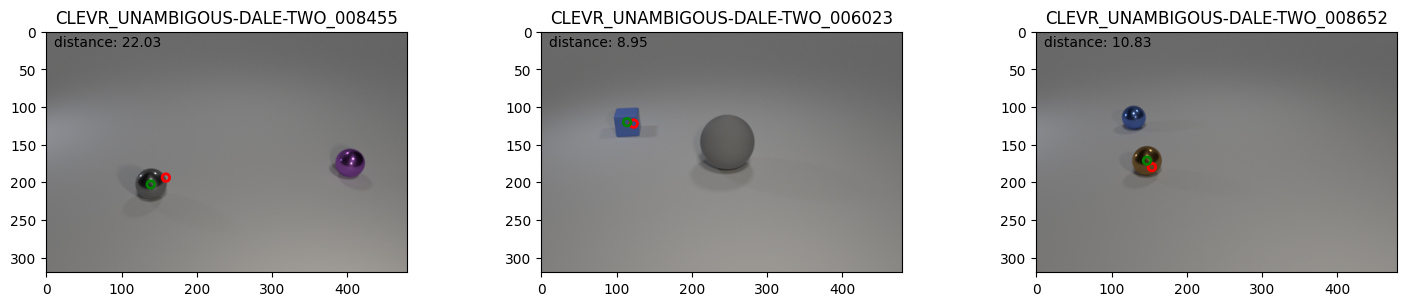
\includegraphics[width=.92\linewidth]{figures/visualization_dale-2_train.png}
        \label{fig:visualizations_dale-2_train}
    }
    \subfigure['Dale-2', test split]{
        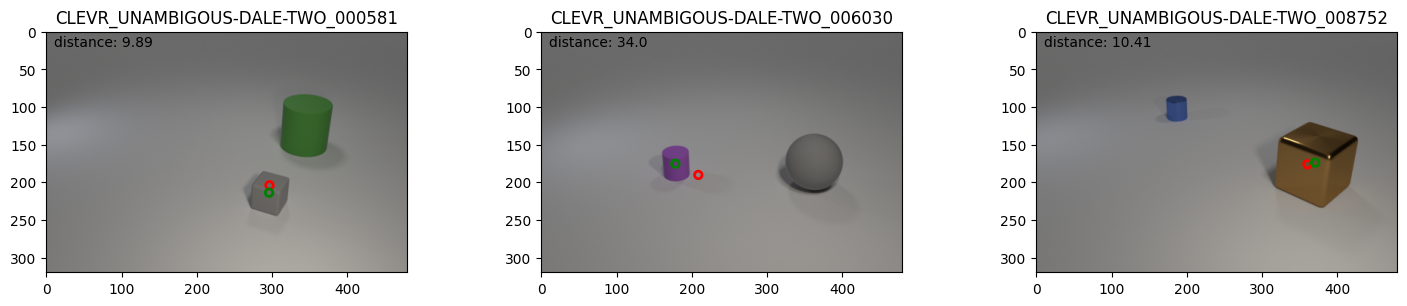
\includegraphics[width=.92\linewidth]{figures/visualization_dale-2_test.png}
        \label{fig:visualizations_dale-2_test}
    }
    \subfigure['Dale-5', train split]{
        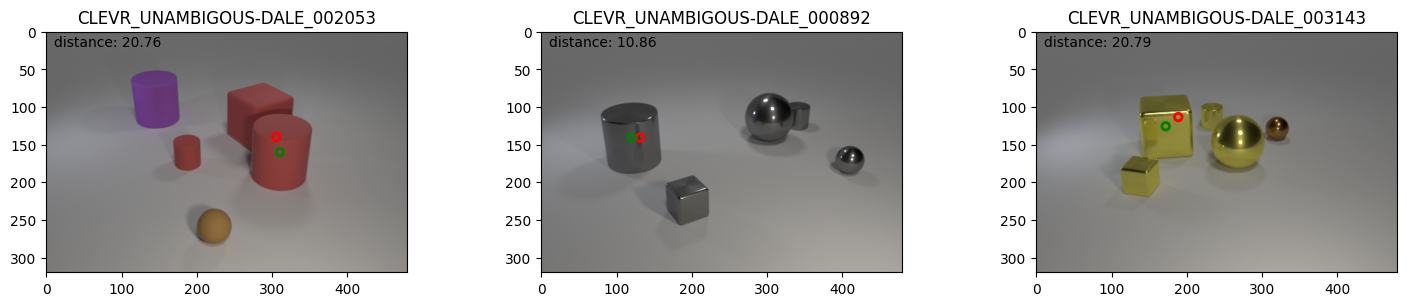
\includegraphics[width=.92\linewidth]{figures/visualization_dale-5_train.png}
        \label{fig:visualizations_dale-5_train}
    }
    \subfigure['Dale-5', test split]{
        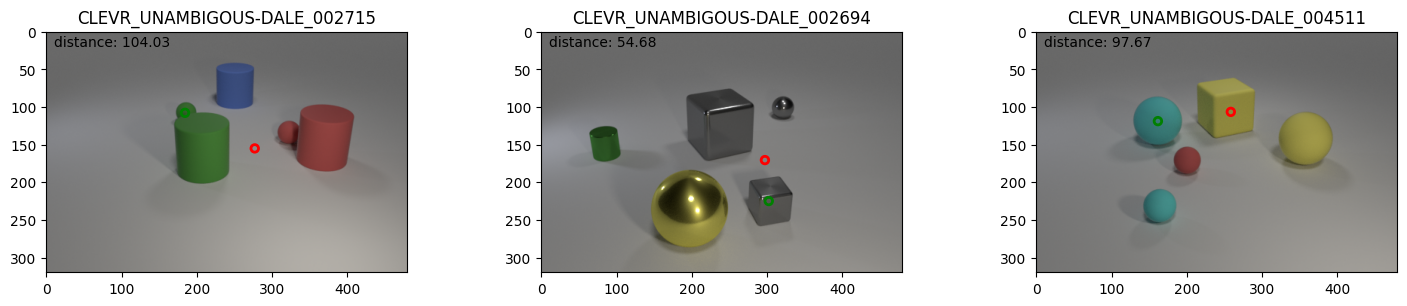
\includegraphics[width=.92\linewidth]{figures/visualization_dale-5_test.png}
        \label{fig:visualizations_dale-5_test}
    }
    \caption{Visualization of the models' predictions in the 'Dale' datasets}
    \label{fig:visualizations_dale}
\end{figure}

An interesting pattern appears when doing a qualitative analysis of the models' predictions.
Here, we visualized the predicted coordinates compared to the ground truth coordinates.
Figure \ref{fig:visualizations_dale-2_train} shows random examples of predictions for images in the train dataset of Dale-2.
The green circle shows the ground truth center coordinates of the target object, while the red circle shows the prediction of the model.
As can be seen, the predictions are very precise.
Figure \ref{fig:visualizations_dale-2_complete_train} combines the predictions and ground truths across all images in the train dataset.
This shows general patterns of the models predictions over the complete dataset.
Here, all predicted coordinates are placed as red circles into the image, while all ground truth coordinates are placed as green circles.
The resulting shape is a rhombus, which reflects that all objects are placed usually central into the scene.
As expected the green and red rhombus align mostly in the same area for the train split of the 'Dale-2' dataset.
% SD: But this image does not show clearly whether the circles for the same object match. You could calculate the average error in distance between the ground truth and predicted coordinates.
% DK: that is done in the quantitative analysis (mean square error above). The visualization should show general learned patterns of the model (as in this case predictions toard the center)

The results look very different for the test split.
As can be seen in Figure \ref{fig:visualizations_dale-2_test}, the three randomly selected predictions don't align with the ground truth coordinates.
For all the images, the predictions don't lie on any object.
In the left image as well as in the central image, the predictions are closer to the target object than towards the distractor, but are still quite imprecise.
% SD: They are closer to the target than distractor and you can see that it is working to a point. But remember this task is very challenging and I wouldn't say the results are so negative.
% DK: right, this is addressed in the conclusions below
These findings align with the mean distance scores, described in the sections before.
However, it seems that the model's predictions are all towards the center of the image.
This can be seen clearer in Figure \ref{fig:visualizations_dale-2_complete_test}.
Again, the green circles form the shape of rhombus.
In contrast, the predictions in red almost all cluster in the center of the image.
They form roughly the shape of a smaller rhombus.
% SD: There is a bias towards the centre but I would not say that the model has not learned anything. I'm surprised that it works so well given the feature representation we have, i.e. no geometric features.
% DK: again, conclusion below
This behavior can be observed for all datasets and architectures of the model.
Figures \ref{fig:visualizations_dale-5_train}, \ref{fig:visualizations_dale-5_test}, \ref{fig:visualizations_dale-5_complete_train} and \ref{fig:visualizations_dale-5_complete_test} show the results for the 'Dale-5' dataset.
Here, the model more likely predicts the center coordinates of a distractor object as seen in the right image, which is also reflected in the lower score of the mean distance.
Also the combined visualization shows the same clustering of predictions in the center of the scene, but the pattern of the smaller rhombus is more visible.
% SD: The centre bias could be the way the error function is used, that is averages all distances and of course this has a tendency to some middle distance. A solution would be to have better geometric features that could take these errors better into account.
% DK: TODO (future work)

\begin{figure}[ht]
    \centering
    \subfigure['Dale-2', train split]{
        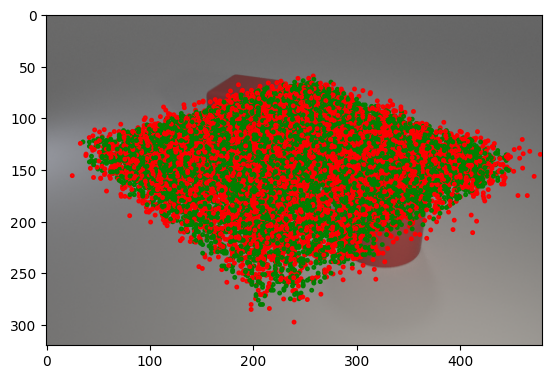
\includegraphics[width=0.42\linewidth]{figures/visualization_dale-2_train_complete.png}
        \label{fig:visualizations_dale-2_complete_train}
    }
    \subfigure['Dale-2', test split]{
        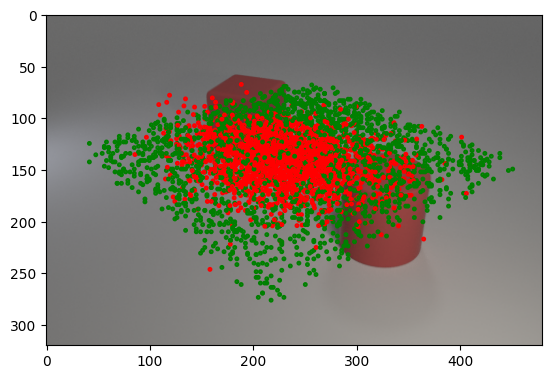
\includegraphics[width=0.42\linewidth]{figures/visualization_dale-2_test_complete.png}
        \label{fig:visualizations_dale-2_complete_test}
    }
    \subfigure['Dale-5', train split]{
        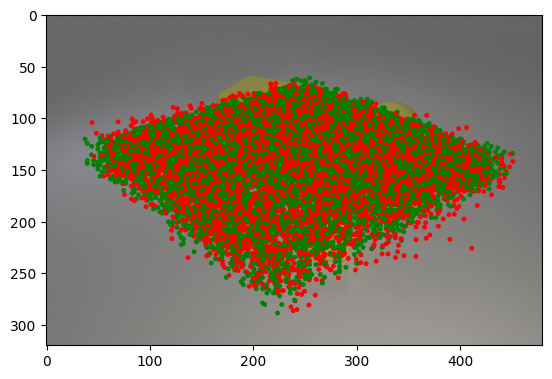
\includegraphics[width=0.42\linewidth]{figures/visualization_dale-5_train_complete.png}
        \label{fig:visualizations_dale-5_complete_train}
    }
    \subfigure['Dale-5', test split]{
        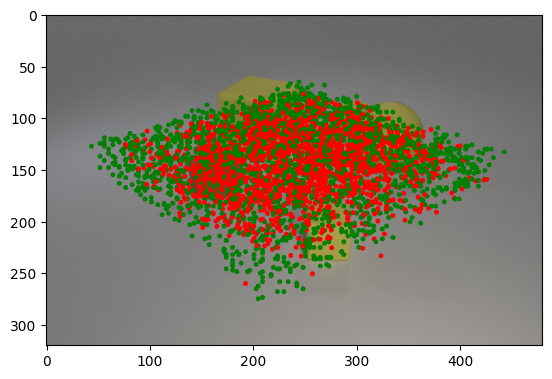
\includegraphics[width=0.42\linewidth]{figures/visualization_dale-5_test_complete.png}
        \label{fig:visualizations_dale-5_complete_test}
    }
    \caption{Visualization of the models' predictions in the Dale datasets}
    % SD: I Haven't checked the earlier captions, but the captions should be informative in the sense that one does not need to look for the text to understand them. Hence, include a brief summary of what each figure contains.
    % DK: TODO
    \label{fig:visualizations_dale_complete}
\end{figure}

These results allow two conclusions.
First, the models are biased to predict coordinates in the center of the image.
% SD: centre - using British English?
% DK: so far I used always American English (hopefully consistently)
The reason for this is likely that the model can produce a relatively low loss, without relying on many extracted features of the objects.
Since all objects are always located in the center of the image and never in its corners, a prediction of any coordinate in the center is on average closer to the target object than any random prediction or predictions of coordinates at the borders of the image.
The model therefore learns only, where any object is likely located and can minimize the mean distance to a certain extent with this strategy.

Second, even though the models are biased towards the center of the image, the predictions are still often leaning towards the location where many objects lie.
This can be seen for the 'Dale-5' dataset, especially in left and central image in Figure \ref{fig:visualizations_dale-5_test}.
Again, by this strategy, the model can minimize the mean distance, since the probability is high that the target object lies in this cluster of objects.
Concluding, the model is able to extract, where objects are located in the image, but can't make use of the referring expressions, to decide which of these objects is the target object.
% SD: There is a centre bias and the model can partially locate the target. The task is hard. The features are not optimal for this task. Future would should focus on using geometric features - we should have tried these and I'm sure we would get better results. Another extension would be making pointing less precise, i.e. focus on a single point, i.e. using a circle of 20 pixels or a 7x7 grid as in the attention mechanism. This would simplify the task.
% DK: TODO (future work)

\newpage

\section{Language games}
\label{sec:language-games}

The experiments that are executed using language games have a similar structure as the experiments in the previous chapters, since those provided the basis for the language games.
% SD: But there is an importnat difference that now we have two neural netweorks, the sender and the receiver.
% DK: TODO

The language games in this research have an asymmetric setup.
One agent, the sender is shown some information and needs to generate a message.
This message is received by the second agent, the receiver.
The receiver needs to parse this message and combine it with the same information that the sender was presented with.
The receiver then makes a prediction, which is compared to the ground truth.
The game is set up prosocial, which means that both agents receive the same loss based on the receiver's prediction.
All weights of the agents are adapted in the same way.

The vocabulary that the sender can draw from to produce a message is made up of initially arbitrary symbols.
The meaning of these symbols is created as soon as the sender uses them in one of the message, and the receiver is able to use it to solve the task successfully.
Over time, specific meanings are reinforced and a language emerges.
The number of possible words, namely the size of the vocabulary can be varied.
% SD: But possibly you would describe the language game setup already before on the background or method chapter. I would move all text there and make the language games description much more detailed, also giving examples. What is happening in terms of interaction? How is this modelled with the neural networks? It is important to emphasise this difference.
% DK: TODO

First, we will discuss \emph{discrimination games}, because they have the simplest setup.
% SD: What is this setup?
% DK: TODO
Furthermore, other language games that research this topic use a very similar setup.
In the next step, we will describe \emph{caption generators} that are set up as a language game.
Here, the sender describes the scene, while the receiver needs to generate a caption.
In the last step, we try to lose as much human bias as possible and the models are trained on just 'pointing' towards the target object, by again predicting its center coordinates.
% SD: Why are we not testing it on all 3 games?
% SD: Not sure what you mean here? Why do we loose human bias? 
% DK: TODO

The languages that emerge are analyzed in two ways.
An analysis of the frequency of used symbols and messages, as well as an examination for which images and objects they are used indicates the structure of the language and meanings of the symbols.
In a second step, the language is compared to several referring expressions in natural language.
By doing this, it can be seen if the models learned to use similar ways of referring to objects as humans do, or if they rely on different approaches.

\subsection{Object identification}
\subsubsection*{Setup}

In a discrimination game, the agents are presented with two or more images, one of these being the target image.
The sender needs to communicate this target image to the receiver by discriminating it from the other distractor images.
The receiver then needs to decide based on the message, which of the images is the target image.

The discrimination games in this research have a very similar setup as described in \citep{Lazaridou2017}.
The agents in this research resemble their \emph{agnostic sender} as well as their \emph{receiver}.
One central difference is the production of the message.
The main goal of their language game was the identification of the concept that and image was related to.
Therefore, the sender communicated only single-symbol messages to the receiver, which should describe the concept of the target image.
Opposed to that in this research, the agents are tasked to discriminate objects from each other based on their attributes.
% SD: On the contrary,...
% DK: TODO
It is therefore assumed that the sender will communicate these discriminative attributes.
For that reason, the sender is allowed to generate sequences as a message.

Both 'Dale' datasets are used to train the agents in this mode.
Similarly to the bounding box classifier, bounding boxes around each of the objects are extracted and fed to the game.
As in \citep{Lazaridou2017}, the sender receives the bounding box of the target object as the first image, while the rest of the bounding boxes are shuffled.
% SD: Here it does not receive a boundig box of an object as in Lazaridou. They use whole images, don't they?
% DK: TODO
The sender is assumed to learn which of the input images is the target images by this approach.
The receiver receives the images in completely shuffled order.

\begin{figure}[h]
    \centering
    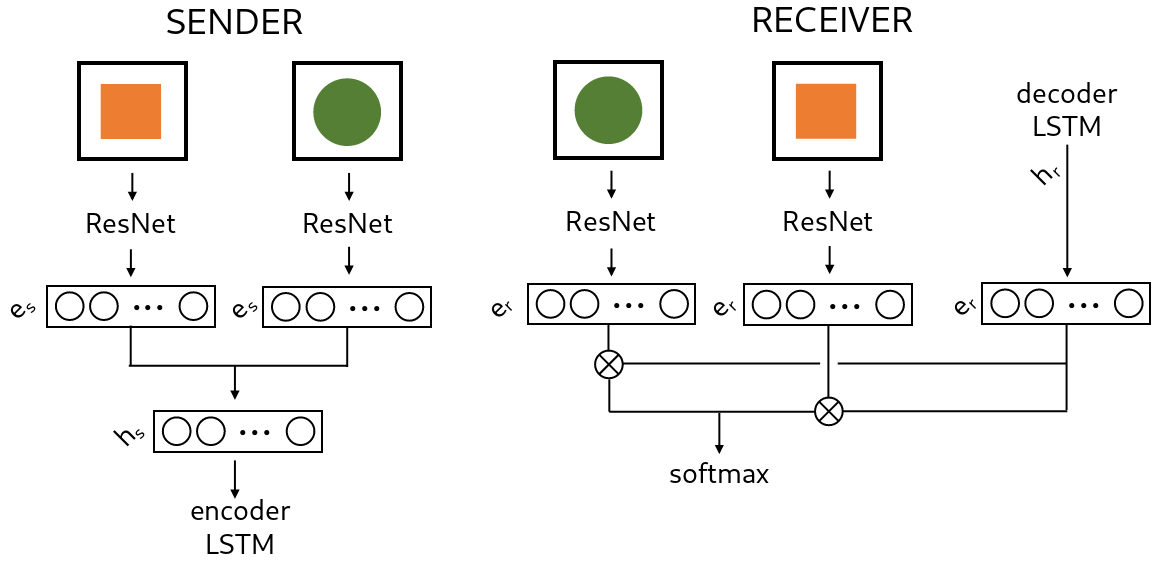
\includegraphics[width=.8\linewidth]{figures/arch_discriminator.png}
    \caption{Sender and receiver architectures in the discrimination game}
    \label{fig:discriminator_architecture}
\end{figure}

Figure \ref{fig:discriminator_architecture} shows, how the sender and the receiver of the discriminator are built up.
For the sender, the images are passed through a feature extractor and a following linear layer that reduces the dimensions to an embedding size $e_s$.
All embedded images are concatenated and passed through another linear layer to reduce the dimensions to the hidden size $h_s$.
This is then used as the initial state of the encoder LSTM in the sender wrapper.
% SD: Deatils about the layers, their parameters. More explanatory figure caption.
% DK: TODO

The receiver also encodes all images using a feature extractor with a following linear layer, reducing it to $e_r$.
The sequence, received by the sender is the input for its decoder LSTM, where the hidden state with a dimension of $h_r$ is randomly initialized.
As mentioned above, the receiver combines this image representation with the hidden state of each symbol separately.
This is done by passing the hidden state through a linear layer to scale its dimensions to the same $e_r$.
This allows the calculation of the dot product between it and the image representation.
If the message describes an object well, the resulting dot product should be higher.
The receiver then `points' to one of the images by applying the \emph{softmax} function over the results of the dot products.
The loss is calculated using the NLL-loss.

During the experiments, five variables are adjusted to compare their effects:
(1) the image embedding size for the sender $e_s$, (2) the LSTM hidden size for the sender wrapper $h_s$, (3) the image/message embedding size for the receiver $e_r$, (4) the LSTM hidden size for the receiver wrapper $h_r$ and (5) the size of the vocabulary $|V|$.

\subsection*{Results}
Table \ref{tab:results_discriminator} shows the accuracy of the models calculated on the success of communication if the receiver can identify the target object.
A random guess corresponds to 50\% in the \emph{Dale-2} dataset and 20\% in the \emph{Dale-5} dataset.
Four different vocabulary sizes $|V|$ are tested.
A size of 13 symbols corresponds to the 13 attributes the objects can have and align with human language.
If the symbols were similarly used, messages would have lengths between one and three symbols.
Opposed to that a slightly smaller vocabulary with 10 symbols is used to create a smaller bottleneck with a higher pressure to condense the information.
Similarly, a bigger vocabulary consisting of 20 symbols tests how a bigger bottleneck changes the results.
Lastly, a big vocabulary of 100 symbols should give the model all options to encode the information, including one symbol per attribute or one symbol describing a combination of attributes.
% SD: Motivation why this is so. The possible number of strings is {#colour} x {#shape} {object type} where all numbers except the last one also contain a padding token.
% DK: TODO

The hidden sizes $h_s$ and $h_r$ as well as the embedding sizes $e_s$ and $e_r$ are chosen in alignment with the vocabulary size.
The hidden sizes are always smaller or equal to the vocabulary size since the information about each word needs to be compressed in a smaller dimension to learn meaning.
Hereby, hidden sizes of 10 and 100 are tested.
On the other hand, three different embedding sizes are tested: 10, 50 and 100.
The reason for this is to experiment, what is the optimal middle ground between compressing features of an image encoded in high dimension vectors and upscaling encoded messages in low dimension vectors.
% SD: This discussion of dimensions could already be introduced when you discuss simple modles earlier as the same dimensions are used. This is a more an evaluation of represnetations rather than interaction and hence it would fit there.
% DK: TODO

\begin{table}[h]
    \centering
    \begin{tabular}{ccccc|cc|cc|cc}
        \toprule
              &         &         &         &         & \multicolumn{2}{c}{\textbf{Dale-2}} & \multicolumn{2}{c}{\textbf{Dale-5}} & \multicolumn{2}{c}{\textbf{CLEVR color}}                                                         \\\cmidrule(lr){6-7}\cmidrule(lr){8-9}\cmidrule(lr){10-11}
        $|V|$ & $h_{s}$ & $h_{r}$ & $e_{s}$ & $e_{r}$ & \textbf{Accuracy}                   & \textbf{length}                     & \textbf{Accuracy}                        & \textbf{length} & \textbf{Accuracy} & \textbf{length} \\\midrule
        {10}  & {10}    & {10}    & {10}    & {10}    & {96,4\%}                            & {0,99}                              & {24,7\%}                                 & {0}             & {17,3\%}          & {1}             \\
        {10}  & {50}    & {50}    & {50}    & {50}    & {50\%}                              & {1}                                 & {21,4\%}                                 & {1}             & {17,8\%}          & {0}             \\
        {13}  & {10}    & {10}    & {10}    & {10}    & {96,16\%}                           & {1}                                 & {24,8\%}                                 & {1}             & {17,1\%}          & {1}             \\
        {13}  & {10}    & {10}    & {50}    & {50}    & {49,6\%}                            & {1}                                 & {21,9\%}                                 & {1}             & {17,9\%}          & {0}             \\
        {20}  & {10}    & {10}    & {50}    & {50}    & {50,9\%}                            & {0}                                 & {23\%}                                   & {1}             & {15,9\%}          & {1}             \\
        {100} & {10}    & {10}    & {10}    & {10}    & {97,3\%}                            & {1}                                 & {24\%}                                   & {1}             & {18,1\%}          & {1}             \\
        {100} & {10}    & {10}    & {50}    & {50}    & {49,9\%}                            & {1}                                 & {24,4\%}                                 & {1}             & {15,8\%}          & {1}             \\
        {100} & {100}   & {100}   & {100}   & {100}   & {49\%}                              & {0}                                 & {25,3\%}                                 & {1}             & {15,6\%}          & {0}             \\
        \bottomrule
    \end{tabular}
    \caption{Results of the discriminators: $|V|$ are different vocabulary sizes, $h$ hidden sizes and $e$ embedding sizes.}
    % SD: A note about the datasets chosen. Why do we choose these? Initially, we describe more than 3 datasets.
    % DK: because the 'CLEVR Single' contains only one object. So there is nothing to discriminate (done)
    \label{tab:results_discriminator}
\end{table}
% SD: As we discussed at Semdial, it would be good to have a learning curves here that would show how fast or slow the languages converge. As David pointed out it may be that convergence is unstable and changes happen in between.
% DK: TODO

For the \emph{Dale-2}, a clear correlation between the hidden sizes, embedding sizes and the size of the vocabulary can be identified.
A hidden/embedding size as high as the vocabulary size is beneficial for identifying the correct object.
The receiver identifies almost every sample correctly when all sizes are 10.
When the hidden and embedding sizes are increased, the guesses by the receiver are random with 50\% accuracy.
Interestingly, a vocabulary size of 10 is enough to communicate a meaningful message when the model is trained on the \emph{Dale-2} dataset.
% SD: How do we know? What would happen if the hidden layers are smaller than the vocabulary size? We would also need to test several smaller dimensions.
% DK: because the task is solved succesfully, TODO

The results change, when using the \emph{Dale-5} dataset with four distractors.
With four distractors and with low hidden, embedding and vocabulary sizes, the agents barely pass the random baseline with 23\%.
Only increasing the vocabulary size to 100 raises the accuracy by almost 20\% points to 43\%.
This is still considerably lower than the 95\% of the \emph{Dale-2} dataset.
The same applies to the 'CLEVR color' dataset, where all models achieve a very low accuracy of around 15 to 17\%, corresponding to random guesses.
% SD: Could we say that calculation on Dale-5 is successful?
% DK: TODO

Two conclusions can be drawn.
First, the hidden as well as the embedding sizes need to be close to the vocabulary size.
% SD: Not sure, since we never tested smaller layer sizes. If the embedding layers are the same as the vocabulary size then at least a language encoding LSTM is not motivated to geenralise at all as it can keep representations for individual words without abstracting them. Leanring word embeddings involves reducing dimensions.
% DK: TODO
This even applies for very low vocabulary sizes, which means that the image encodings need to be compressed to the same low dimensions.
The reason for this is very likely that neural models have difficulties to upscale from lower dimensions (e.g. from low $h_r$ to high $e_r$) as opposed to learn how to extract the important information from a vector with many dimensions.
% SD: Hypothesis space to find the target function is just too big and they can never approximate that function.
% DK: TODO

The second conclusion that can be drawn looks at the differences between the two datasets.
Unsurprisingly, the agents have a much higher difficulty to discriminate a target object from four instead of one distractor.
Since we discriminate objects based on properties that are also distinguished in human cognition (8 colors, 2 sizes, 3 shapes), we expect that the vocabulary onto which the agents converge reflects these categories and is therefore close to human vocabulary.
There are $8*2*3=48$ possible combinations of attributes.
% SD: Calculation behind this figure?
% DK: (done)
Still, for Dale-2, a vocabulary size of only 10 is enough for an almost perfect accuracy with two objects.
This hints to the fact that the agents don't describe the complete target object, but only rely on discriminative attributes between the objects.
The need for a more detailed description of discriminative attributes is higher when more distractors are involved.
Therefore, the models need to learn more combinations of symbols in order to attest to this higher level of detail and especially how to relate them to features in the images.
% SD: We would need to show that the messages in Dale-2 are shorter than in Dale-5 to claim this.
% DK: TODO

\cmtDK{similarity to bounding box classifier}

\subsection{Referring expression generation}
\subsubsection*{Setup}

In a next step, it is tested if the agents can learn to extract features of the objects together.
For this, the receiver is tasked to describe the target object in natural language, while the sender needs to communicate, which object is the target.
Again, the setup is asymmetrical: the sender receives the image and information, which of the objects in the image is the target object in form of a masked image.
The receiver only sees the image without additional information.
\cmtDK{human bias vs emergent language}

This setup is based on the single neural model described above.
The target caption for each image is created using the GRE-algorithm of \citet{Dale1995}.
% SD: The sender uses the incremental algorithm?
% DK: TODO, QUESTION
Since the results of the experiments show that the position of the padding doesn't have an effect on the final converging scores, the padding tokens are only prepended to the caption.

\begin{figure}[h]
    \centering
    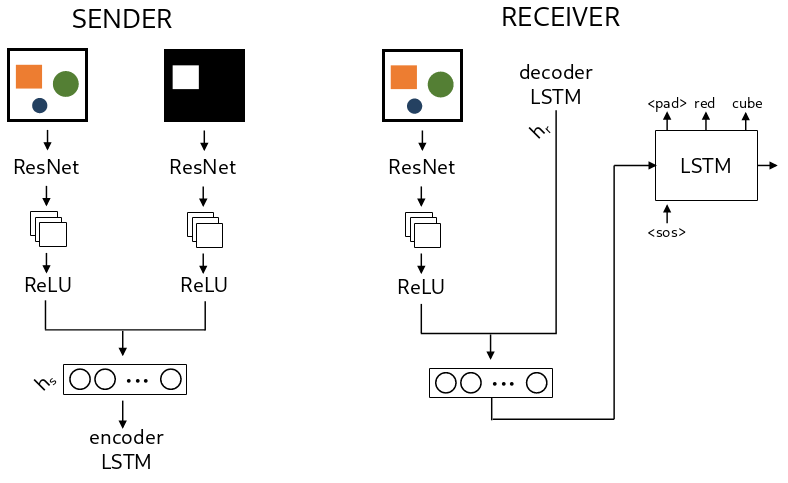
\includegraphics[width=.7\linewidth]{figures/arch_caption_generator_game.png}
    \caption{Simplified architecture of the caption generator game}
    \label{fig:caption_generator_game_architecture}
    % SD: But here we don't need an LSTM, we just want to identify one of the objects. The LSTM should only encode the inout message.
    % DK: TODO
\end{figure}

The sender is built up of two image encoders, one encodes the original target image and one encodes the masked image.
The image encoders are set up as described in \citep{Johnson2017}.
A feature extractor extracts basic features of the images.
Two following convolutional layers with a \emph{ReLU} function are trained to condense the most important information from the resulting matrices.
A max pooling layer and a linear layer reduce the dimensions to 1024 dimensions.
This size was found to have the best results during the experiments.
% SD: Reference back to when you reported this?
% DK: TODO
The two resulting encoded images are flattened and concatenated.
A final linear layer reduces this long vector to the hidden size of the message LSTM $h_s$, which is used as the initial hidden state of this LSTM.

The receiver uses the same architecture to encode the original image as the sender.
The resulting flattened vector is concatenated with the decoded message of hidden size $h_r$.
This is then passed through a linear layer, again reducing it to 1024 dimensions and is then used as the initial state of the captioning LSTM.
% SD: But receiver is not doing captioning? Is it incrementally identifying the objects as the sender's messages are coming in?
% DK: TODO
During training, the ground truth caption is used as the input to the LSTM using teacher forcing.
% SD: I'm not sure how teacher forcing is implemented, see my earlier comment
% DK: typo, teacher forcing is actually applied (done)
When presented with test data, the LSTM always produces three tokens, by using its own predicted words as the input for the next step.
The loss is calculated with cross entropy.

Since the agents are trained to describe the target object discriminatively based on the described GRE-algorithm, they are trained on the 'Dale-2' and 'Dale-5' dataset.
The 'Dale-5' should be again much harder to learn, since there are more objects that the agents need to discriminate the target object from.
% SD: So the sender is generating descriptions following the GRE policy?
% DK: TODO

During the experiments, the following variables are adjusted, and the results are compared:
(1) the vocabulary size $|V|$,
(2) the LSTM hidden size of the sender wrapper $h_s$ and
(3) the LSTM hidden size of the receiver wrapper $h_r$.
The same metrics as in the pre-experiments are used to evaluate the results.

\subsubsection*{Results}
\begin{table}[h]
    \centering
    \begin{tabular}{ccc|ccc|ccc}
        \toprule
              &         &         & \multicolumn{3}{c}{\textbf{Dale-2}} & \multicolumn{3}{c}{\textbf{Dale-5}}                                                                             \\\cmidrule(lr){4-6}\cmidrule(lr){7-9}
        $|V|$ & $h_{s}$ & $h_{r}$ & \textbf{Acc.}                       & \textbf{word-by-word}               & \textbf{length} & \textbf{Acc.} & \textbf{word-by-word} & \textbf{length} \\\midrule
        {10}  & {10}    & {10}    & {22,9\%}                            & {62,8\%}                            & {1}             & {7,1\%}       & {40\%}                & {1}             \\
        {13}  & {10}    & {10}    & {22,8\%}                            & {62,9\%}                            & {0}             & {7,3\%}       & {38,7\%}              & {1}             \\
        {20}  & {10}    & {10}    & {24,6\%}                            & {64\%}                              & {1}             & {6,7\%}       & {38,7\%}              & {1}             \\
        {100} & {10}    & {10}    & {24,4\%}                            & {62\%}                              & {1}             & {7,8\%}       & {40\%}                & {1}             \\
        {100} & {100}   & {100}   & {21\%}                              & {62\%}                              & {1}             & {6,5\%}       & {37,8\%}              & {1}             \\
        \bottomrule
    \end{tabular}
    \caption{Results of the caption generator: $|V|$ are different vocabulary sizes and $h$ hidden sizes.}
    % SD: What is word-by-word?
    % DK: the same as in the caption generator with a single model (QUESTION)
    \label{tab:results_caption_generator_game}
\end{table}

The results of the caption generator game are summarized in Table \ref{tab:results_caption_generator_game}.
In general, it can be seen that the agents have much bigger problems, to solve the task together than a single neural network.
The highest accuracy for descriptions, the agents manage to predict correctly is at 24,6\% for images of the 'Dale-2' dataset.
Compared to the (masked) accuracy of the single model with 72\%, the agents predict 47,4\% points less correct descriptions.
A similar worse performance can be seen for the 'Dale-5' dataset.
Here, the agents only manage to produce for 7,8\% of the images correct descriptions with a vocabulary size of 100, 13,2\% points less than the single neural model.
The same effect can be seen for the word-by-word accuracy, which is much lower than the metric for the single neural model for both datasets.
% SD: With the vocabulary size of 100.
% DK: (done)

When looking, how the different variables affect the performance, it can be seen that a bigger vocabulary size tends to help the agents.
% SD: Not sure. The difference is still very small, within a couple of %.
% DK: TODO
This is only visible for the 'Dale-2' dataset.
With constant hidden sizes of 10, the agents score around 22,9\% with only 10 and 13 available symbols.
When this is increased to 20 and respectively 100 symbols, the agents can increase their accuracy to around 24,5\%.
However, the increase is relatively small.
Interestingly, this effect only occurs, when the hidden sizes are small with only 10 dimensions.
As soon as they are increased to 100 dimensions with a vocabulary size of 100 symbols, the accuracy drops to 21\%.
% SD: Very small decerase for such a large difference in vocabulary size compared to what we have seen earlier.
% DK: TODO

Looking at the 'Dale-5' dataset, the increase is still there, when the vocabulary is increased to 100 symbols.
Nonetheless, the difference is with 0,5\% points even smaller and the reason may be due to other influences, such as the random initialization of the weights of the agents.
This is confirmed, when looking at emerged languages.
In all the setups, the same message is communicated for all samples, independently of the input image.
This is also reflected in the length of the messages.
For the setup with a vocabulary size of $|V| = 13$, no message is transferred, and the accuracy stays the same as in the other setups.
% SD: Here it would be much better to have a loss curve to show differences in loss between the number of communication events, the same could also be done for accuracy. Then we would have a clearer picture of how vocabulary size affects learning. It could be that with 100 vocabulary there is actually a better performance than before the final cut-off point. Is this possible? How was the final cut-off point determined anyway?
% DK: TODO

These results show that the agents are not at all able to encode meaning about the images and target objects in their messages.
% SD: Negative result: how can we then interpret that? What could we change? What did we learn from this?
% DK: TODO
This is especially interesting, compared to single model caption generator in section \ref{sec:referring_expression_generation}.
In these experiments, the model was able to converge towards correct captions and therefore able to extract the necessary information.
This shows that a main challenge for the agents lies in grounding symbols in these extracted features.

\subsection{Reference resolution}
\subsubsection*{Setup}
% SD: But previously we have said that we are not going to study this game. But good that we have!
% DK: where? (QUESTION)
In the final experiments, it is tried to eliminate as much human knowledge as possible.
% SD: Not true: human knowledge is still reflected in the way the environment is structured.
% DK: TODO
For that reason, the agents are tasked to only predict the location of the target object.
This task is approached in two steps.
In the first step the sender is still shown human knowledge in form of a description of the target object, since the previous experiments showed that the models were able to relate them to their own extracted features.
% SD: I'm not following this
% DK: TODO
The receiver doesn't come in contact with any human knowledge, not as input nor as output.
This approach acts as a sanity check if the agents are able to converge together on the correct target object coordinates.
In the second step, the caption is also removed from the sender.
Instead, a masked image points the sender towards the target object.
In this setup, no human knowledge is explicitly present, that can bias the emerged language to form similarly to human language, except for the implicit information in the image itself.
% SD: Which contains human knowledge!
% DK: TODO
With this, it can be analyzed, how the language between the agents emerges and which features or patterns are represented with symbols.

The agents are both set up in the same way as the single neural model, predicting the target object's coordinates.
The sender encodes the original image the same as in the previous paragraph.
In the first setup, the description of the target object is encoded, using an LSTM.
For this, an embedding with $emb_{descr}$ dimensions is learned to represent each word.
These embeddings are the input for the LSTM.
The final hidden state of $LSTM_{descr}$ dimensions is used as the representation of the whole description.
The vocabulary that is used for the descriptions is based on 14 symbols, including the padding token.
For the LSTM to learn a representation of each token as well as of the complete description, both $emb_{descr}$ and $LSTM_{descr}$ need to be smaller than the size of this vocabulary.
Choosing a size of 10 for both variables proved to give good results in the experiments.
In a next step, the image encoding and the final hidden state of the description are concatenated and passed through a linear layer to reduce the dimension to the hidden size $h_s$.
The resulting vector is passed to the sender wrapper LSTM, to generate the message.
% SD: Just thinking: would there be a more systematic way to compare all the models? Perhaps if you write the parameters in a table or a text that is parallel. Then you could simply say, modal A + these changes. It would be much clearer to the reader how all models are rerlated and it would be easier for the reader to follow.
% DK: TODO

\begin{figure}[h]
    \centering
    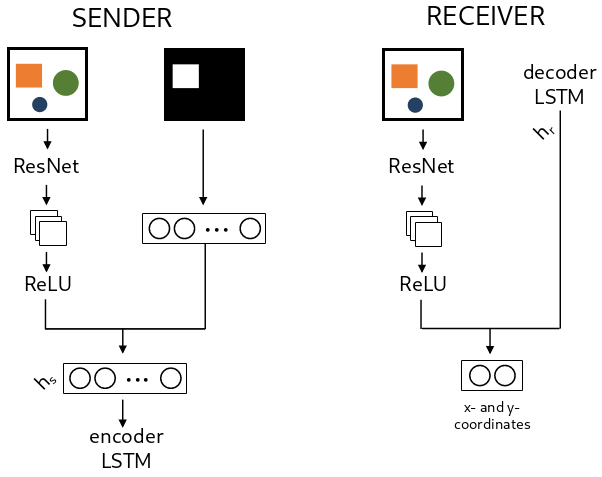
\includegraphics[width=.7\linewidth]{figures/arch_coordinate_predictor_game.png}
    \caption{Simplified architecture of the masked coordinate predictor game}
    \label{fig:coordinate_predictor_game_architecture}
    % SD: Again, why LSTM, are we inceremtally identifying the image while we are processing each input word?
    % DK: because it's a message sequence of discrete symbols (done)
\end{figure}

For the second approach, the masked image is passed only through a feature extractor.
Both the resulting encoding of the masked image and the encoding of the original image are each passed through separate linear layer to adjust their dimensions to the same embedding size $e_s$.
These embeddings are subsequently concatenated and reduced to the hidden size $h_s$ with a final linear layer.

The receiver contains of two parts.
First, the original image is encoded with an image encode of the same setup.
This encoded image is flattened and concatenated with the final hidden state of the wrapper LSTM encoding the message received by the receiver.
The resulting vector is the passed through the second part of the receiver, the predictor.
This predictor contains of three linear layers, reducing the dimensions to 1024, 1024 and 2 respectively.
A \emph{ReLU} function is applied in between.
This setup is trained to combine the important information from both the image and the message of the sender.
The euclidean distance between the resulting prediction of the center point and the true center of the target object is calculated and the weights of both agents are adapted accordingly.

As in the pre-experiments, the agents are trained first the 'CLEVR single' dataset to understand if they are capable of predicting locations in an image together.
In a next step, the 'Dale-2' and 'Dale-5' datasets are used to test if the agents are able to first communicate a target object and second describe the target object discriminatively with a small vocabulary.

During the experiments, the effects of the following variables are compared:
(1) the vocabulary size $|V|$,
(2) the LSTM hidden size of the sender wrapper $h_s$,
(3) the LSTM hidden size of the receiver wrapper $h_r$ and
(4) the embedding size of the sender $e_s$.
As before, the metrics to evaluate the results are the same as in the pre-experiments.

\subsection*{Results}
In the final setup, the agents are tasked with communicating objects with fewer infused human knowledge.
Table \ref{tab:results_dale_predictor_game} shows the results for the setup, in which the sender is pointed towards the target object with a human description based on the GRE algorithm.
Hereby, the 'CLEVR single' dataset acts as a baseline, to test if the agents are able to predict coordinates of objects at all.
In every configuration of the variables, the agents achieve a very high performance.
The worst average distance across the test dataset is 10 pixels, which still points onto an object.
Also the accuracy, which evaluates how many guesses of the receiver were pointing onto an object reflects this fact.
All configuration achieve an accuracy higher than 96,7\%.
% SD: Just occured to me: how do we measure accuracy if we are predicting numbers (numeric prediction)?
% DK: same as in the experiments with one model (done)
This aligns also with the results from the single neural models, where the average distance was similarly low.
In general, this shows that the agents are able to predict coordinates together.
However, the question arises if the message by the sender has actually an effect on the receivers' decision, or if the receiver learns to point towards the target coordinates on his own and the message is ignored.
Having a look at the transferred messages, it in fact shows that the receiver learns to point towards the target object on its own.
% SD: But how could it do so if the visual data is randomly distribution. It must rely on the message as that is the only source of information.
% DK: it does it in the same way as the single model above (TODO)
As in the experiment before, all communicated messages contain the same symbol independent of the input image.

\begin{table}[h]
    \centering
    \begin{tabular}{ccc|ccc|ccc|ccc}
        \toprule
              &         &         & \multicolumn{3}{c}{\textbf{CLEVR single}} & \multicolumn{3}{c}{\textbf{Dale-2}} & \multicolumn{3}{c}{\textbf{Dale-5}}                                                                                                       \\\cmidrule(lr){4-6}\cmidrule(lr){7-9}\cmidrule(lr){10-12}
        $|V|$ & $h_{s}$ & $h_{r}$ & \textbf{Dist.}                            & \textbf{Acc.}                       & \textbf{length}                     & \textbf{Dist.} & \textbf{Acc.} & \textbf{length} & \textbf{Dist.} & \textbf{Acc.} & \textbf{length} \\\midrule
        {10}  & {10}    & {10}    & {10,1}                                    & {98,5\%}                            & {1}                                 & {36,5}         & {19,9\%}      & {1}             & {45,7}         & {14,4\%}      & {1}             \\
        {13}  & {10}    & {10}    & {6}                                       & {99\%}                              & {0}                                 & {38}           & {20,4\%}      & {1}             & {47,3}         & {10,8\%}      & {1}             \\
        {20}  & {10}    & {10}    & {9,7}                                     & {96,7\%}                            & {1}                                 & {37,3}         & {21,2\%}      & {1}             & {47,3}         & {11,3\%}      & {0}             \\
        {100} & {10}    & {10}    & {7,7}                                     & {98,4\%}                            & {1}                                 & {40,4}         & {21,7\%}      & {1}             & {45,4}         & {10,8\%}      & {1}             \\
        {100} & {100}   & {100}   & {7,5}                                     & {96,9\%}                            & {1}                                 & {40,1}         & {17,8\%}      & {1}             & {44,3}         & {11,8\%}      & {0}             \\
        \bottomrule
    \end{tabular}
    \caption{Results of the description coordinate predictor: $|V|$ are different vocabulary sizes and $h$ hidden sizes.}
    \label{tab:results_dale_predictor_game}
\end{table}

When the experiments are run on the 'Dale-2' dataset, the results are much worse.
For the \emph{description coordinate predictor}, the average distance ranges from 36,5 pixels to 40,4 pixels.
The configuration with a vocabulary size of only 10 symbols fares the best, while a vocabulary of 100 symbols produces the worst results.
% SD: Remind the reader what is the size of the image so that they can interprert the distance relatively to that.
% DK: TODO
Still, the accuracy shows that around 19,9\% to 21,7\% of the guesses are on the target object.
Here, the configurations with higher vocabulary sizes fare slightly better, but the differences are very small and likely due to other factors.

The results for 'Dale-5' dataset are even worse, but are comparable with the results with a single neural model.
Apparently, the agents are not able to communicate the target object, and the predictions by the receiver are general in the middle of the image, which results in an average distance of around 45 to 50 pixels.
The differences of the mean distances are not very significant in this range, to allow an analysis of the different configurations.
% SD: I don't understand this
% DK: TODO

\begin{table}[h]
    \centering
    \begin{tabular}{cccc|ccc|ccc|ccc}
        \toprule
              &         &         &         & \multicolumn{3}{c}{\textbf{CLEVR single}} & \multicolumn{3}{c}{\textbf{Dale-2}} & \multicolumn{3}{c}{\textbf{Dale-5}}                                                                                                       \\\cmidrule(lr){5-7}\cmidrule(lr){8-10}\cmidrule(lr){11-13}
        $|V|$ & $h_{s}$ & $h_{r}$ & $e_{s}$ & \textbf{Dist.}                            & \textbf{Acc.}                       & \textbf{length}                     & \textbf{Dist.} & \textbf{Acc.} & \textbf{length} & \textbf{Dist.} & \textbf{Acc.} & \textbf{length} \\\midrule
        {10}  & {10}    & {10}    & {1024}  & {10,8}                                    & {93,1\%}                            & {1}                                 & {34,8}         & {24,3\%}      & {0}             & {44,3}         & {11,8\%}      & {1}             \\
        {10}  & {10}    & {10}    & {512}   & {9,3}                                     & {92\%}                              & {1}                                 & {36,3}         & {19,9\%}      & {0,7}           & {45,9}         & {12,7\%}      & {1}             \\
        {13}  & {10}    & {10}    & {1024}  & {7,8}                                     & {96,8\%}                            & {1}                                 & {36,3}         & {20,2\%}      & {0}             & {45,4}         & {11,4\%}      & {1}             \\
        {20}  & {10}    & {10}    & {1024}  & {6,6}                                     & {98,3\%}                            & {1}                                 & {37,8}         & {16,1\%}      & {1}             & {45,2}         & {11\%}        & {1}             \\
        {100} & {10}    & {10}    & {1024}  & {5,2}                                     & {98,5\%}                            & {1}                                 & {37,4}         & {20,1\%}      & {1}             & {43,6}         & {16,7\%}      & {1}             \\
        {100} & {100}   & {100}   & {1024}  & {12,5}                                    & {92,1\%}                            & {1}                                 & {36,5}         & {20,7\%}      & {1}             & {44,6}         & {12,7\%}      & {1}             \\
        \bottomrule
    \end{tabular}
    \caption{Results of the masked coordinate predictor: $|V|$ are different vocabulary sizes, $h$ hidden sizes and $e$ embedding sizes.}
    \label{tab:results_masked_predictor_game}
\end{table}

Finally looking at the setup, when using the masked image as an input shows that the results are similarly bad as when using the encoded captions.
This is easily explainable with the emerged language.
For both the experiments using the encoded captions and the experiments using masked images as input, no meaningful symbols are transferred.
% SD: A bit gloomy result. Negative result is okay but then we need an explanation why this is so and have some ideas what to change. What we can learn from these results?
% DK: TODO
Following, the receiver needs to solve the task alone and the different setups of the sender don't play any role in the overall success.
% SD: This identifies that the problem lies in how the sender encodes the messages; what is its policy to generate longer strings or reuse the word. Without a policy the sender will never be motivated to encode longer messages and therefore rely on single-word expressions.
% SD: The second problem is the size of these networks. We should also test smaller embedding sizes than 10. Practice shows that the embedding sizes can be even several magnitues smaller than the vocabulary sizes, cf. the Bengio paper and word2vec.
% SD: The reason why the system is not performing well on the pointing task is that it does not have the right features to learn from. It ahs visual information WHAT these objects are (what do they look like) but they do not have information WHERE these objects are,. John Kelleher and I wrote an opiiuon piece about the lack of spatial knowledge required to model spatial descriptions in CNNs. The same problem is probably occuring here. Replacing the features or adding geometric features that would communicate geometric relations that allow pointing would improve the task and also we would expect that a vocabulary would emerge such that some words are more biased towards visual features (to identify objects) and some more to geometric features (to locate them), hence WHAT and WHERE.
% SD: J. D. Kelleher and S. Dobnik. What is not where: the challenge of integrating spatial representations into deep learning architectures. In S. Dobnik and S. Lappin, editors, Proceedings of the Conference on Logic and Machine Learning in Natural Language (LaML 2017), Gothenburg, 12 –13 June, volume 1 of CLASP Papers in Computational Linguistics, pages 41–52, Gothenburg, Sweden, November 2017. Department of Philosophy, Linguistics and Theory of Science (FLOV), University of Gothenburg, CLASP, Centre for Language and Studies in Probability.https://gup.ub.gu.se/publication/262970?lang=en
% SD: Overall, the thesis has a lot of potential if we could implement all this
% DK: TODO

When comparing these results to the neural models in Section \ref{sec:reference_resolution} that are not part of a language game, it can be seen that the metrics are very similar for all datasets.
The model was already not able to solve the task without the increased complexity of a language game.
This therefore indicates that the challenge for the agents doesn't lie in grounding the extracted features in new symbols, but already in extracting the features in the first place.
\newpage

\section{Analysis of the emerged languages}
\label{sec:analysis_language}
The languages that emerge are analyzed in two ways.
First, for each language that emerges through successful communication, a score is calculated that represents the similarity of the messages to valid English referring expressions.
In a second step, several languages are analyzed qualitatively, to determine what certain symbols mean and what they might refer to in the visual scenes.
\cmtDK[inline]{talks about why and which few languages}
\cmtDK[inline]{chosen salience order might be due to number of possibilities (more efficient to exclude larger number of distractors instantly)}

To compare the emerged language to English in a \textbf{quantitative} way, a probing approach is used.
Probing can be used to analyze and interpret the hidden representations in neural networks.
Hereby, a second neural model is trained to predict selected linguistic properties on the basis of the hidden representations.
If this model is successfully able to predict the linguistic properties, the hidden representations are connected to them.
If second model can't be trained, it indicates that there is no correlation between the hidden representation and the linguistic property.
In the case of the emerged language, a neural model is trained to translate the messages of the sender into English referring expressions, based on the GRE algorithm by \citet{Dale1995}.
Recall, that this incremental is based on an order in salience for the attributes.
In English, \citet{Dale1995} propose the order of \emph{shape} > \emph{color} > \emph{size}.
However, there is no policy for the agents, that enforces specifically this order or indeed any salience order.
For this reason, the emerged languages are compared to all possible salience orders, given the three attributes \emph{shape}, \emph{color} and \emph{size}.
This will show if first, the languages follow any salience order and secondly, which attributes are more important for the agents to communicate.
% SD: The probing test is to show how well the emerged language can be trasnlated into English descriptions consistting of labels of scene features using Dale and Reiter idea of incrementality. However, we would need to know now what was the policy of the sender to generate message. Was this similar to Dale and Reiter to enforce longer descriptions?
% DK: done

The probing model consists of an encoder LSTM, one linear layer and a decoder LSTM.
The encoder LSTM encodes the messages of the emerged language.
Its final hidden state is used as a representation of the meaning of the complete message and passed through the linear layer, which learns an abstract representation of the message.
The dimension of the linear layer is kept small to prevent memorizing the dataset and force the model to find abstract connections between the input and the target.
The resulting vector is used as the initial state of the decoder LSTM.
The decoder LSTM is then trained to produce the English referring expression.
Both LSTMs have an embedding dimension of $LSTM_e=10$ and a hidden size of $LSTM_{out}=10$, while the linear layer has a size of $l=10$.
During decoding, teacher forcing is applied.
The success of the model is validated calculating cross entropy between the models predictions and the target English referring expression.
Since generalization doesn't play a role for probing, no dropout is applied and the model is trained and validated on the complete dataset; no test or validation split is used.
The models are trained for 200 epochs with a learning rate of $lr=0,004$ and a batch size of 32 samples per batch.

The translation model will learn two characteristics with this setup.
First, it can learn to find correlations between the emerged language and the English referring expressions, which is the goal of the probing.
But secondly, it can also learn underlying patterns in the English referring expressions that are independent of the emerged language.
For instance, it can learn that the referring expressions are likely to be two symbols long, or that for instance 'cube' is the most common shape.
This second characteristic will lead to a low loss during training, even though there are no connections to the emerged language.
In this test, only the first characteristic is interesting and would show the correlation between the emerged language and English referring expressions.
For that reason, two reference baselines are calculated for each salience order of the attributes, to eliminate the influence of the second characteristic.
% SD: Baselines?
% DK: (done)
The first baseline $L_{baseline}$ uses a non-informative input for the encoder LSTM, more specifically it always receives a vector of zeros and therefore can't learn any meaningful representation in the linear layer; the input for the decoder LSTM is the same for every sample.
By this, the model is trained to learn the structural patterns in the English referring expressions.
The resulting loss is the highest possible loss the model can achieve, independent of the input.
Resulting, if the emergent language is connected to English, the loss will be lower than this baseline.
If not, the loss will be as high as this baseline.
On the other side, the lowest possible loss $L_{English}$ is calculated, by using the English referring expressions as both input and target.
This verifies that the model is able to learn an abstract representation from the input and the resulting loss should be close to zero (since the input is perfectly correlated to the target).
These two references are used, to normalize the results of the actual emergent languages $L_{em}$, using the formula $L_{norm} = \frac{L_{em}-L_{English}}{L_{baseline} - L_{English}}$.
A loss close to $L_{baseline}$ will lead to 100\%, while a loss as $L_{English}$ will lead to 0\%.
% SD: Is this encessary? But when and where is this loss using 0 inouts calculated?
% DK: TODO, QUESTION
By doing this, all configurations can be compared directly to each other.
The lower $L_{norm}$, the higher the correlation between the emerged language and English referring expressions.

Tables \ref{tab:probing:discriminator:dale-2} to \ref{tab:probing:attention-predictor:colour} show the normalized losses $L_{norm}$ of the probing for the different tasks on all three datasets.
Hereby, only languages are listed for experiments in which the agents communicated successfully, that is $L_{norm}$ is lower than 100\%.
The first thing that can be noticed is that across almost all languages emerged through successful communication, $L_{norm}$ is lower than 100\% with at least one salience order, which shows that they make use of the attributes in some way.
On the other side, no language reaches an $L_{norm}$ close to 0, that is no language correlates perfectly with English referring expressions.
The closest is a language with $L_{norm}$ just above 40\%.
This shows that while many emerged languages have similarities with English, they make use of either other additional visual characteristics in the scenes or use different linguistic structures.

In the following paragraphs, languages will be referred to by their message length $n$ and their vocabulary size $|V|$ as $Lang_{n,|V|}$.

\begin{table}[ht]
    \centering
    \begin{tabular}{cc|c|c|c|c|c|c}
        \toprule
        $n$ & $|V|$ & \textbf{C > Sh > Si}              & \textbf{C > Si > Sh}              & \textbf{Sh > C > Si}     & \textbf{Sh > Si > C}     & \textbf{Si > C > Sh}     & \textbf{Si > Sh > C}     \\\midrule
        {1} & {2}   & \textcolor{red}{95,5\%}           & \textcolor{red}{97,57\%}          & {86,98\%}                & {81,43\%}                & \textcolor{red}{91,67\%} & {86,45\%}                \\
        {1} & {10}  & \textcolor{red}{96,11\%}          & \textcolor{red}{96,9\%}           & {89,61\%}                & {85\%}                   & {89,4\%}                 & {84,49\%}                \\
        {1} & {16}  & \textcolor{red}{95,19\%}          & \textcolor{red}{96,56\%}          & {87,25\%}                & {81,22\%}                & {89,34\%}                & {83,13\%}                \\
        {1} & {50}  & \textcolor{red}{96,61\%}          & \textcolor{red}{97,07\%}          & \textcolor{red}{91,26\%} & {85,75\%}                & {87,14\%}                & {82,61\%}                \\
        {1} & {100} & \textcolor{red}{95,91\%}          & \textcolor{red}{96,73\%}          & \textcolor{red}{90,63\%} & {86,01\%}                & {88,95\%}                & {84,17\%}                \\
        {2} & {2}   & \textcolor{red}{99,67\%}          & \textcolor{red}{99,91\%}          & \textcolor{red}{97,02\%} & \textcolor{red}{95,37\%} & \textcolor{red}{96,97\%} & \textcolor{red}{94,64\%} \\
        {2} & {10}  & \textcolor{red}{96,36\%}          & \textcolor{red}{96,34\%}          & \textcolor{red}{91,32\%} & {86,75\%}                & {87,69\%}                & {82,87\%}                \\
        {2} & {16}  & \textcolor{red}{95,63\%}          & \textcolor{red}{97,12\%}          & {88,11\%}                & {83,21\%}                & {89,86\%}                & {85,35\%}                \\
        {2} & {50}  & \textcolor{red}{95,34\%}          & \textcolor{red}{97,3\%}           & {85,48\%}                & {80,89\%}                & \textcolor{red}{92,22\%} & {86,18\%}                \\
        {2} & {100} & \textcolor{red}{94,88\%}          & \textcolor{red}{96,32\%}          & {87,37\%}                & {81,17\%}                & {88,35\%}                & {82,61\%}                \\
        {3} & {2}   & \textcolor{red}{\textbf{94,03\%}} & \textcolor{red}{96,96\%}          & \textbf{79,59\%}         & \textbf{74,54\%}         & \textcolor{red}{92,32\%} & {85,63\%}                \\
        {3} & {10}  & \textcolor{red}{96,1\%}           & \textcolor{red}{95,97\%}          & \textcolor{red}{90,45\%} & {84,84\%}                & {85,98\%}                & {80,5\%}                 \\
        {3} & {16}  & \textcolor{red}{95,71\%}          & \textcolor{red}{\textbf{95,1\%}}  & \textcolor{red}{90,97\%} & {85,33\%}                & {81\%}                   & \textbf{75,56\%}         \\
        {3} & {50}  & \textcolor{red}{96,32\%}          & \textcolor{red}{\textbf{94,55\%}} & \textcolor{red}{92,5\%}  & {86,81\%}                & \textbf{80,48\%}         & {75,73\%}                \\
        {3} & {100} & \textcolor{red}{95,33\%}          & \textcolor{red}{97,82\%}          & {86,05\%}                & {81,33\%}                & \textcolor{red}{93,91\%} & {88,54\%}                \\
        {4} & {2}   & \textcolor{red}{96,81\%}          & \textcolor{red}{95,12\%}          & \textcolor{red}{93,03\%} & {87,41\%}                & \textbf{80,73\%}         & \textbf{75,47\%}         \\
        {4} & {10}  & \textcolor{red}{95,31\%}          & \textcolor{red}{97,26\%}          & {86,9\%}                 & {82,67\%}                & \textcolor{red}{92,39\%} & {86,98\%}                \\
        {4} & {16}  & \textcolor{red}{95,63\%}          & \textcolor{red}{\textbf{94,65\%}} & \textcolor{red}{91,99\%} & {86,65\%}                & \textbf{79,23\%}         & \textbf{74,54\%}         \\
        {4} & {50}  & \textcolor{red}{94,76\%}          & \textcolor{red}{96,69\%}          & {86,8\%}                 & {81,33\%}                & {89,65\%}                & {83,92\%}                \\
        {4} & {100} & \textcolor{red}{96,16\%}          & \textcolor{red}{97,94\%}          & {89,57\%}                & {85,18\%}                & \textcolor{red}{92,56\%} & {87,74\%}                \\
        {6} & {2}   & \textcolor{red}{95,73\%}          & \textcolor{red}{96,99\%}          & {87,77\%}                & {83,27\%}                & \textcolor{red}{91,77\%} & {86,34\%}                \\
        {6} & {10}  & \textcolor{red}{\textbf{94,59\%}} & \textcolor{red}{99,89\%}          & {86,24\%}                & {81,46\%}                & \textcolor{red}{91,42\%} & {86,43\%}                \\
        {6} & {16}  & \textcolor{red}{95,51\%}          & \textcolor{red}{96,3\%}           & {88,89\%}                & {83,24\%}                & {87,61\%}                & {82,71\%}                \\
        {6} & {50}  & \textcolor{red}{\textbf{94,66\%}} & \textcolor{red}{97,43\%}          & \textbf{84,93\%}         & \textbf{78,61\%}         & \textcolor{red}{91,48\%} & {83,66\%}                \\
        {6} & {100} & \textcolor{red}{95,37\%}          & \textcolor{red}{97,77\%}          & \textbf{83,75\%}         & \textbf{80,84\%}         & \textcolor{red}{93,96\%} & {89,02\%}                \\
        \bottomrule
    \end{tabular}
    \caption{Normalized losses $L_{norm}$ of the probing model on emerged languages of the \emph{discrimination games} on the 'Dale-2' dataset. The emerged languages are probed with different salience orders where 'C' corresponds to the \emph{color}, 'Sh' to the \emph{shape} and 'Si' to the \emph{size}. The table only includes languages, with which the agents could successfully solve the task.}
    \label{tab:probing:discriminator:dale-2}
\end{table}

Looking at the results for the discriminator, one can see that the results are very different for each dataset.
On the 'Dale-2' dataset $L_{norm}$ is relatively high for all salience orders (see Table \ref{tab:probing:discriminator:dale-2}).
Yet, the correlation to English referring expressions with the \emph{color} as most important attribute is the lowest.
When the \emph{color} attribute is in the second position, the correlation becomes higher, but the highest correlation is achieved when the \emph{color} has the least importance.
This shows that the agents don't use the \emph{color} in the communication, but rather rely on \emph{shape} and \emph{size}.
The order of importance of these attributes however is not as clear.
For some combinations of the message length $n$ and vocabulary size $|V|$, the \emph{size} seems to be the dominant attribute, while for others the \emph{shape} seems more important in the communication.
Interestingly, one can see that for many languages only one salience order has a low $L_{norm}$, while the $L_{norm}$ for the remaining salience orders with a different attribute in the first position is higher.
This applies for example to $Lang_{3,2}$, where the loss for 'Sh > Si > C' is 74,54\% while the second lowest is only at 85,63\% for 'Si > Sh > C'.
The same can be seen for instance for $Lang_{3,16}$ in the other direction.
This difference indicates that the agents are relying mostly on the most important attribute of this salience order to discriminate the target object.
If the $L_{norm}$ for instance were similar for the salience orders 'Sh > Si > C' and 'Si > Sh > C', this would mean that the emerged language could be connected to both salience orders in the same way.
Following, the agents would use the \emph{shape} as often as \emph{size} to discriminate the objects.
This is however only the case on the 'Dale-2' dataset when the loss is higher (for instance languages $Lang_{2,16}$, $Lang_{2,100}$ or $Lang_{6,16}$).
Since the lowest $L_{norm}$ with 74,54\% is still very high compared to a complete correlation (0\%), the agents seem to encode additionally other information in their messages.

Looking at the influence of $n$ and $|V|$, one can see that across almost all values, there is at least some correlation to one salience order.
The correlation seems to be highest with $n \in \{3,4\}$, where the loss can reach down 74,54\%.
Hereby, the most important attribute in the messages seems to be the \emph{size}.
For the remaining message lengths $n$, the loss stays mostly between 80\% and 85\%.
For $n \in \{2,6\}$ the \emph{shape} seems to be the most dominant attribute, while for $n=1$ the \emph{size} and \emph{shape} seem to have a similar importance.
The influence of the vocabulary size $|V|$ is not as clear.
Small to medium-sized vocabularies seem to promote higher correlations with English referring expressions, but also languages with $|V|=100$ can reach losses of around 80\%.

\begin{table}[ht]
    \centering
    \begin{tabular}{cc|c|c|c|c|c|c}
        \toprule
        $n$ & $|V|$ & \textbf{C > Sh > Si}     & \textbf{C > Si > Sh}     & \textbf{Sh > C > Si}     & \textbf{Sh > Si > C}     & \textbf{Si > C > Sh} & \textbf{Si > Sh > C} \\\midrule
        {1} & {2}   & \textcolor{red}{94,96\%} & \textcolor{red}{91,27\%} & \textcolor{red}{94,51\%} & \textcolor{red}{90,99\%} & {88,52\%}            & {88,17\%}            \\
        {1} & {10}  & {84,34\%}                & {84,03\%}                & {80,91\%}                & {73,23\%}                & {79,95\%}            & {72,34\%}            \\
        {1} & {16}  & {86,27\%}                & {84,96\%}                & {82,76\%}                & {75,35\%}                & {80,72\%}            & {74,04\%}            \\
        {1} & {50}  & {85,95\%}                & {84,4\%}                 & {82,96\%}                & {74,97\%}                & {80,2\%}             & {73,54\%}            \\
        {1} & {100} & {86,31\%}                & {85,58\%}                & {82,9\%}                 & {76,03\%}                & {81,64\%}            & {74,62\%}            \\
        {2} & {10}  & \textbf{82,66\%}         & {83,23\%}                & \textbf{78,51\%}         & {71,01\%}                & {78,89\%}            & {70,61\%}            \\
        {2} & {16}  & {89,78\%}                & {85,53\%}                & {87,68\%}                & {80,64\%}                & {81,06\%}            & {77,24\%}            \\
        {2} & {50}  & {84,4\%}                 & {82,65\%}                & {80,62\%}                & {71,42\%}                & {77,53\%}            & {69,46\%}            \\
        {2} & {100} & {89,65\%}                & {85,3\%}                 & {87,26\%}                & {79,91\%}                & {80,88\%}            & {77,1\%}             \\
        {3} & {2}   & {87,19\%}                & {86,93\%}                & {83,99\%}                & {78,18\%}                & {83,65\%}            & {77,08\%}            \\
        {3} & {10}  & {87,15\%}                & {84,67\%}                & {84,01\%}                & {76,24\%}                & {80,41\%}            & {74,11\%}            \\
        {3} & {50}  & \textbf{82,98\%}         & {82,25\%}                & {78,85\%}                & {70,62\%}                & {77,42\%}            & {69,27\%}            \\
        {3} & {100} & {83,78\%}                & {83,07\%}                & {80,23\%}                & {72,15\%}                & {78,94\%}            & {71,1\%}             \\
        {4} & {2}   & {89,23\%}                & {87,43\%}                & {87,09\%}                & {81,45\%}                & {83,83\%}            & {79,11\%}            \\
        {4} & {10}  & {88,66\%}                & {84,83\%}                & {85,9\%}                 & {78,98\%}                & {80,2\%}             & {75,64\%}            \\
        {4} & {16}  & {83,14\%}                & \textbf{81,51\%}         & \textbf{78,15\%}         & \textbf{70,21\%}         & \textbf{77,32\%}     & \textbf{68,48\%}     \\
        {4} & {50}  & {87,62\%}                & {84,38\%}                & {85,25\%}                & {77,29\%}                & {79,94\%}            & {74,03\%}            \\
        {4} & {100} & \textcolor{red}{90,17\%} & {85,76\%}                & {87,68\%}                & {80,71\%}                & {81,37\%}            & {78,1\%}             \\
        {6} & {10}  & \textbf{82,03\%}         & \textbf{80,51\%}         & \textbf{77,46\%}         & \textbf{68,63\%}         & \textbf{75,71\%}     & \textbf{67,15\%}     \\
        {6} & {16}  & {84,73\%}                & \textbf{81,12\%}         & {80,99\%}                & \textbf{70,5\%}          & \textbf{76,06\%}     & \textbf{69,12\%}     \\
        {6} & {50}  & {86,95\%}                & {85,13\%}                & {84,06\%}                & {76,95\%}                & {80,11\%}            & {74,51\%}            \\
        {6} & {100} & {86,15\%}                & {82,19\%}                & {83,56\%}                & {75,56\%}                & {77,76\%}            & {72,47\%}            \\
        \bottomrule
    \end{tabular}
    \caption{Normalized losses $L_{norm}$ of the probing model on emerged languages of the \emph{discrimination games} on the 'Dale-5' dataset. The emerged languages are probed with different salience orders where 'C' corresponds to the \emph{color}, 'Sh' to the \emph{shape} and 'Si' to the \emph{size}. The table only includes languages, with which the agents could successfully solve the task.}
    \label{tab:probing:discriminator:dale-5}
\end{table}

The emerged languages on the 'Dale-5' dataset have generally a higher correlation to English referring expressions (see Table \ref{tab:probing:discriminator:dale-5}).
For almost all salience orders and emerged languages, the loss is lower than 90\%.
In the best cases, it even reaches down to 67,15\%.
Again, the \emph{size} and the \emph{shape} are mostly communicated between the agents, but the \emph{color} now plays a bigger role in the messages.
The agents seem to need to rely on more attributes to discriminate the target object.
This aligns also with English referring expressions, where the average length of the referring expressions across the whole 'Dale-5' dataset is longer than for the 'Dale-2' dataset.
However, opposed to the 'Dale-2' dataset, there are almost no languages, where there is one dominant attribute.
More often the loss is similar for two salience orders with different primary attributes.
For instance the salience orders 'Sh > Si > C' and 'Si > Sh > C' both provide losses around 70\% for $Lang_{6,16}$.
Only the languages $Lang_{2,16}$, $Lang_{4,10}$, $Lang_{4,50}$ and $Lang_{6,100}$ have differences of more than 3\% points for these salience orders.
This indicates, that the agents make use of both \emph{shape} and \emph{size} similarly often, while the \emph{color} is used for much fewer images.

When the agents are able to produce longer messages, their languages seem to have more similarities with possible English languages.
With $n>1$ the agents produce languages that can have losses lower than 70\% for the salience order 'Si > Sh > C'.
Yet, languages with $n=1$ are not far off and have mostly losses between 72\% and 75\%.
Looking at the vocabulary size, languages with $|V|=2$ are less likely to emerge and if they emerge they have a lower correlation with English.
The best results are produces with $|V| \in \{10,16\}$ for longer messages (for instance $Lang_{4,16}$, $Lang_{6,10}$ and $Lang_{6,16}$), while shorter messages fare generally better with a larger vocabulary of $|V| \in \{50,100\}$ ($Lang_{2,50}$, $Lang_{3,50}$ and $Lang_{3,100}$).

\begin{table}[ht]
    \centering
    \begin{tabular}{cc|c|c|c|c|c|c}
        \toprule
        $n$ & $|V|$ & \textbf{C > Sh > Si}     & \textbf{C > Si > Sh}     & \textbf{Sh > C > Si}     & \textbf{Sh > Si > C}     & \textbf{Si > C > Sh}     & \textbf{Si > Sh > C}     \\\midrule
        {1} & {2}   & \textcolor{red}{91,62\%} & \textcolor{red}{91,57\%} & \textcolor{red}{94,31\%} & \textcolor{red}{95,13\%} & \textcolor{red}{93,11\%} & \textcolor{red}{94,92\%} \\
        {1} & {10}  & {79,08\%}                & {79,08\%}                & {85,04\%}                & {86,86\%}                & {82,37\%}                & {86,38\%}                \\
        {1} & {16}  & {84,02\%}                & {83,96\%}                & {88,67\%}                & {89,65\%}                & {86,36\%}                & {89,36\%}                \\
        {1} & {50}  & \textcolor{red}{93,88\%} & \textcolor{red}{93,74\%} & \textcolor{red}{95,03\%} & \textcolor{red}{95,49\%} & \textcolor{red}{94,64\%} & \textcolor{red}{95,35\%} \\
        {2} & {10}  & {88,67\%}                & {88,36\%}                & {89,59\%}                & \textcolor{red}{90,77\%} & \textcolor{red}{90,01\%} & {89,81\%}                \\
        {2} & {16}  & {81,13\%}                & {81,02\%}                & {86,16\%}                & {87,97\%}                & {83,85\%}                & {87,56\%}                \\
        {3} & {2}   & {83,38\%}                & {83,46\%}                & {88,21\%}                & {89,71\%}                & {86,05\%}                & {89,37\%}                \\
        {3} & {10}  & \textbf{77\%}            & \textbf{76,77\%}         & \textbf{83,54\%}         & \textbf{85,57\%}         & \textbf{79,97\%}         & \textbf{84,9\%}          \\
        {3} & {16}  & \textcolor{red}{93,52\%} & \textcolor{red}{93,6\%}  & \textcolor{red}{94,16\%} & \textcolor{red}{94,14\%} & \textcolor{red}{93,75\%} & \textcolor{red}{93,55\%} \\
        {4} & {10}  & \textbf{68,04\%}         & \textbf{66,51\%}         & \textbf{76,33\%}         & \textbf{78,56\%}         & \textbf{71,42\%}         & \textbf{78,56\%}         \\
        {4} & {16}  & \textbf{75,1\%}          & \textbf{74,93\%}         & \textbf{81,2\%}          & \textbf{83,35\%}         & \textbf{77,6\%}          & \textbf{82,76\%}         \\
        {6} & {2}   & {84,21\%}                & {84,02\%}                & {88,41\%}                & {89,77\%}                & {86,61\%}                & {89,35\%}                \\
        \bottomrule
    \end{tabular}
    \caption{Normalized losses $L_{norm}$ of the probing model on emerged languages of the \emph{discrimination games} on the 'CLEVR color' dataset. The emerged languages are probed with different salience orders where 'C' corresponds to the \emph{color}, 'Sh' to the \emph{shape} and 'Si' to the \emph{size}. The table only includes languages, with which the agents could successfully solve the task.}
    \label{tab:probing:discriminator:colour}
\end{table}

Finally on the 'CLEVR color' dataset, much fewer languages emerge (see Table \ref{tab:probing:discriminator:colour}).
Those languages that emerge have very different levels of correlation to English
While three languages stay above 90\% for all salience orders, most of them stay between 80\% and 90\%.
Four languages even get below 80\% for the salience orders where the \emph{color} is the most important attribute.
One of those even reaches 66,51\%, the highest correlation across all emerged languages on the discrimination task.
Unsurprisingly, the \emph{color} is now the most important attribute.
The loss with the remaining salience orders is still relatively low, but this is likely due to the fact, that the color occurs in any referring expression as it is the only discriminating attribute.
The probing model can therefore easily connect this pattern to the emerged language.
As expected, the losses for 'Sh > Si > C' and 'Si > Sh > C' are almost the same, which indicates that the agents make (no) use of both \emph{shape} and \emph{size} in the same way.

Even though only one attribute would need to be communicated, languages with $n \in \{3,4\}$ tend to be closer to English referring expressions.
Hereby, vocabulary sizes of $|V| \in \{10,16\}$ produce the most correlating languages, while languages with only 2 symbols have relatively high losses.
The agents were not able to communicate with vocabulary sizes larger than 16.


\begin{table}[ht]
    \centering
    \begin{tabular}{cc|c|c|c|c|c|c}
        \toprule
        $n$ & $|V|$ & \textbf{C > Sh > Si}     & \textbf{C > Si > Sh}              & \textbf{Sh > C > Si}     & \textbf{Sh > Si > C}     & \textbf{Si > C > Sh}     & \textbf{Si > Sh > C}     \\\midrule
        {1} & {2}   & \textcolor{red}{95,07\%} & \textcolor{red}{98,06\%}          & {86,63\%}                & {85,3\%}                 & \textcolor{red}{96,26\%} & \textcolor{red}{93,32\%} \\
        {1} & {10}  & \textcolor{red}{90,8\%}  & \textcolor{red}{96,4\%}           & {71,88\%}                & {69,29\%}                & \textcolor{red}{94,05\%} & {85,13\%}                \\
        {1} & {16}  & \textcolor{red}{91,47\%} & \textcolor{red}{96,96\%}          & {71,2\%}                 & {66,82\%}                & \textcolor{red}{93,83\%} & {83,35\%}                \\
        {1} & {50}  & \textcolor{red}{93,26\%} & \textcolor{red}{96,63\%}          & {77,53\%}                & {71,94\%}                & \textcolor{red}{93,56\%} & {84,62\%}                \\
        {1} & {100} & \textcolor{red}{93,5\%}  & \textcolor{red}{97,86\%}          & {77,42\%}                & {71,93\%}                & \textcolor{red}{94,68\%} & {85,77\%}                \\
        {2} & {2}   & \textcolor{red}{93,57\%} & \textcolor{red}{97,72\%}          & {80,89\%}                & {79,8\%}                 & \textcolor{red}{96,08\%} & \textcolor{red}{90,71\%} \\
        {2} & {10}  & \textbf{84,86\%}         & \textcolor{red}{\textbf{92,07\%}} & {58,8\%}                 & \textbf{52,09\%}         & \textbf{88,36\%}         & {77,01\%}                \\
        {2} & {16}  & {87,29\%}                & \textcolor{red}{92,88\%}          & {68,52\%}                & {71,5\%}                 & \textcolor{red}{92,56\%} & {83,9\%}                 \\
        {2} & {50}  & {89,15\%}                & \textcolor{red}{95\%}             & {68,19\%}                & {68,93\%}                & \textcolor{red}{93,11\%} & {83,95\%}                \\
        {2} & {100} & \textcolor{red}{91,06\%} & \textcolor{red}{96,14\%}          & {71,98\%}                & {67,23\%}                & \textcolor{red}{92,81\%} & {82,71\%}                \\
        {3} & {2}   & \textcolor{red}{93,05\%} & \textcolor{red}{97,15\%}          & {82,41\%}                & {77,36\%}                & \textcolor{red}{94,43\%} & {88,8\%}                 \\
        {3} & {10}  & {88,52\%}                & \textcolor{red}{95,41\%}          & {66,61\%}                & {63,63\%}                & \textcolor{red}{92,25\%} & {81,46\%}                \\
        {3} & {16}  & {85,71\%}                & \textcolor{red}{92,88\%}          & \textbf{56,44\%}         & \textbf{49,22\%}         & \textbf{88,87\%}         & \textbf{74,54\%}         \\
        {3} & {50}  & \textcolor{red}{90,78\%} & \textcolor{red}{96,28\%}          & {68,17\%}                & {64,84\%}                & \textcolor{red}{94,16\%} & {83,5\%}                 \\
        {3} & {100} & {86,54\%}                & \textcolor{red}{93,54\%}          & {65,9\%}                 & {66,03\%}                & \textcolor{red}{92,49\%} & {83,28\%}                \\
        {4} & {10}  & {87,61\%}                & \textcolor{red}{94,63\%}          & {66,83\%}                & {64,85\%}                & \textcolor{red}{92,24\%} & {82,85\%}                \\
        {4} & {16}  & \textbf{85,7\%}          & \textcolor{red}{93,56\%}          & \textbf{56,9\%}          & \textbf{52,1\%}          & \textbf{88,98\%}         & \textbf{76,15\%}         \\
        {4} & {50}  & {87,55\%}                & \textcolor{red}{94,24\%}          & {61,03\%}                & {55,82\%}                & \textcolor{red}{91,73\%} & \textbf{76,52\%}         \\
        {4} & {100} & {88,84\%}                & \textcolor{red}{94,84\%}          & {68,68\%}                & {66,73\%}                & \textcolor{red}{92,57\%} & {81,79\%}                \\
        {6} & {2}   & \textcolor{red}{93,48\%} & \textcolor{red}{98,14\%}          & {81,36\%}                & {79,08\%}                & \textcolor{red}{96,09\%} & \textcolor{red}{90,95\%} \\
        {6} & {10}  & \textbf{85\%}            & \textcolor{red}{\textbf{92,44\%}} & \textbf{57,21\%}         & {55,07\%}                & {89,39\%}                & {77,44\%}                \\
        {6} & {16}  & {88,02\%}                & \textcolor{red}{94,22\%}          & {71,42\%}                & {66,35\%}                & \textcolor{red}{90,86\%} & {84,12\%}                \\
        {6} & {50}  & \textcolor{red}{98,57\%} & \textcolor{red}{99,45\%}          & \textcolor{red}{95,57\%} & \textcolor{red}{95,06\%} & \textcolor{red}{99,16\%} & \textcolor{red}{96,64\%} \\
        {6} & {100} & {86,44\%}                & \textcolor{red}{\textbf{92,76\%}} & {65,59\%}                & {65,93\%}                & \textcolor{red}{92,42\%} & {82,16\%}                \\
        \bottomrule
    \end{tabular}
    \caption{Normalized losses $L_{norm}$ of the probing model on emerged languages of the \emph{referring expression generation games} on the 'Dale-2' dataset. The emerged languages are probed with different salience orders where 'C' corresponds to the \emph{color}, 'Sh' to the \emph{shape} and 'Si' to the \emph{size}. The table only includes languages, with which the agents could successfully solve the task.}
    \label{tab:probing:re-generator:dale-2}
\end{table}

Tables \ref{tab:probing:re-generator:dale-2} and \ref{tab:probing:re-generator:dale-5} show the results of the probing on the emerged languages of the \emph{referring expression generation games}.
This is the only task, where the final task for the agents is to generate English referring expressions with the salience order 'Sh > C > Si'.
English referring expressions are therefore explicitly passed to the agents as correct labels during training.
One can therefore expect the agents to align their own language with the target referring expressions and a high correlation with the salience order 'Sh > C > Si' is expected.
Looking at the results, this is partially confirmed for the 'Dale-2' dataset.
Some emerged languages reach with a normalized loss of 49,22\% one of the highest correlations to English referring expressions across all emerged languages in this thesis.
However, the salience order with the highest correlation is 'Sh > Si > C', and values the \emph{size} more than the \emph{color}, instead of the reversed way as in the training data of the agents.
The color seems, as in the previous task, not as important to communicate as the other attributes.
While the \emph{size} plays a bigger role, the \emph{shape} is the central attribute in the communication.
This fact is interesting for two reasons:
First, the \emph{shape} being the most important attribute in the messages aligns with the receiver's generated referring expressions where the \emph{shape} was predicted almost perfectly.
The receiver therefore seems to make use of the sender's ability to extract the \emph{shape} from the images and reproduces what the sender communicated.
However, without a deeper analysis, it can't be ruled out that the receiver extracts the \emph{shape} themselves from the image, and uses the sender's message only to determine the correct target object in the scene.
Secondly, this does not apply directly to the \emph{size} and the \emph{color}.
The \emph{size} seems to be communicated often by the sender to discriminate the target object.
On the other hand, as the target referring expression uses the salience order 'Sh > C > Si', the shape is only needed to be generated in $\frac{1}{3} * \frac{1}{8} \approx 4,2\%$ of the samples.
The opposite applies to the \emph{color}.
The \emph{color} is not important in the agents' communication, but the receiver however needs to produce colors in the generated referring expression in $\frac{1}{3} \approx 33,3\%$ of the samples.
This shows that the agents actually don't align their own language with the target referring expression.
The communication of the target object between the agents seems to be a separate step from the receiver's generation of the referring expression.

Looking at the influence of the message length, one can see that the language is the least correlated to the salience order 'Sh > Si > C' with $n=1$.
Still, even with these short messages, the loss can go down to 66,82\%.
With $n>1$, almost all languages have a loss of below 70\%, while at least one configuration is even lower than 60\%.
Hereby, languages with $n \in \{3,4\}$ have the highest correlation to English.
Languages with the highest correlation also mostly make use of a medium-sized vocabulary of $|V| \in \{10,16\}$ as for example $Lang_{2,10}$, $Lang_{3,16}$, $Lang_{4,16}$ and $Lang_{6,10}$.
While larger vocabularies, can still correlate relatively much with English referring expressions, languages with $|V|=2$ are much less similar.

\begin{table}[ht]
    \centering
    \begin{tabular}{cc|c|c|c|c|c|c}
        \toprule
        $n$ & $|V|$ & \textbf{C > Sh > Si}     & \textbf{C > Si > Sh}     & \textbf{Sh > C > Si}     & \textbf{Sh > Si > C} & \textbf{Si > C > Sh}     & \textbf{Si > Sh > C}     \\\midrule
        {1} & {2}   & \textcolor{red}{92,86\%} & \textcolor{red}{96,4\%}  & \textcolor{red}{90,06\%} & {89,5\%}             & \textcolor{red}{95,73\%} & \textcolor{red}{90,93\%} \\
        {1} & {10}  & {83,9\%}                 & \textcolor{red}{90,9\%}  & {78,63\%}                & {74,74\%}            & {89,6\%}                 & {78,99\%}                \\
        {1} & {16}  & {84,68\%}                & \textcolor{red}{91,65\%} & {80,11\%}                & {77,03\%}            & \textcolor{red}{90,16\%} & {81,05\%}                \\
        {1} & {50}  & {84,85\%}                & \textcolor{red}{91,67\%} & {79,95\%}                & {77,11\%}            & \textcolor{red}{90,32\%} & {81,04\%}                \\
        {2} & {2}   & \textcolor{red}{90,51\%} & \textcolor{red}{95,36\%} & {87,5\%}                 & {86,43\%}            & \textcolor{red}{94,77\%} & {88,35\%}                \\
        {2} & {10}  & {82,44\%}                & \textcolor{red}{90,32\%} & {77,65\%}                & {73,73\%}            & {88,89\%}                & {78,41\%}                \\
        {2} & {16}  & {81,85\%}                & \textbf{89,4\%}          & {76,07\%}                & \textbf{71,66\%}     & {87,9\%}                 & \textbf{75,91\%}         \\
        {2} & {50}  & {83,58\%}                & \textcolor{red}{91,12\%} & {78,67\%}                & {75,03\%}            & {89,94\%}                & {79,06\%}                \\
        {3} & {2}   & \textcolor{red}{92,51\%} & \textcolor{red}{95,96\%} & {89,96\%}                & {88,7\%}             & \textcolor{red}{95,18\%} & \textcolor{red}{90,43\%} \\
        {3} & {10}  & {82,11\%}                & {89,54\%}                & {75,9\%}                 & {71,78\%}            & {88,18\%}                & {76,72\%}                \\
        {3} & {50}  & {83,12\%}                & \textcolor{red}{90,82\%} & {77,62\%}                & {74,08\%}            & {88,88\%}                & {78,74\%}                \\
        {3} & {100} & {83,74\%}                & {89,59\%}                & {79,29\%}                & {74,48\%}            & \textbf{87,46\%}         & {78,05\%}                \\
        {4} & {2}   & {88,86\%}                & \textcolor{red}{94\%}    & {84,8\%}                 & {83,19\%}            & \textcolor{red}{93,37\%} & {85,92\%}                \\
        {4} & {10}  & \textbf{79,93\%}         & \textbf{89,29\%}         & \textbf{74,1\%}          & \textbf{69,5\%}      & \textbf{87,19\%}         & \textbf{74,79\%}         \\
        {4} & {16}  & \textbf{81,26\%}         & {89,68\%}                & \textbf{75,73\%}         & {71,96\%}            & {88,4\%}                 & {76,93\%}                \\
        {4} & {50}  & {81,55\%}                & {89,42\%}                & {75,9\%}                 & {71,68\%}            & {88,17\%}                & {76,55\%}                \\
        {6} & {2}   & \textcolor{red}{91,09\%} & \textcolor{red}{95,26\%} & {87,86\%}                & {86,81\%}            & \textcolor{red}{94,78\%} & {88,82\%}                \\
        {6} & {50}  & \textbf{80,39\%}         & \textbf{87,85\%}         & \textbf{75,01\%}         & \textbf{68,71\%}     & \textbf{84,54\%}         & \textbf{72,93\%}         \\
        \bottomrule
    \end{tabular}
    \caption{Normalized losses $L_{norm}$ of the probing model on emerged languages of the \emph{referring expression generation games} on the 'Dale-5' dataset. The emerged languages are probed with different salience orders where 'C' corresponds to the \emph{color}, 'Sh' to the \emph{shape} and 'Si' to the \emph{size}. The table only includes languages, with which the agents could successfully solve the task.}
    \label{tab:probing:re-generator:dale-5}
\end{table}

On the 'Dale-5' dataset, the emerged languages again resemble the English referring expressions less.
While the dominant salience order is 'Sh > Si > C' as on the 'Dale-2' dataset, the \emph{color} plays a bigger role.
This effect is the same as for the discrimination games, and can be explained by the higher number of distractors.
While the loss for the salience order 'Sh > Si > C' is lower than 70\% for two languages, it stays between 70\% and 80\% for most.
Interesting now is that all attributes are communicated by the sender, while the receiver is also generating the correct attributes in the referring expression.
Opposed to the 'Dale-2' dataset, the need for \emph{size} and \emph{color} is much bigger to discriminate the target object in any salience order, due to the larger number of distractors.

$Lang_{6,50}$ is the emerged language, with which the agents can achieve the best results on the task.
While the receiver achieves high precision and recall scores on each attribute (recall Tables \ref{tab:results:re-generator-game_size-shape} and \ref{tab:results:re-generator-game_color}), each attribute also plays a bigger role in the message be the sender.
Indeed, one can see a correlation between the predictions of the receiver and the usage of attributes in emerged language.
A more frequent usage of an attribute in the emerged language leads to a more accurate generation of this attribute in the final referring expression.


\begin{table}[ht]
    \centering
    \begin{tabular}{cc|c|c|c|c|c|c}
        \toprule
        $n$ & $|V|$ & \textbf{C > Sh > Si}     & \textbf{C > Si > Sh}     & \textbf{Sh > C > Si}     & \textbf{Sh > Si > C}     & \textbf{Si > C > Sh}      & \textbf{Si > Sh > C}      \\\midrule
        {1} & {2}   & \textcolor{red}{95,73\%} & \textcolor{red}{94,23\%} & \textcolor{red}{92,96\%} & \textcolor{red}{90,59\%} & {81,59\%}                 & {78,21\%}                 \\
        {1} & {10}  & \textcolor{red}{91,77\%} & \textcolor{red}{91,19\%} & {73,14\%}                & {63,99\%}                & {67,45\%}                 & {57,55\%}                 \\
        {1} & {16}  & \textcolor{red}{91,74\%} & \textcolor{red}{90,87\%} & {73,07\%}                & {63,78\%}                & {66,16\%}                 & {55,48\%}                 \\
        {1} & {50}  & \textcolor{red}{97,78\%} & \textcolor{red}{93,1\%}  & \textcolor{red}{94,22\%} & {87,45\%}                & {69,23\%}                 & {64,97\%}                 \\
        {1} & {100} & \textcolor{red}{97,91\%} & \textcolor{red}{93,1\%}  & \textcolor{red}{94,18\%} & {87,35\%}                & {69,25\%}                 & {64,99\%}                 \\
        {2} & {2}   & \textcolor{red}{93,17\%} & \textcolor{red}{91,69\%} & {81,96\%}                & {75,97\%}                & {72,05\%}                 & {64,29\%}                 \\
        {2} & {10}  & \textcolor{red}{94,07\%} & \textcolor{red}{98,04\%} & {75,32\%}                & {71,91\%}                & \textcolor{red}{94,38\%}  & {86,62\%}                 \\
        {2} & {16}  & \textcolor{red}{97,72\%} & \textcolor{red}{92,9\%}  & \textcolor{red}{94,18\%} & {87,09\%}                & {68,54\%}                 & {64,13\%}                 \\
        {2} & {50}  & \textcolor{red}{97,87\%} & \textcolor{red}{93,08\%} & \textcolor{red}{94,25\%} & {87,54\%}                & {69,2\%}                  & {65,17\%}                 \\
        {2} & {100} & {89,6\%}                 & \textbf{89,58\%}         & \textbf{65,65\%}         & \textbf{55,69\%}         & {64,92\%}                 & {53,53\%}                 \\
        {3} & {2}   & \textcolor{red}{97,73\%} & \textcolor{red}{99,28\%} & \textcolor{red}{95,84\%} & \textcolor{red}{97,72\%} & \textcolor{red}{101,58\%} & \textcolor{red}{100,22\%} \\
        {3} & {10}  & \textcolor{red}{91,04\%} & \textcolor{red}{90,52\%} & {71,06\%}                & {61,36\%}                & {65,59\%}                 & {54,93\%}                 \\
        {3} & {16}  & \textcolor{red}{91,09\%} & \textcolor{red}{90,3\%}  & {71,71\%}                & {62,42\%}                & {66,28\%}                 & {56,16\%}                 \\
        {3} & {50}  & \textcolor{red}{97,07\%} & \textcolor{red}{91,72\%} & \textcolor{red}{92,7\%}  & {85,33\%}                & {66,38\%}                 & {61,26\%}                 \\
        {3} & {100} & \textcolor{red}{97,81\%} & \textcolor{red}{93,01\%} & \textcolor{red}{94,16\%} & {87,3\%}                 & {68,83\%}                 & {64,6\%}                  \\
        {4} & {2}   & \textcolor{red}{91,95\%} & \textcolor{red}{96,87\%} & {73,55\%}                & {72,66\%}                & \textcolor{red}{98,37\%}  & \textcolor{red}{90,23\%}  \\
        {4} & {10}  & \textcolor{red}{97,7\%}  & \textcolor{red}{93,1\%}  & \textcolor{red}{94,16\%} & {87,24\%}                & {69,22\%}                 & {64,81\%}                 \\
        {4} & {16}  & \textbf{86,75\%}         & \textbf{89\%}            & \textbf{57,02\%}         & \textbf{44,33\%}         & \textbf{63,78\%}          & \textbf{48,21\%}          \\
        {4} & {50}  & \textcolor{red}{90,86\%} & \textcolor{red}{90,5\%}  & {71,22\%}                & {61,09\%}                & {65,26\%}                 & {54,87\%}                 \\
        {4} & {100} & \textcolor{red}{96,4\%}  & \textcolor{red}{90,22\%} & \textcolor{red}{92,44\%} & {83,78\%}                & \textbf{59,98\%}          & {54,38\%}                 \\
        {6} & {2}   & \textcolor{red}{90,06\%} & \textcolor{red}{90,46\%} & {71,62\%}                & {64,56\%}                & {70,67\%}                 & {61,35\%}                 \\
        {6} & {10}  & \textbf{88,38\%}         & \textcolor{red}{90,24\%} & \textbf{63,68\%}         & \textbf{53,21\%}         & \textbf{64,22\%}          & \textbf{52,19\%}          \\
        {6} & {16}  & \textbf{89,01\%}         & \textbf{89,74\%}         & {67,03\%}                & {56,73\%}                & {64,44\%}                 & \textbf{52,78\%}          \\
        {6} & {50}  & \textcolor{red}{97,68\%} & \textcolor{red}{92,77\%} & \textcolor{red}{97,03\%} & {87,24\%}                & {68,51\%}                 & {64,27\%}                 \\
        {6} & {100} & {89,84\%}                & {89,81\%}                & {69,75\%}                & {60,55\%}                & {65,19\%}                 & {54,93\%}                 \\
        \bottomrule
    \end{tabular}
    \caption{Normalized losses $L_{norm}$ of the probing model on emerged languages of the \emph{attribute generation games} on the 'Dale-2' dataset. The emerged languages are probed with different salience orders where 'C' corresponds to the \emph{color}, 'Sh' to the \emph{shape} and 'Si' to the \emph{size}. The table only includes languages, with which the agents could successfully solve the task.}
    \label{tab:probing:attribute-generator:dale-2}
\end{table}

\begin{table}[ht]
    \centering
    \begin{tabular}{cc|c|c|c|c|c|c}
        \toprule
        $n$ & $|V|$ & \textbf{C > Sh > Si}     & \textbf{C > Si > Sh}     & \textbf{Sh > C > Si}     & \textbf{Sh > Si > C}     & \textbf{Si > C > Sh}     & \textbf{Si > Sh > C}     \\\midrule
        {1} & {2}   & \textcolor{red}{91,81\%} & \textcolor{red}{96,22\%} & {89,08\%}                & {88,2\%}                 & \textcolor{red}{95,91\%} & \textcolor{red}{90,3\%}  \\
        {1} & {10}  & {83,4\%}                 & {82,11\%}                & {79,68\%}                & {67,88\%}                & {77,12\%}                & {66,75\%}                \\
        {1} & {16}  & {86,76\%}                & {87,06\%}                & {83,08\%}                & {75,03\%}                & {83,79\%}                & {74,72\%}                \\
        {1} & {50}  & {83,12\%}                & {82\%}                   & {78,81\%}                & {66,76\%}                & {76,95\%}                & {65,95\%}                \\
        {1} & {100} & \textcolor{red}{93,84\%} & {87,09\%}                & \textcolor{red}{93,01\%} & {83,36\%}                & {82,19\%}                & {79,14\%}                \\
        {2} & {2}   & {88,86\%}                & {86,82\%}                & {86,62\%}                & {78,45\%}                & {82,59\%}                & {76,49\%}                \\
        {2} & {10}  & {83,91\%}                & {81,57\%}                & {79,76\%}                & {67,89\%}                & {76,47\%}                & {66,1\%}                 \\
        {2} & {16}  & \textbf{75,6\%}          & \textbf{77,74\%}         & \textbf{68,78\%}         & \textbf{55,43\%}         & \textbf{72,24\%}         & \textbf{56,24\%}         \\
        {2} & {50}  & {85,1\%}                 & {83,08\%}                & {81,27\%}                & {70,13\%}                & {77,86\%}                & {68,54\%}                \\
        {2} & {100} & {83,24\%}                & {81,87\%}                & {79,02\%}                & {67,32\%}                & {77,06\%}                & {66,19\%}                \\
        {3} & {2}   & \textcolor{red}{97,21\%} & \textcolor{red}{96,08\%} & \textcolor{red}{96,43\%} & \textcolor{red}{95,23\%} & \textcolor{red}{95,18\%} & \textcolor{red}{94,24\%} \\
        {3} & {10}  & {82,66\%}                & {81,11\%}                & {78,38\%}                & {66,21\%}                & {75,68\%}                & {64,52\%}                \\
        {3} & {16}  & \textcolor{red}{93,26\%} & {86,09\%}                & \textcolor{red}{92,67\%} & {82,25\%}                & {81,17\%}                & {77,84\%}                \\
        {3} & {50}  & {82,83\%}                & {81,44\%}                & {78,57\%}                & {66,29\%}                & {76,04\%}                & {64,84\%}                \\
        {3} & {100} & {82,74\%}                & {81\%}                   & {78,39\%}                & {66,04\%}                & {75,44\%}                & {64,91\%}                \\
        {4} & {2}   & \textcolor{red}{92,91\%} & {87,03\%}                & \textcolor{red}{92,16\%} & {84,06\%}                & {82,45\%}                & {79,57\%}                \\
        {4} & {10}  & \textbf{79,3\%}          & \textbf{79,42\%}         & \textbf{74,65\%}         & \textbf{61,71\%}         & \textbf{74,12\%}         & \textbf{60,62\%}         \\
        {4} & {16}  & {82,55\%}                & {81,31\%}                & {78,61\%}                & {66,51\%}                & {75,61\%}                & {65,05\%}                \\
        {4} & {50}  & {88,51\%}                & {84,17\%}                & {85,77\%}                & {75,07\%}                & {79\%}                   & {71,93\%}                \\
        {4} & {100} & {82,57\%}                & {81,61\%}                & {78,06\%}                & {66,33\%}                & {76,32\%}                & {65,54\%}                \\
        {6} & {2}   & \textcolor{red}{92,36\%} & {88,15\%}                & \textcolor{red}{91,49\%} & {84,38\%}                & {85,28\%}                & {80,85\%}                \\
        {6} & {10}  & \textbf{78,11\%}         & \textbf{79,19\%}         & \textbf{72,81\%}         & \textbf{59,86\%}         & \textbf{73,95\%}         & \textbf{60,17\%}         \\
        {6} & {16}  & {82,35\%}                & {81,09\%}                & {78,84\%}                & {66,02\%}                & {75,9\%}                 & {64,79\%}                \\
        {6} & {50}  & {82,04\%}                & {81,49\%}                & {78,34\%}                & {66,25\%}                & {76,46\%}                & {64,91\%}                \\
        {6} & {100} & {82,09\%}                & {80,73\%}                & {77,42\%}                & {65,3\%}                 & {75,52\%}                & {64,52\%}                \\
        \bottomrule
    \end{tabular}
    \caption{Normalized losses $L_{norm}$ of the probing model on emerged languages of the \emph{attribute generation games} on the 'Dale-5' dataset. The emerged languages are probed with different salience orders where 'C' corresponds to the \emph{color}, 'Sh' to the \emph{shape} and 'Si' to the \emph{size}. The table only includes languages, with which the agents could successfully solve the task.}
    \label{tab:probing:attribute-generator:dale-5}
\end{table}

\begin{table}[ht]
    \centering
    \begin{tabular}{cc|c|c|c|c|c|c}
        \toprule
        $n$ & $|V|$ & \textbf{C > Sh > Si}     & \textbf{C > Si > Sh}     & \textbf{Sh > C > Si} & \textbf{Sh > Si > C} & \textbf{Si > C > Sh}     & \textbf{Si > Sh > C} \\\midrule
        {1} & {2}   & \textcolor{red}{99,92\%} & \textcolor{red}{99,88\%} & \textbf{79,83\%}     & \textbf{82,7\%}      & \textcolor{red}{99,71\%} & \textbf{82,14\%}     \\
        {1} & {10}  & \textbf{70,52\%}         & \textbf{70,36\%}         & \textbf{80,23\%}     & \textbf{82,36\%}     & \textbf{74,49\%}         & \textbf{81,77\%}     \\
        {1} & {16}  & \textbf{77,25\%}         & \textbf{77,16\%}         & {84,55\%}            & {86,2\%}             & \textbf{80,72\%}         & {85,56\%}            \\
        {3} & {10}  & \textbf{71,46\%}         & \textbf{71,47\%}         & \textbf{78,81\%}     & \textbf{81,87\%}     & \textbf{75,95\%}         & \textbf{80,93\%}     \\
        {6} & {2}   & {83,25\%}                & {83,23\%}                & {87,74\%}            & {88,95\%}            & {85,38\%}                & {88,87\%}            \\
        \bottomrule
    \end{tabular}
    \caption{Normalized losses $L_{norm}$ of the probing model on emerged languages of the \emph{attribute generation games} on the 'CLEVR color' dataset. The emerged languages are probed with different salience orders where 'C' corresponds to the \emph{color}, 'Sh' to the \emph{shape} and 'Si' to the \emph{size}. The table only includes languages, with which the agents could successfully solve the task.}
    \label{tab:probing:attribute-generator:colour}
\end{table}

\begin{table}[ht]
    \centering
    \begin{tabular}{cc|c|c|c|c|c|c}
        \toprule
        $n$ & $|V|$ & \textbf{C > Sh > Si}              & \textbf{C > Si > Sh}              & \textbf{Sh > C > Si}     & \textbf{Sh > Si > C}     & \textbf{Si > C > Sh}     & \textbf{Si > Sh > C}     \\\midrule
        {1} & {2}   & \textcolor{red}{95,17\%}          & \textcolor{red}{97,23\%}          & {87,74\%}                & {82,8\%}                 & \textcolor{red}{94,4\%}  & {88,75\%}                \\
        {1} & {10}  & \textcolor{red}{96,04\%}          & \textcolor{red}{94,67\%}          & \textcolor{red}{94,06\%} & {88,67\%}                & {82,86\%}                & {79,71\%}                \\
        {1} & {16}  & \textcolor{red}{93,82\%}          & \textcolor{red}{95,48\%}          & {85,33\%}                & {79,96\%}                & \textcolor{red}{90,17\%} & {84,6\%}                 \\
        {1} & {50}  & \textcolor{red}{94,47\%}          & \textcolor{red}{96,65\%}          & {86,98\%}                & {81,89\%}                & \textcolor{red}{90,93\%} & {86,51\%}                \\
        {1} & {100} & \textcolor{red}{95,6\%}           & \textcolor{red}{98,19\%}          & \textcolor{red}{90,41\%} & {86,13\%}                & \textcolor{red}{95,74\%} & \textcolor{red}{93,76\%} \\
        {2} & {2}   & \textcolor{red}{94,75\%}          & \textcolor{red}{96,65\%}          & {86,51\%}                & {80,84\%}                & \textcolor{red}{92,99\%} & {86,3\%}                 \\
        {2} & {10}  & \textcolor{red}{94,69\%}          & \textcolor{red}{98\%}             & {86,92\%}                & {82,2\%}                 & \textcolor{red}{96,31\%} & \textcolor{red}{92,55\%} \\
        {2} & {16}  & \textcolor{red}{95,04\%}          & \textcolor{red}{96,39\%}          & {87,82\%}                & {82,54\%}                & \textcolor{red}{90,91\%} & {87,2\%}                 \\
        {2} & {50}  & \textcolor{red}{97,18\%}          & \textcolor{red}{93,99\%}          & \textcolor{red}{96,42\%} & \textcolor{red}{92,26\%} & \textbf{77,97\%}         & {75,58\%}                \\
        {2} & {100} & \textcolor{red}{93,71\%}          & \textcolor{red}{94,65\%}          & {85,56\%}                & {78,95\%}                & {83,77\%}                & {78,69\%}                \\
        {3} & {2}   & \textcolor{red}{95,24\%}          & \textcolor{red}{97,37\%}          & {87,56\%}                & {82,49\%}                & \textcolor{red}{94,38\%} & {88,87\%}                \\
        {3} & {10}  & \textcolor{red}{96,62\%}          & \textcolor{red}{\textbf{91,61\%}} & \textcolor{red}{94,87\%} & {89\%}                   & \textbf{69,2\%}          & \textbf{65,45\%}         \\
        {3} & {16}  & \textcolor{red}{93,45\%}          & \textcolor{red}{97,16\%}          & {83,6\%}                 & {77,06\%}                & \textcolor{red}{94,5\%}  & {89\%}                   \\
        {3} & {50}  & \textcolor{red}{\textbf{90,97\%}} & \textcolor{red}{95,74\%}          & \textbf{74,49\%}         & \textbf{68,89\%}         & \textcolor{red}{92,37\%} & {84,98\%}                \\
        {3} & {100} & \textcolor{red}{96,74\%}          & \textcolor{red}{\textbf{92,76\%}} & \textcolor{red}{95,51\%} & \textcolor{red}{90,35\%} & \textbf{71,88\%}         & \textbf{69,69\%}         \\
        {4} & {2}   & \textcolor{red}{94,94\%}          & \textcolor{red}{96,45\%}          & {89,08\%}                & {83,89\%}                & \textcolor{red}{92,29\%} & {85,7\%}                 \\
        {4} & {10}  & \textcolor{red}{\textbf{91,62\%}} & \textcolor{red}{\textbf{93,29\%}} & {78,53\%}                & {70,85\%}                & {81,99\%}                & \textbf{74,83\%}         \\
        {4} & {16}  & \textcolor{red}{92,86\%}          & \textcolor{red}{96,45\%}          & {79,49\%}                & {73,49\%}                & \textcolor{red}{94,05\%} & {86,05\%}                \\
        {4} & {50}  & \textcolor{red}{94\%}             & \textcolor{red}{94,78\%}          & {86,17\%}                & {79,61\%}                & {88,11\%}                & {82,65\%}                \\
        {4} & {100} & \textcolor{red}{92,15\%}          & \textcolor{red}{96,99\%}          & {78,91\%}                & {72,51\%}                & \textcolor{red}{94,8\%}  & {88,6\%}                 \\
        {6} & {16}  & \textcolor{red}{\textbf{90,04\%}} & \textcolor{red}{95,83\%}          & \textbf{69,71\%}         & \textbf{61,75\%}         & \textcolor{red}{91,77\%} & {81,6\%}                 \\
        {6} & {50}  & \textcolor{red}{91,9\%}           & \textcolor{red}{96,28\%}          & \textbf{76,04\%}         & \textbf{69,86\%}         & \textcolor{red}{92,81\%} & {85,2\%}                 \\
        \bottomrule
    \end{tabular}
    \caption{Normalized losses $L_{norm}$ of the probing model on emerged languages of the \emph{attention prediction games} on the 'Dale-2' dataset. The emerged languages are probed with different salience orders where 'C' corresponds to the \emph{color}, 'Sh' to the \emph{shape} and 'Si' to the \emph{size}. The table only includes languages, with which the agents could successfully solve the task.}
    \label{tab:probing:attention-predictor:dale-2}
\end{table}

\begin{table}[ht]
    \centering
    \begin{tabular}{cc|c|c|c|c|c|c}
        \toprule
        $n$ & $|V|$ & \textbf{C > Sh > Si}              & \textbf{C > Si > Sh} & \textbf{Sh > C > Si}              & \textbf{Sh > Si > C} & \textbf{Si > C > Sh} & \textbf{Si > Sh > C} \\\midrule
        {1} & {2}   & \textcolor{red}{95,35\%}          & {89,87\%}            & \textcolor{red}{95,09\%}          & {87,23\%}            & {86,01\%}            & {84,14\%}            \\
        {1} & {16}  & \textcolor{red}{92,95\%}          & {87,03\%}            & \textcolor{red}{92,63\%}          & {83,91\%}            & {82,77\%}            & {80,06\%}            \\
        {1} & {50}  & \textcolor{red}{93,35\%}          & {87,23\%}            & \textcolor{red}{93,26\%}          & {84,65\%}            & {82,46\%}            & {80,38\%}            \\
        {2} & {10}  & \textbf{88,94\%}                  & \textbf{84,78\%}     & \textbf{87,5\%}                   & \textbf{77,76\%}     & \textbf{80,24\%}     & \textbf{74,95\%}     \\
        {2} & {16}  & \textbf{85,71\%}                  & \textbf{84,53\%}     & \textbf{82,98\%}                  & \textbf{72,85\%}     & \textbf{79,72\%}     & \textbf{71,85\%}     \\
        {3} & {16}  & \textcolor{red}{\textbf{92,18\%}} & \textbf{86,23\%}     & \textcolor{red}{91,93\%}          & \textbf{82,59\%}     & \textbf{81,69\%}     & \textbf{78,72\%}     \\
        {3} & {50}  & \textcolor{red}{92,68\%}          & {86,53\%}            & \textcolor{red}{91,9\%}           & {83,35\%}            & {82,45\%}            & {79,99\%}            \\
        {6} & {10}  & \textcolor{red}{93,4\%}           & {86,51\%}            & \textcolor{red}{\textbf{91,64\%}} & {84,03\%}            & {82,51\%}            & {80,06\%}            \\
        \bottomrule
    \end{tabular}
    \caption{Normalized losses $L_{norm}$ of the probing model on emerged languages of the \emph{attention prediction games} on the 'Dale-5' dataset. The emerged languages are probed with different salience orders where 'C' corresponds to the \emph{color}, 'Sh' to the \emph{shape} and 'Si' to the \emph{size}. The table only includes languages, with which the agents could successfully solve the task.}
    \label{tab:probing:attention-predictor:dale-5}
\end{table}

\begin{table}[ht]
    \centering
    \begin{tabular}{cc|c|c|c|c|c|c}
        \toprule
        $n$ & $|V|$ & \textbf{C > Sh > Si}     & \textbf{C > Si > Sh}     & \textbf{Sh > C > Si}     & \textbf{Sh > Si > C}     & \textbf{Si > C > Sh}     & \textbf{Si > Sh > C}     \\\midrule
        {3} & {16}  & \textcolor{red}{98,48\%} & \textcolor{red}{98,58\%} & \textcolor{red}{97,87\%} & \textcolor{red}{96,11\%} & \textcolor{red}{96,6\%}  & \textcolor{red}{95,97\%} \\
        {4} & {10}  & \textcolor{red}{98,88\%} & \textcolor{red}{98,75\%} & \textcolor{red}{97,23\%} & \textcolor{red}{96,67\%} & \textcolor{red}{97,18\%} & \textcolor{red}{96,75\%} \\
        \bottomrule
    \end{tabular}
    \caption{Normalized losses $L_{norm}$ of the probing model on emerged languages of the \emph{attention prediction games} on the 'CLEVR color' dataset. The emerged languages are probed with different salience orders where 'C' corresponds to the \emph{color}, 'Sh' to the \emph{shape} and 'Si' to the \emph{size}. The table only includes languages, with which the agents could successfully solve the task.}
    \label{tab:probing:attention-predictor:colour}
\end{table}

\begin{table}[ht]
    \centering
    \begin{tabular}{c|cc|cc|cc|cc}
        \toprule
        \textbf{Order}          & $L_{baseline}$ & $L_{English}$ & \multicolumn{2}{c}{$|V| = 10$} & \multicolumn{2}{c}{$|V| = 13$} & \multicolumn{2}{c}{$|V| = 100$}                                                      \\\cmidrule(lr){4-5}\cmidrule(lr){6-7}\cmidrule(lr){8-9}
                                &                &               & $L_{em}$                       & $L_{norm}$                     & $L_{em}$                        & $L_{norm}$         & $L_{em}$ & $L_{norm}$         \\\midrule
        {shape > color > size}  & {0,659}        & {0,0001}      & {0,569}                        & \textbf{86,19\%}               & {0,622}                         & {94,24\%}          & {0,597}  & {90,4\%}           \\
        {shape > size > color}  & {0,589}        & {0,0002}      & {0,489}                        & \textbf{83,09\%}               & {0,531}                         & {90,21\%}          & {0,47}   & {\textbf{79,78\%}} \\
        {color > shape > size}  & {0,849}        & {0,0}         & {0,802}                        & 94,49\%                        & {0,801}                         & {94,36\%}          & {0,791}  & {93,15\%}          \\
        {color  > size > shape} & {0,836}        & {0,0}         & {0,819}                        & 98,01\%                        & {0,772}                         & {92,35\%}          & {0,786}  & {94\%}             \\
        {size > shape > color}  & {0,532}        & {0,0052}      & {0,492}                        & 92,26\%                        & {0,437}                         & {\textbf{81,95\%}} & {0,457}  & {\textbf{85,61\%}} \\
        {size > color > shape}  & {0,599}        & {0,0001}      & {0,573}                        & 95,71\%                        & {0,495}                         & {\textbf{82,67\%}} & {0,538}  & {\textbf{89,87\%}} \\
        \bottomrule
    \end{tabular}
    \caption{Cross entropy losses while probing with emerged languages successful on 'Dale-2'}
    % SD: I have a trouble of understanding and interpreting these results. First the loss should be estimated on a test set, after the system has been trained. I'm not sure how you estaimate the baseline loss.
    % DK: TODO, why a test set? Isn't the purpose to learn how well the generated captions map to English and not how well they generalize. Using only the train set exactly shows if a mapping is possible
    \label{tab:probing_discrimnator_language}
\end{table}

Table \ref{tab:probing_discrimnator_language} shows the results for all different languages.
First, it can be seen for all emerged languages, the model is able to find correlations between natural language referring expressions and the messages by the sender.
Still, all losses stay high and closer to the loss of the baseline, namely where the model only learns the patterns in the English referring expressions.
This fact concludes that all emerged languages don't rely on the GRE algorithm by \citet{Dale1995}.
Nonetheless, it may be possible that a different algorithm is used to create referring expressions in the artificial language.
% SD: I think at this point a readerwill be confused since we are discussing Dale and Reiter bith for generation of scenes and now for the generation of strings. We should have clarified the difference earlier. Also, rather than referring to it as Dale and Reiter we should call it "the incremental algorithm" and add a reference at first mention.
% DK: TODO

Secondly, it can be seen that the correlation between the emerged language and the natural language referring expressions differ for each of the languages.
The vocabulary consisting of 10 symbols is the closest related to the orders \emph{shape > size > color} and \emph{shape > color > size}, the vocabulary based on 13 symbols on the other hand to the orders \emph{size > shape > color} and \emph{size > color > shape}.
With 100 symbols, the vocabulary resembles mostly \emph{shape > size > color} and \emph{size > shape > color}.
Striking here is that even though the related orders are different, the most important attributes are either the \emph{size} or \emph{shape} across all three emerged languages.
The attribute \emph{color} seems to be less important.
This is reinforced by the fact that the losses are closer to the baseline, when the \emph{color} is the most or second most important attribute in the order.

An analysis of the frequency of used symbols and messages, as well as an examination for which images and objects they are used indicates the structure of the language and meanings of the symbols.
In a second step, the language is compared to several referring expressions in natural language.
By doing this, it can be seen if the models learned to use similar ways of referring to objects as humans do, or if they rely on different approaches.
% from prev chapter


In the above experiments, only three configurations lead to success, where a language emerged that the agents used to exchange information: languages with vocabulary sizes of $|V| = 10$, $|V| = 13$ and $|V| = 100$.
They will be referred to as $Lang_{10}$, $Lang_{13}$ and $Lang_{100}$ respectively.
In this section, these three emerged languages is analyzed in more detail.
This is done in two parts.
The first part is a qualitative analysis, to understand, which symbols are used to transfer which information.
In the second part, the emerged languages are compared to English.
More specifically, it is tested if the messages of the sender align with English referring expressions of the target object.

\begin{figure}[ht]
    \centering
    \subfigure[$Lang_{10}$]{
        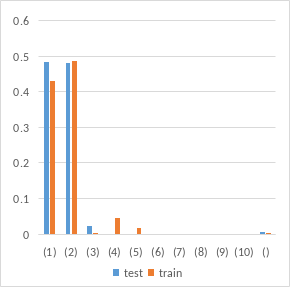
\includegraphics[width=0.31\linewidth]{figures/relative_frequencies_v10.png}
        \label{fig:relative_frequencies_v10}
    }
    \subfigure[$Lang_{13}$]{
        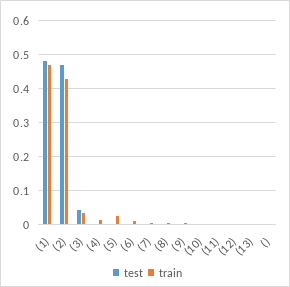
\includegraphics[width=0.31\linewidth]{figures/relative_frequencies_v13.png}
        \label{fig:relative_frequencies_v13}
    }
    \subfigure[$Lang_{100}$, (13 most frequent messages)]{
        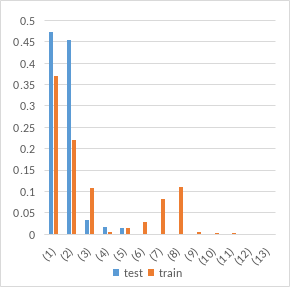
\includegraphics[width=0.31\linewidth]{figures/relative_frequencies_v100.png}
        \label{fig:relative_frequencies_v100}
    }
    \caption{Relative frequencies of messages (ordered by frequency in test dataset)}
    \label{fig:relative_frequencies_vocabularies}
\end{figure}

When looking at the emerged vocabulary \textbf{qualitatively}, a few properties can be seen.
Figure \ref{fig:relative_frequencies_vocabularies} shows an overview of the frequencies of messages in all three emerged languages for the training and the test split.
% SD: I don't understand how test and training set are used in these experiments. In language games one only has a training set and success is measured through the success in the game. It is not possible to have a test set as learning is continuous.
% DK: TODO
Since the tokens themselves are arbitrary, they are ordered by the relative frequency in the messages for the test set and indices for the tokens are added from index 1 for the most frequent token and index $|V|$ for the least frequent token.
By this the languages are easier comparable across different runs and vocabulary sizes.
% SD: I don't understand this.
% DK: TODO
Figure \ref{fig:relative_frequencies_v100} shows only the 13 most frequent message to provide a better overview.
The lesser frequent messages are never used for the test data and each only used one or two times in the train data.

The first property is that when a message is transferred, it consists of only one symbol.
% SD: Is this controlled by the sender. The sender must have some policy how it is assigning messages. Or is it just random? But what makes the sender then to generate a single message vs a longer message. If it is not controlled - how could we implement some policies for message length?
% DK: what do you mean by policy? The sender is only controled by the success of the receiver. If a longer message leads to a better success, it learns to prodcue longer messages. TODO
In some rare cases, also an empty message is communicated.
The models therefore don't learn any compositionality by combining symbols to create new meaning, but rather encode everything in separate symbols.
Secondly, in all three languages, only very few symbols occur with a high frequency, while most of the symbols are used very rarely.
More specifically, two symbols are used in 95\% of the images with $Lang_{10}$ and $Lang_{13}$, while three symbols are used with $Lang_{100}$.
Thirdly, the agents make use of fewer symbols, when presented with unseen test images compared to when communicating about images in the training split.
This is especially visible for $Lang_{100}$.
Symbols that are used for 16,5\% of the training sample are not used at all in test split.
Furthermore, the frequencies in the test split is much more focused on the two most frequent symbols, while it is more distributed around 5 symbols in the train split.
% SD: A table or a graph with these figures?
% DK: is part of the existing figure. The sum of the first two columns (QUESTION)
% SD: Differences between training and testing configuration; what happens during testing, there is no learning involved but the systems see new images but they have to use the same vocabulary?
% DK: exactly

These findings indicate that referring expressions do emerge in each of the newly emerged languages since the agents are able to communicate the correct object.
However, the agents converge towards very few different referring expressions that are made up differently than in English and likely don't rely on the high level attributes \emph{shape}, \emph{color} and \emph{size}.
% SD: Are they? We haven't tested how humans would describe these scene. I see what you mean, but they you have to explain that you count as an English expression a description containing sequences of colour, size and type and then following the Dale and Reiter's algorithm.
% DK: TODO
The similar frequencies across all three languages suggest that a greater vocabulary size $|V|$ doesn't necessarily lead to different referring expressions, but the languages still converge towards two main expressions.
% SD: All this has to do with the sender's policty how to generate messages. We should have varied this policy. I suspect no policy leads just to one message. How is the system motivated to generate more than one symbol?
% DK: TODO

\begin{figure}[ht]
    \centering
    \subfigure[$Lang_{10}$]{
        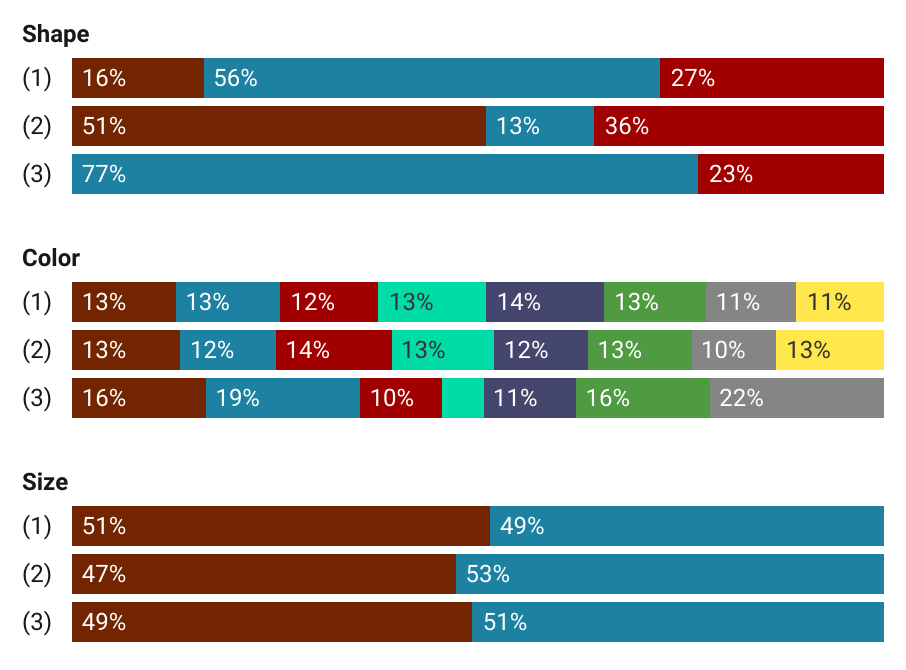
\includegraphics[width=0.31\linewidth]{figures/language_analysis_v10.png}
        \label{fig:language_analysis_v10}
    }
    \subfigure[$Lang_{13}$]{
        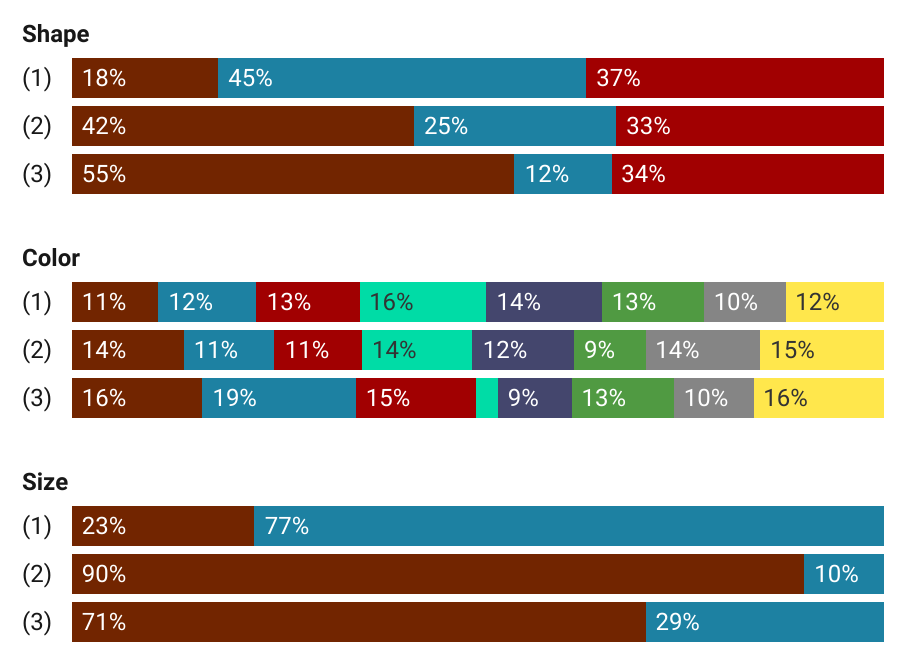
\includegraphics[width=0.31\linewidth]{figures/language_analysis_v13.png}
        \label{fig:language_analysis_v13}
    }
    \subfigure[$Lang_{100}$]{
        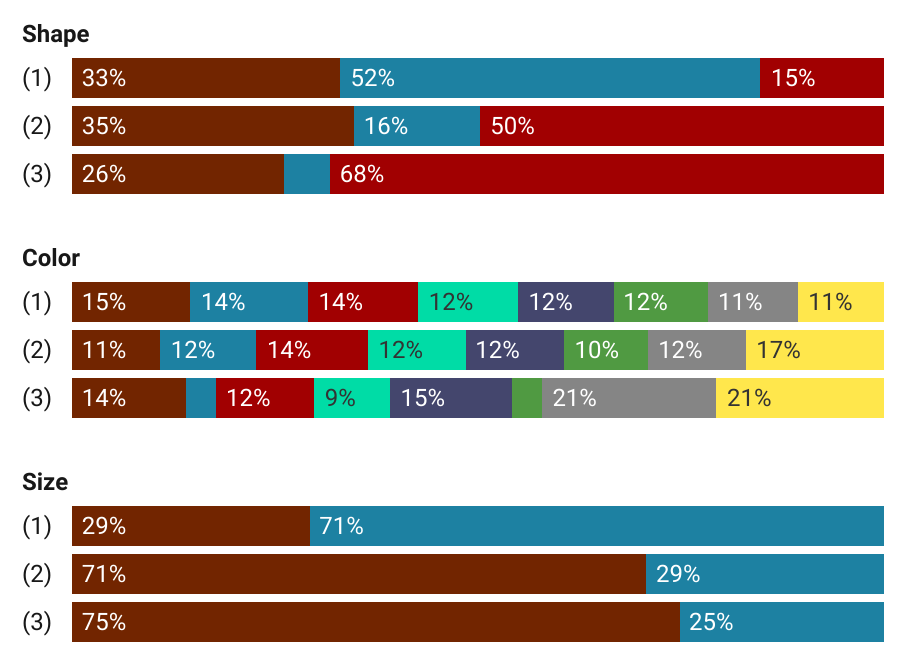
\includegraphics[width=0.31\linewidth]{figures/language_analysis_v100.png}
        \label{fig:language_analysis_v100}
    }
    \caption{Relative share of the described target object's attributes for the top three messages}

    \textbf{Shape:} brown: sphere, blue: cube, red: cylinder \\
    \textbf{Size:} brown: small, blue: large
    \label{fig:language_analysis_vocabularies}
\end{figure}

\cmtDK[inline]{differences in different languages correspond to differences in color prediction of single model caption generation}

Figure \ref{fig:language_analysis_vocabularies} shows the attributes of the target object that are described by each message.
Hereby, the relative share each value of all three attributes are displayed.
For instance the first bar in Figure \ref{fig:language_analysis_v10} shows that 16\% of the target objects that are described with symbol (1) in the language $Lang_{10}$ are spheres.
In the figures, only the three most frequently used messages are included, which make up over 95\% of all messages.

The first thing that can be seen is that different symbols convey different values of attributes.
In the language $Lang_{10}$, symbol (1) is mostly used for target objects that are cubes, while symbol (2) is mostly used for spheres.
There is not much difference for target objects that are cylinders.
The distribution for colors is almost constant across symbols (1) and (2).
Symbol (3) is more frequently used for blue, green and gray objects, while being less used for red, cyan and yellow objects.
This different distribution may also be caused by the much lower absolute usage of symbol (3).
The different sizes are encoded by all symbols in the same way.

Looking at $Lang_{13}$ the symbol usage differs.
The frequencies for the shape look similar, but (the much less used) symbol (3) encodes most of the time spheres instead of cubes.
Again, the colors look similar with small deviations for brown, green and yellow objects.
Most striking however, is the difference for the size.
Symbol (1) is used in 77\% of the cases for large objects, while symbol (2) and (3) are used in 90\% and 71\% of the messages for small objects.

Language $Lang_{100}$ uses symbols its symbols to discriminate cubes and cylinders, while the frequencies for sphere remain constant across all symbols.
The usage for the color is similar to $Lang_{13}$.
Looking at the size, as for $Lang_{13}$, symbol (1) is mostly used to encode small objects, while symbols (2) and (3) are mostly used to encode large objects.

An interesting observation is that symbols are not used for the same attributes across the languages.
In some languages, an attribute is not captured at all by the symbols, while another language heavily relies on it.
The same applies to the values of attributes, especially to the shapes.
Only two of the shapes are distinguished by the usage of symbols, while the third is not captured.
Which shape are encoded, differs from language to language.

Furthermore, these numbers confirm even more that the agents don't rely solely on the human defined attributes.
For instance $Lang_{10}$ only encodes the shape in its symbols.
This would not be enough to distinguish the target object from the distractor consistently.
Following, the agents also encode some additional underlying attributes and patterns to the three above defined attributes.
% SD: But this is slightly problematic, since we strcutured the world this way to emphasise these attributes visually. Hence, a mapping would indicate that the symbols have good semantics if they can discriminate the colours. But this could have to do with the compisitionality issue, perhaps the system was biased to use single word expressions and hence this interfered with the grounding.
% DK: TODO




\newpage

\section{Discussion}
\label{sec:discussion}


\newpage

\section{Conclusion and future work}
\label{sec:conclusion}

\cmtDK[inline]{2 pages}


\addcontentsline{toc}{section}{References}
\bibliography{anthology,personal}

\newpage
\appendix
\section{Resources}
\label{app-resources}



\end{document}


